%%%%%%%%%%%%%%%%%%%%%%%%%%%%%%%%%%%%%%%%%
% Bachelor/Master Thesis 
% LaTeX Template
% Version 2.5 (27/8/17)
%
% This template was downloaded from:
% http://www.LaTeXTemplates.com
%
% Version 2.x major modifications by:
% Vel (vel@latextemplates.com)
%
% This template is based on a template by:
% Steve Gunn (http://users.ecs.soton.ac.uk/srg/softwaretools/document/templates/) 
% Sunil Patel (http://www.sunilpatel.co.uk/thesis-template/)
% 
% Modified by Rostysav Hryniv (2019) and Oleg Farenyuk (2024) 
% 
% Template license:
% CC BY-NC-SA 3.0 (http://creativecommons.org/licenses/by-nc-sa/3.0/)
%
%%%%%%%%%%%%%%%%%%%%%%%%%%%%%%%%%%%%%%%%%

%----------------------------------------------------------------------------------------
%	PACKAGES AND OTHER DOCUMENT CONFIGURATIONS
%----------------------------------------------------------------------------------------

\PassOptionsToPackage{table}{xcolor} % Add table option to xcolor before class loads it

\documentclass[
11pt, % The default document font size, options: 10pt, 11pt, 12pt
oneside, % Two side (alternating margins) for binding by default, uncomment to switch to one side
ukrainian,
english, % ngerman for German
singlespacing, % Single line spacing, alternatives: onehalfspacing or doublespacing
%draft, % Uncomment to enable draft mode (no pictures, no links, overfull hboxes indicated)
%nolistspacing, % If the document is onehalfspacing or doublespacing, uncomment this to set spacing in lists to single
%liststotoc, % Uncomment to add the list of figures/tables/etc to the table of contents
%toctotoc, % Uncomment to add the main table of contents to the table of contents
%parskip, % Uncomment to add space between paragraphs
%nohyperref, % Uncomment to not load the hyperref package
headsepline, % Uncomment to get a line under the header
%chapterinoneline, % Uncomment to place the chapter title next to the number on one line
%consistentlayout, % Uncomment to change the layout of the declaration, abstract and acknowledgements pages to match the default layout
]{BachelorMasterThesis} % The class file specifying the document structure

\usepackage[utf8]{inputenc} % Required for inputting international characters
\usepackage[T1, T2A]{fontenc} % Output font encoding for international characters

\usepackage[ukrainian, english]{babel}

% \usepackage{mathpazo} % Use the Palatino font by default 
  % O.F. Breaks Cyrillic, including Ukrainian, breaks bold, italic, etc. Commented out. The alternative is to use Lualatex.

\usepackage[backend=bibtex,natbib=true]{biblatex} % Use the bibtex backend with the authoryear citation style (which resembles APA)

\addbibresource{bibliography.bib} % The filename of the bibliography

\usepackage[autostyle=true]{csquotes} % Required to generate language-dependent quotes in the bibliography

\usepackage{amsmath}
\usepackage{amssymb}
\usepackage{pifont}
\usepackage{algorithm}
\usepackage{algpseudocode}
\usepackage{booktabs} % For professional tables
\usepackage{subcaption} % For subfigure environment

\newcommand{\cmark}{\ding{51}} % ✓
\newcommand{\xmark}{\ding{55}} % ✗

%----------------------------------------------------------------------------------------
%	MARGIN SETTINGS
%----------------------------------------------------------------------------------------

\geometry{
	paper=a4paper, % Change to letterpaper for US letter
	inner=2.5cm, % Inner margin
	outer=3.8cm, % Outer margin
	bindingoffset=.5cm, % Binding offset
	top=1.5cm, % Top margin
	bottom=1.5cm, % Bottom margin
	%showframe, % Uncomment to show how the type block is set on the page
}

%----------------------------------------------------------------------------------------
%	THESIS INFORMATION
%----------------------------------------------------------------------------------------

\thesistitle{Toward Compact 3D Representations: Geometry-Regularized Gaussian Splatting} % Your thesis title, this is used in the title and abstract, print it elsewhere with \ttitle
\supervisor{Marian \textsc{Petruk}} % Your supervisor's name, this is used in the title page, print it elsewhere with \supname
\examiner{} % Your examiner's name, this is not currently used anywhere in the template, print it elsewhere with \examname
\degree{Bachelor of Science} % Your degree name, this is used in the title page and abstract, print it elsewhere with \degreename
\author{Artem \textsc{Kraievskyi}} % Your name, this is used in the title page and abstract, print it elsewhere with \authorname
\addresses{} % Your address, this is not currently used anywhere in the template, print it elsewhere with \addressname

\subject{Data Science} % Your subject area, this is not currently used anywhere in the template, print it elsewhere with \subjectname
\keywords{} % Keywords for your thesis, this is not currently used anywhere in the template, print it elsewhere with \keywordnames
\university{\href{http://www.ucu.edu.ua}{Ukrainian Catholic University}} % Your university's name and URL, this is used in the title page and abstract, print it elsewhere with \univname
\department{\href{http://apps.ucu.edu.ua}{Faculty of Applied Sciences}} % Your department's name and URL, this is used in the title page and abstract, print it elsewhere with \deptname
\group{\href{http://apps.ucu.edu.ua}{Department of Computer Sciences and Information Technologies}} % Your research group's name and URL, this is used in the title page, print it elsewhere with \groupname
\faculty{\href{http://apps.ucu.edu.ua}{}} % Your faculty's name and URL, this is used in the title page and abstract, print it elsewhere with \facname

\AtBeginDocument{
\hypersetup{pdftitle=\ttitle} % Set the PDF's title to your title
\hypersetup{pdfauthor=\authorname} % Set the PDF's author to your name
\hypersetup{pdfkeywords=\keywordnames} % Set the PDF's keywords to your keywords
}

\begin{document}

\frontmatter % Use roman page numbering style (i, ii, iii, iv...) for the pre-content pages

\pagestyle{plain} % Default to the plain heading style until the thesis style is called for the body content

%----------------------------------------------------------------------------------------
%	TITLE PAGE
%----------------------------------------------------------------------------------------

\begin{titlepage}
\begin{center}

\vspace*{.06\textheight}
{\scshape\LARGE \univname\par}\vspace{1.5cm} % University name
\textsc{\Large Bachelor Thesis}\\[0.5cm] % Thesis type

\HRule \\[0.4cm] % Horizontal line
{\huge \bfseries \ttitle\par}\vspace{0.4cm} % Thesis title
\HRule \\[1.5cm] % Horizontal line
 
\begin{minipage}[t]{0.4\textwidth}
\begin{flushleft} \large
\emph{Author:}\\
\authorname
\end{flushleft}
\end{minipage}
\begin{minipage}[t]{0.4\textwidth}
\begin{flushright} \large
\emph{Supervisor:} \\
\supname
\end{flushright}
\end{minipage}\\[3cm]
 
\vfill

\large \textit{A thesis submitted in fulfillment of the requirements\\ for the degree of \degreename}\\[0.3cm] % University requirement text
\textit{in the}\\[0.4cm]
\groupname\\\deptname\\[2cm] % Research group name and department name
 
\vfill

\includegraphics[height=2.5cm]{UCU_APPS_logo} % University/department logo - uncomment to place it
% Logo taken from the official brandbook: https://ucu.edu.ua/brandbook/brand-book-sources/
% UCU_APPS_logo.pdf 

\vfill
{\large Lviv 2026}\\[4cm] % Date
 
\vfill
\end{center}
\end{titlepage}

%----------------------------------------------------------------------------------------
%	DECLARATION PAGE
%----------------------------------------------------------------------------------------

% \begin{declaration}
% \addchaptertocentry{\authorshipname} % Add the declaration to the table of contents
% \noindent I, \authorname, declare that this thesis titled, \enquote{\ttitle} and the work presented in it are my own. I confirm that:

% \begin{itemize} 
% \item This work was done wholly or mainly while in candidature for a research degree at this University.
% \item Where any part of this thesis has previously been submitted for a degree or any other qualification at this University or any other institution, this has been clearly stated.
% \item Where I have consulted the published work of others, this is always clearly attributed.
% \item Where I have quoted from the work of others, the source is always given. With the exception of such quotations, this thesis is entirely my own work.
% \item I have acknowledged all main sources of help.
% \item Where the thesis is based on work done by myself jointly with others, I have made clear exactly what was done by others and what I have contributed myself.\\
% \end{itemize}
 
% \noindent Signed:\\
% \rule[0.5em]{25em}{0.5pt} % This prints a line for the signature
 
% \noindent Date:\\
% \rule[0.5em]{25em}{0.5pt} % This prints a line to write the date
% \end{declaration}

% \cleardoublepage

%----------------------------------------------------------------------------------------
%	QUOTATION PAGE 
%----------------------------------------------------------------------------------------

\vspace*{0.2\textheight}

\noindent\enquote{\itshape Que sera, sera,\\
Whatever will be, will be;\\
The future's not ours to see.\\
Que sera, sera.}\bigbreak

\hfill Jay Livingston and Ray Evans

%----------------------------------------------------------------------------------------
%	ABSTRACT PAGE
%----------------------------------------------------------------------------------------

\begin{abstract}
\addchaptertocentry{\abstractname}

\noindent Standard 3D Gaussian Splatting (3DGS) achieves real-time novel-view synthesis but optimizes purely for photometric consistency, producing geometrically unreliable surface reconstructions with model sizes exceeding 500~MB per scene — limiting deployment on mobile devices and in AR/VR applications.

We propose a unified geometry-regularized 3DGS framework that integrates five modular geometric priors: depth consistency (DUSt3R), surface normal supervision (DUSt3R), planar co-planarity constraints (SAM~3), edge-aware adaptive densification, and mesh-based TSDF regularization. The central research question is which geometric constraints — individually and in combination — most effectively reduce model size without sacrificing rendering quality.

To answer this, we conduct a systematic ablation study across all $2^5 = 32$ prior combinations on three indoor scenes from the Deep Blending dataset. Individual geometric priors (depth, normals, planarity, mesh) each maintain rendering quality within $\pm$0.04~dB of the 27.88~dB baseline — their impact is primarily in combination: depth paired with planarity achieves 27.92~dB PSNR (+0.04~dB). Edge-aware adaptive densification is the most practically impactful component, reducing the Gaussian primitive count by 32\% (from 1{,}560K to 1{,}060K, 369~MB to 250~MB) with a PSNR drop of only 0.3~dB — a trade-off imperceptible under normal viewing conditions.

These results demonstrate that geometry-regularized 3DGS can be deployed in memory-constrained environments without meaningful loss of visual quality, enabling viable use on mobile devices and in AR/VR systems. The proposed ablation framework further provides the research community with a systematic, evidence-based methodology for selecting geometric constraints, replacing ad hoc design decisions with principled configuration choices.
\end{abstract}


%----------------------------------------------------------------------------------------
%	ACKNOWLEDGEMENTS
%----------------------------------------------------------------------------------------

\begin{acknowledgements}
\addchaptertocentry{\acknowledgementname} % Add the acknowledgements to the table of contents
I would like to express my sincere gratitude to my supervisor, Marian Petruk, for his invaluable guidance, patience, and insightful feedback throughout the duration of this project. His expertise was instrumental in shaping the direction of my research.

I also wish to thank the faculty of the Faculty of Applied Sciences at Ukrainian Catholic University for providing the resources and environment necessary to complete this work.

I am likewise grateful to the entire UCU ML Lab team, whose inspiration and guidance were a constant support throughout my research.

Finally, a special thank you to my family for their unwavering encouragement and support.
\end{acknowledgements}

%----------------------------------------------------------------------------------------
%	LIST OF CONTENTS/FIGURES/TABLES PAGES
%----------------------------------------------------------------------------------------

\tableofcontents % Prints the main table of contents

\listoffigures % Prints the list of figures

\listoftables % Prints the list of tables

%----------------------------------------------------------------------------------------
%	ABBREVIATIONS
%----------------------------------------------------------------------------------------

\begin{abbreviations}{ll}

\textbf{3DGS}   & 3D Gaussian Splatting \\
\textbf{AR/VR}  & Augmented Reality / Virtual Reality \\
\textbf{COLMAP} & Colmap Structure-from-Motion and MVS pipeline \\
\textbf{CUDA}   & Compute Unified Device Architecture \\
\textbf{DUSt3R} & Dense Unconstrained Stereo 3D Reconstruction \\
\textbf{GPU}    & Graphics Processing Unit \\
\textbf{LSD}    & Line Segment Detector \\
\textbf{LPIPS}  & Learned Perceptual Image Patch Similarity \\
\textbf{MSE}    & Mean Squared Error \\
\textbf{MVS}    & Multi-View Stereo \\
\textbf{NeRF}   & Neural Radiance Field \\
\textbf{PLY}    & Polygon File Format \\
\textbf{PSNR}   & Peak Signal-to-Noise Ratio \\
\textbf{RGB}    & Red, Green, Blue \\
\textbf{SAM}    & Segment Anything Model \\
\textbf{SAM~3}  & Segment Anything with Concepts (version 3) \\
\textbf{SfM}    & Structure-from-Motion \\
\textbf{SSIM}   & Structural Similarity Index Measure \\
\textbf{TSDF}   & Truncated Signed Distance Function \\
\textbf{VIO}    & Visual-Inertial Odometry \\
\textbf{VRAM}   & Video Random Access Memory \\

\end{abbreviations}

%----------------------------------------------------------------------------------------
%	SYMBOLS
%----------------------------------------------------------------------------------------

\begin{symbols}{lll}

$\mathcal{G}$           & Set of Gaussian primitives        & --- \\
$K$                     & Total number of Gaussian primitives & --- \\
$N$                     & Number of training images          & --- \\
$\boldsymbol{\mu}_k$    & 3D center of the $k$-th Gaussian  & $\mathbb{R}^3$ \\
$\boldsymbol{\Sigma}_k$ & Covariance matrix of the $k$-th Gaussian & $\mathbb{R}^{3\times3}$ \\
$\alpha_k$              & Opacity of the $k$-th Gaussian    & $[0,1]$ \\
$\mathbf{n}$            & Surface normal vector              & $\mathbb{R}^3$ \\

\addlinespace

$\mathcal{L}$           & Total training loss                & --- \\
$\lambda_d$             & Weight for depth prior loss        & --- \\
$\lambda_n$             & Weight for normal prior loss       & --- \\
$\lambda_p$             & Weight for planar constraint loss  & --- \\
$\lambda_e$             & Weight for edge normal loss        & --- \\
$\lambda_m$             & Weight for mesh regularization loss & --- \\

\addlinespace

$\gamma$                & Gradient-magnitude threshold for Gaussian splitting & --- \\

\addlinespace

$\mathbf{K}$            & Camera intrinsic matrix            & $\mathbb{R}^{3\times3}$ \\
$\mathbf{R}$            & Rotation matrix                    & $\mathbb{R}^{3\times3}$ \\
$\mathbf{t}$            & Translation vector                 & $\mathbb{R}^3$ \\
$\mathbf{u}$            & 2D image pixel coordinate          & $\mathbb{R}^2$ \\
$D$                     & Depth map                          & --- \\

\end{symbols}

%----------------------------------------------------------------------------------------
%	DEDICATION
%----------------------------------------------------------------------------------------

\dedicatory{To my beloved ones} 

%----------------------------------------------------------------------------------------
%	THESIS CONTENT - CHAPTERS
%----------------------------------------------------------------------------------------

\mainmatter % Begin numeric (1,2,3...) page numbering

\pagestyle{thesis} % Return the page headers back to the "thesis" style

% Include the chapters of the thesis as separate files from the Chapters folder
% Uncomment the lines as you write the chapters
% Remember -- some filesystems are case sensitive.

\chapter{Introduction}


\section{Motivation}

Modern computer vision and graphics applications -- from AR/VR systems to robotics and real-time rendering -- depend critically on 3D scene representations that are both compact and geometrically accurate. In AR/VR, for instance, convincing user experiences require precise geometry: objects must stay anchored in place, occlusions need to look correct, and the overall spatial structure must remain stable under user movement. At the same time, these systems operate under strict real-time and memory constraints, so representations cannot be arbitrarily large or slow to process. Current 3D Gaussian Splatting approaches often require 500+ MB per scene, making them impractical for deployment on mobile devices or real-time streaming applications. Similar demands arise in robotics, where reliable 3D understanding directly impacts localization, path planning, and safe interaction with the environment -- errors in geometry can have tangible consequences. Likewise, in graphics pipelines tasked with rendering complex scenes, the representation must scale efficiently without sacrificing visual quality.

Recent neural rendering methods have made impressive strides in synthesizing novel views from sparse image sets. Techniques such as Neural Radiance Fields (NeRFs)~\cite{mildenhall2020nerf} and, more recently, 3D Gaussian Splatting (3DGS)~\cite{kerbl20233dgs}, can produce highly photorealistic images by learning scene representations directly from photographs. 3DGS, in particular, stands out for its real-time rendering performance and memory efficiency, making it attractive for interactive and large-scale applications. However, these methods are primarily optimized for appearance fidelity rather than explicit geometric correctness.

A key challenge is that depth and surface structure emerge implicitly in these models rather than being explicitly enforced. Without strong geometric supervision, reconstructed scenes often suffer from depth inconsistencies across viewpoints, incorrect scale, and poorly defined surfaces, especially in challenging regions such as textureless walls or repetitive patterns. Individual primitives are optimized largely independently, which can result in fragmented or noisy surface reconstructions that appear acceptable in rendered images but degrade when evaluated geometrically. As a result, while neural rendering techniques excel at visual synthesis, the underlying 3D structure is frequently unreliable for applications that require accurate surface reconstruction or metrically consistent representations.

Figure~\ref{fig:normal_comparison_intro} makes the geometric quality problem concrete. Surface normal maps encode per-pixel surface orientation and expose geometric inconsistencies that are invisible in standard RGB renders. The red-boxed region is the same across all methods and reveals a clear progression: standard 3DGS produces incoherent, structureless normals in areas that should be flat walls — a sign that the underlying geometry is noisy and fragmented. Many recent methods attempt to address this through geometry-aware initialization (GeoGaussian), planar constraints (PlanarGS), and other structural regularization strategies, each making measurable progress. Our goal in this thesis is not to outperform state-of-the-art methods in rendering quality, but to demonstrate that comparable geometric fidelity can be achieved at a fraction of the storage cost — 222~MB versus 740~MB for vanilla 3DGS — through principled integration of geometric priors and edge-aware adaptive densification.

\begin{figure}[t]
    \centering
    \setlength{\tabcolsep}{2pt}
    \renewcommand{\arraystretch}{0.5}
    \begin{tabular}{cccc}
        \small View 1 & \small View 3 & \small View 4 & \small View 5 \\[2pt]
        % Ground Truth row
        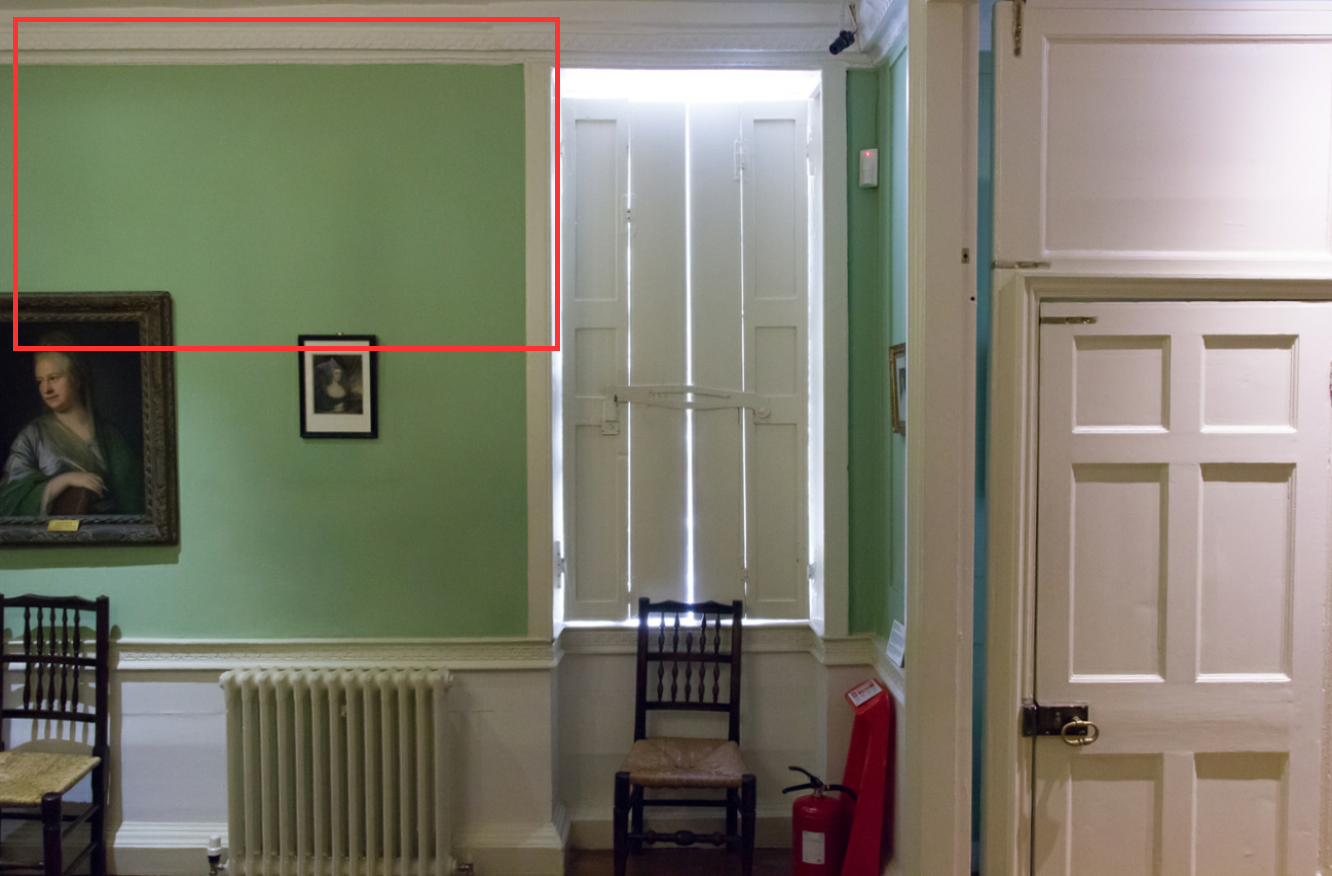
\includegraphics[width=0.235\textwidth]{comparison_figures/drjohnson_gt_view01_rect.png} &
        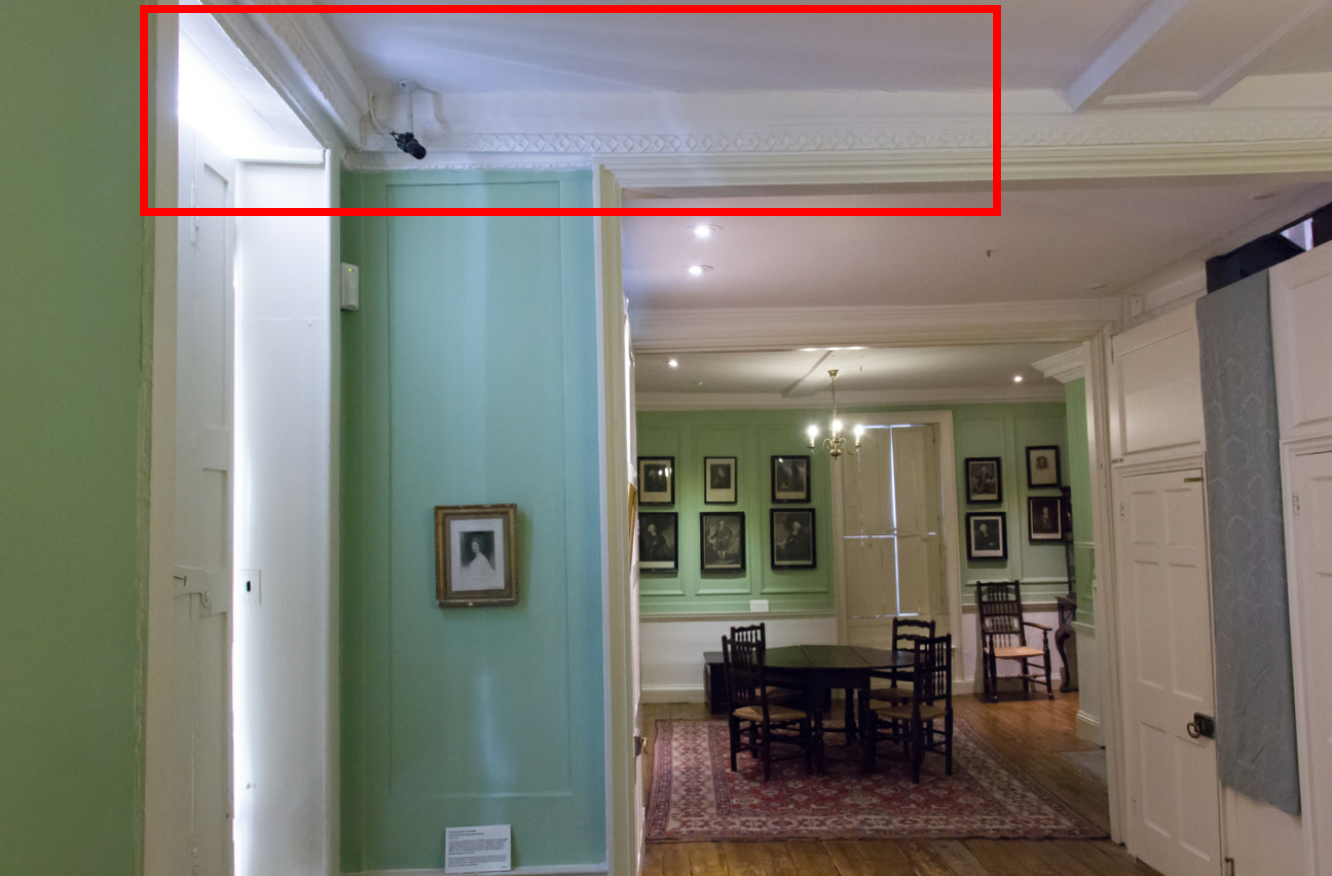
\includegraphics[width=0.235\textwidth]{comparison_figures/drjohnson_gt_view03_rect.png} &
        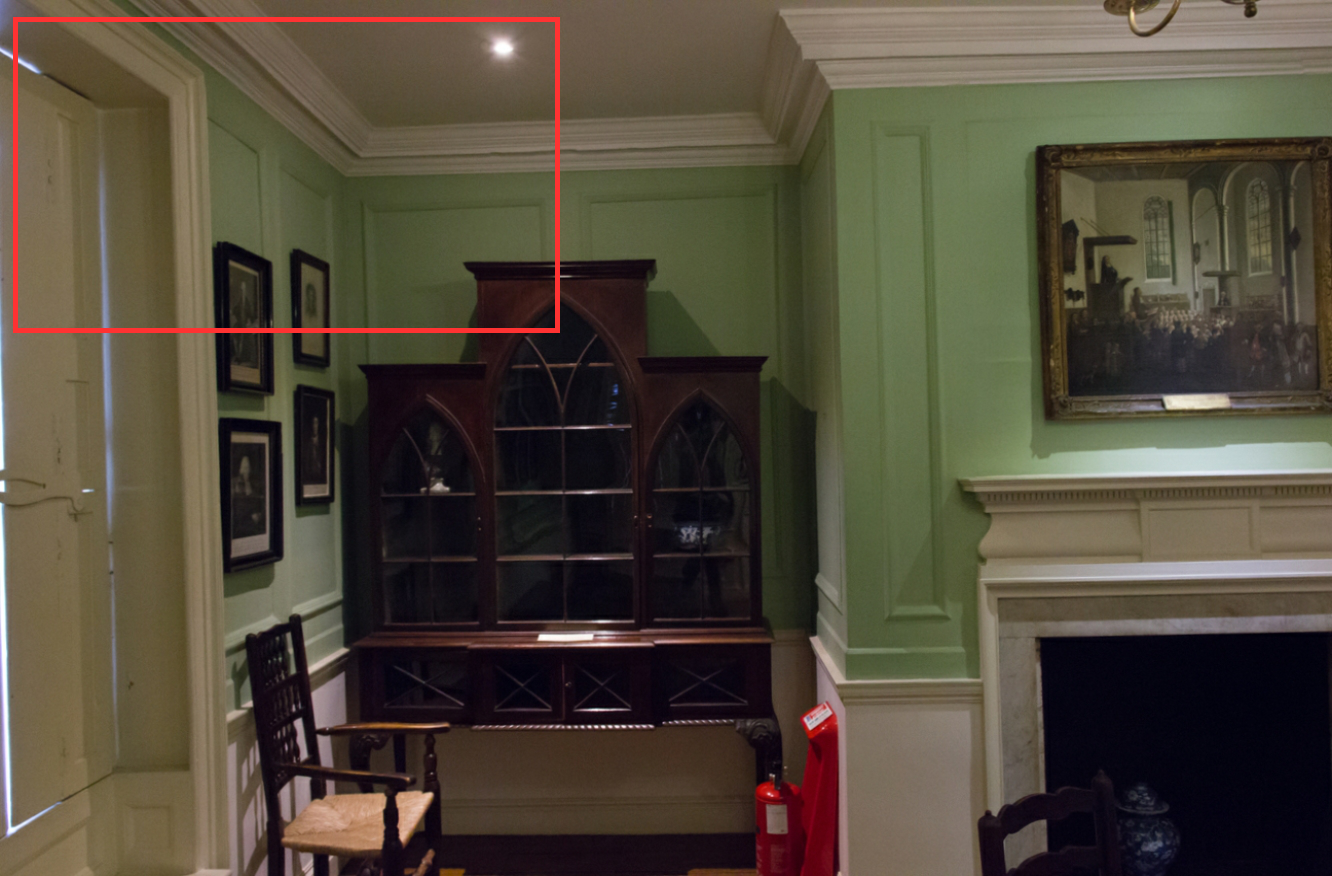
\includegraphics[width=0.235\textwidth]{comparison_figures/drjohnson_gt_view04_rect.png} &
        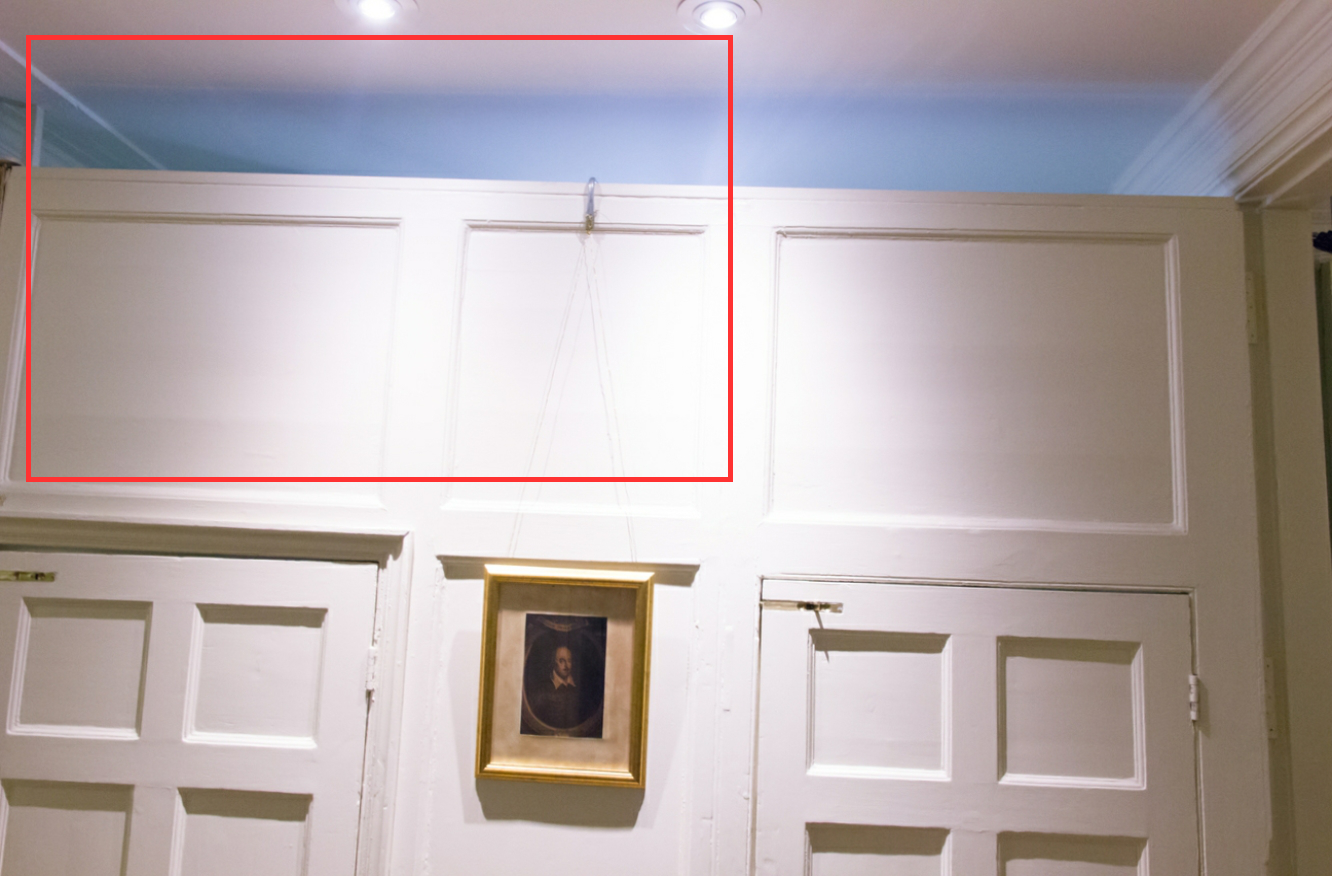
\includegraphics[width=0.235\textwidth]{comparison_figures/drjohnson_gt_view05_rect.png} \\
        \multicolumn{4}{c}{\small\textbf{(a) Ground Truth}} \\[4pt]
        % 3DGS normals
        
\includegraphics[width=0.235\textwidth]{comparison_figures/normal_view01_3DGS_rect.png} &
        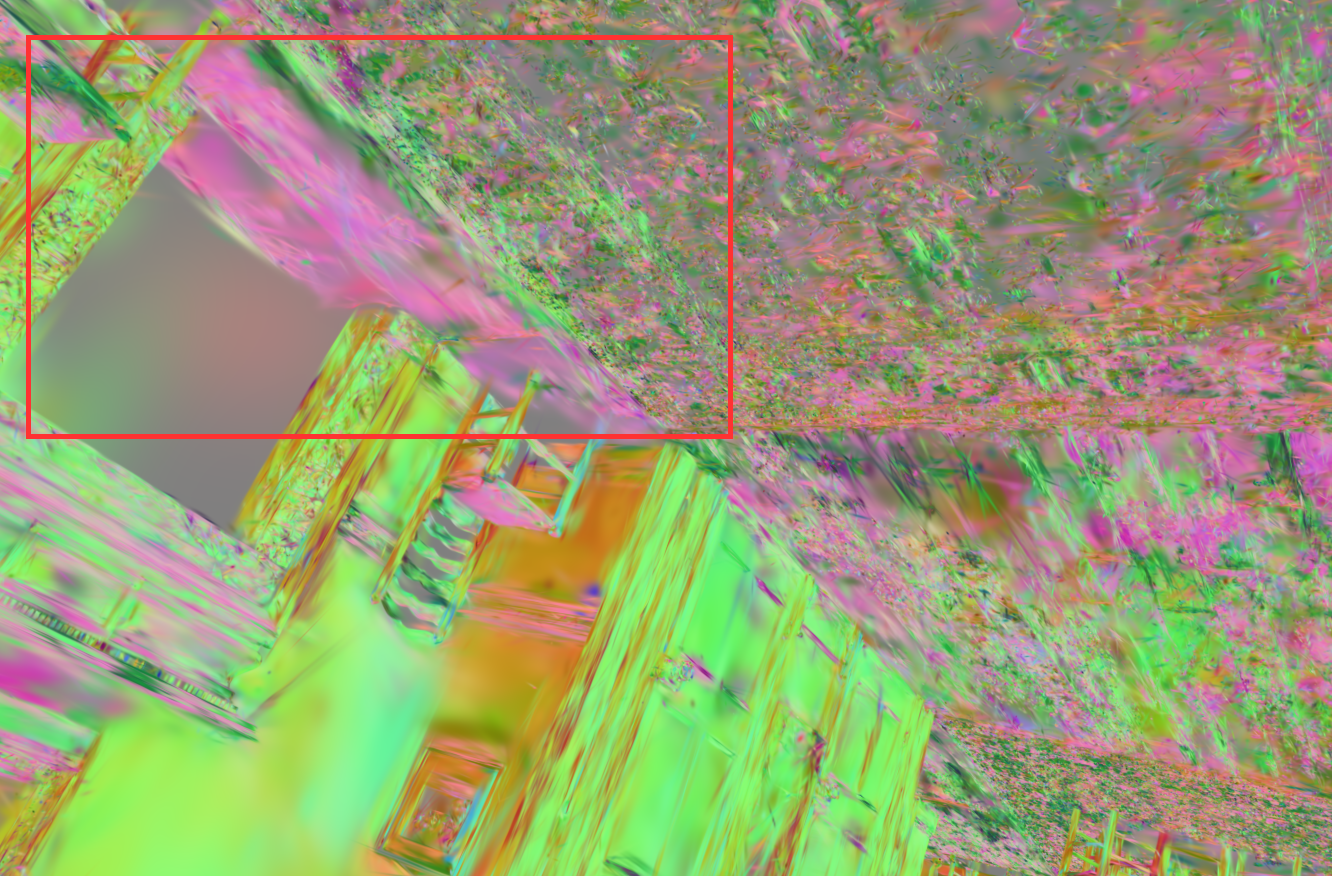
\includegraphics[width=0.235\textwidth]{comparison_figures/normal_view03_3DGS_rect.png} &
        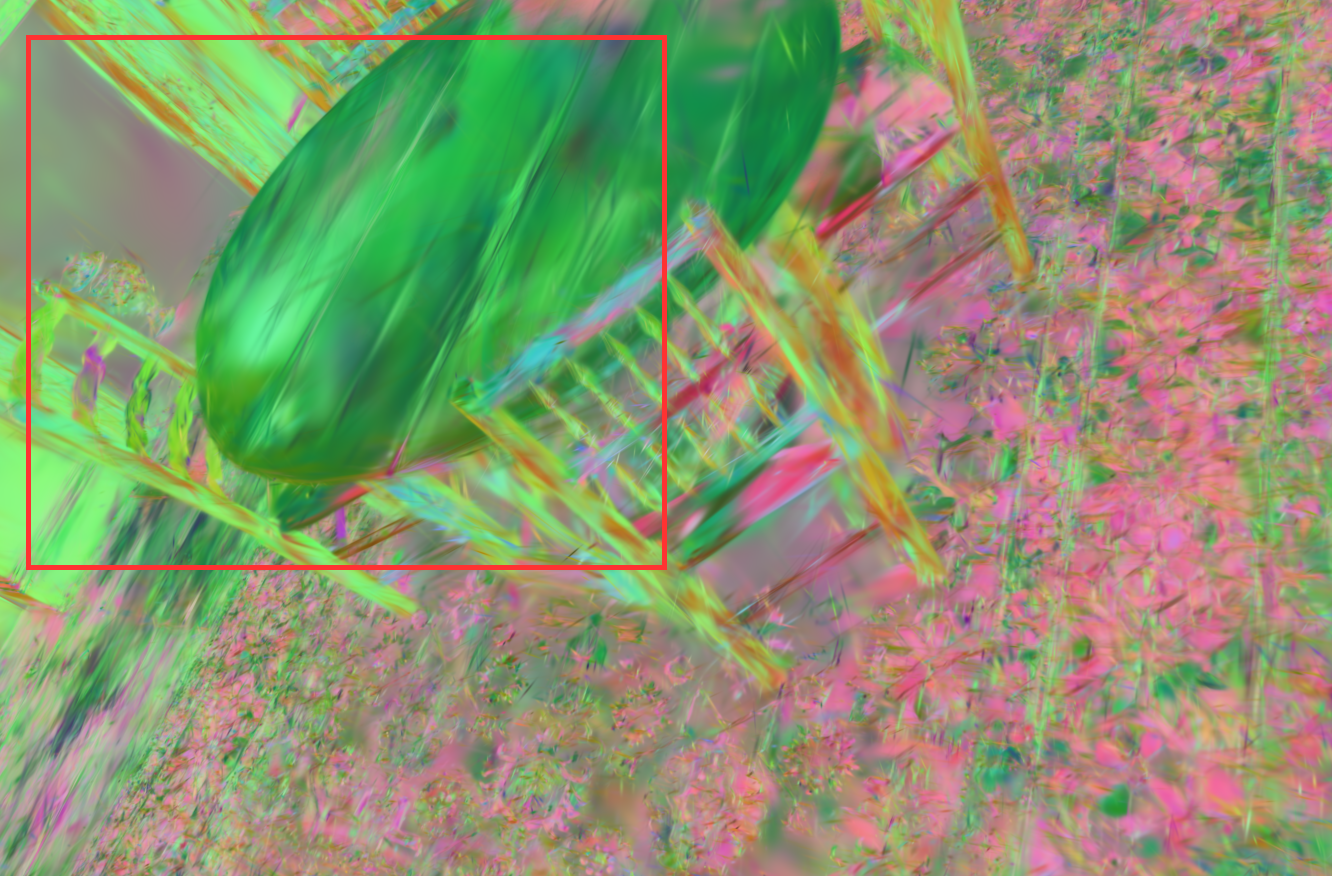
\includegraphics[width=0.235\textwidth]{comparison_figures/normal_view04_3DGS_rect.png} &
        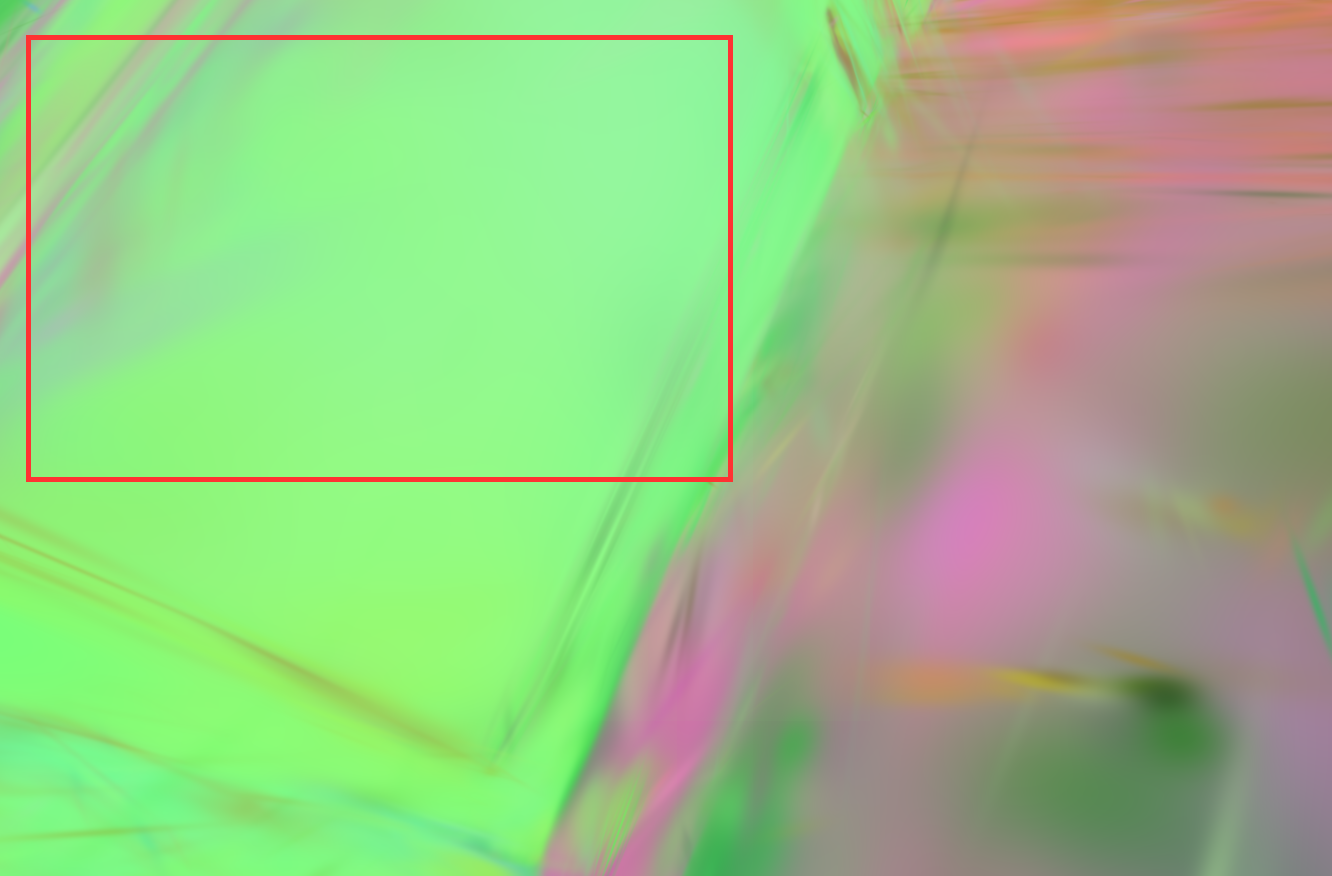
\includegraphics[width=0.235\textwidth]{comparison_figures/normal_view05_3DGS_rect.png} \\
        \multicolumn{4}{c}{\small\textbf{(b) 3D Gaussian Splatting} — 740 MB} \\[4pt]
        % GeoGaussian normals
        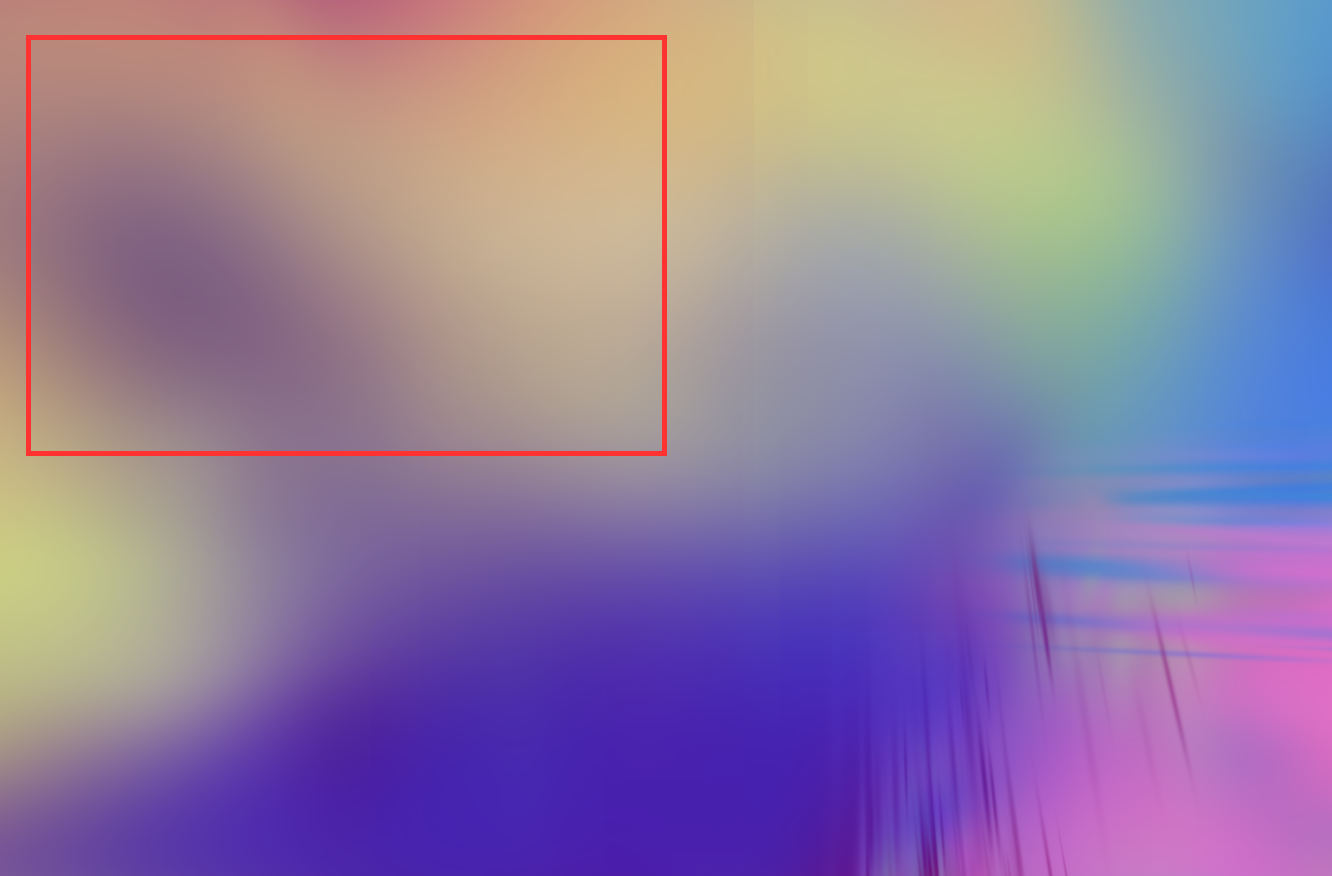
\includegraphics[width=0.235\textwidth]{comparison_figures/normal_view01_GeoGaussian_rect.png} &
        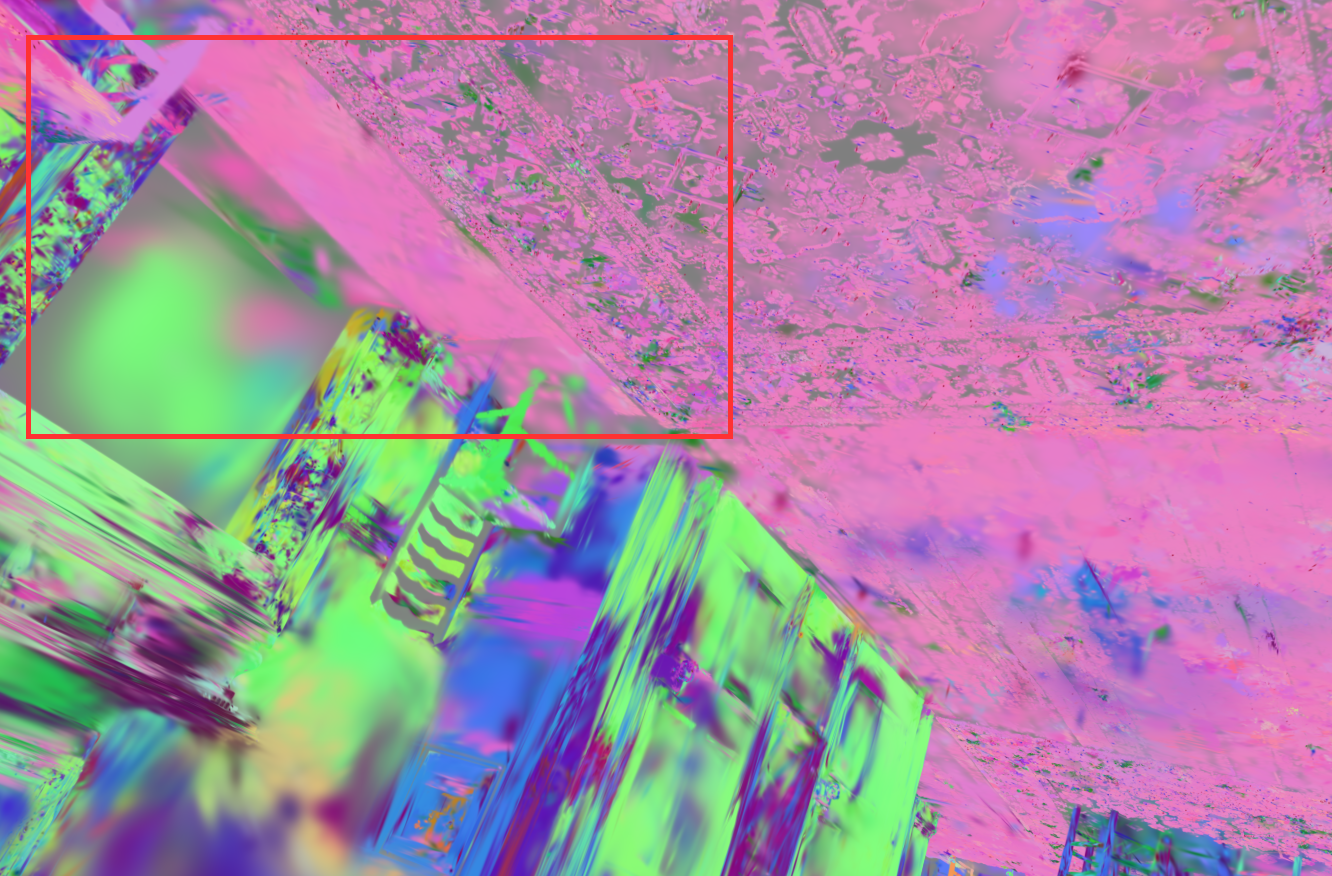
\includegraphics[width=0.235\textwidth]{comparison_figures/normal_view03_GeoGaussian_rect.png} &
        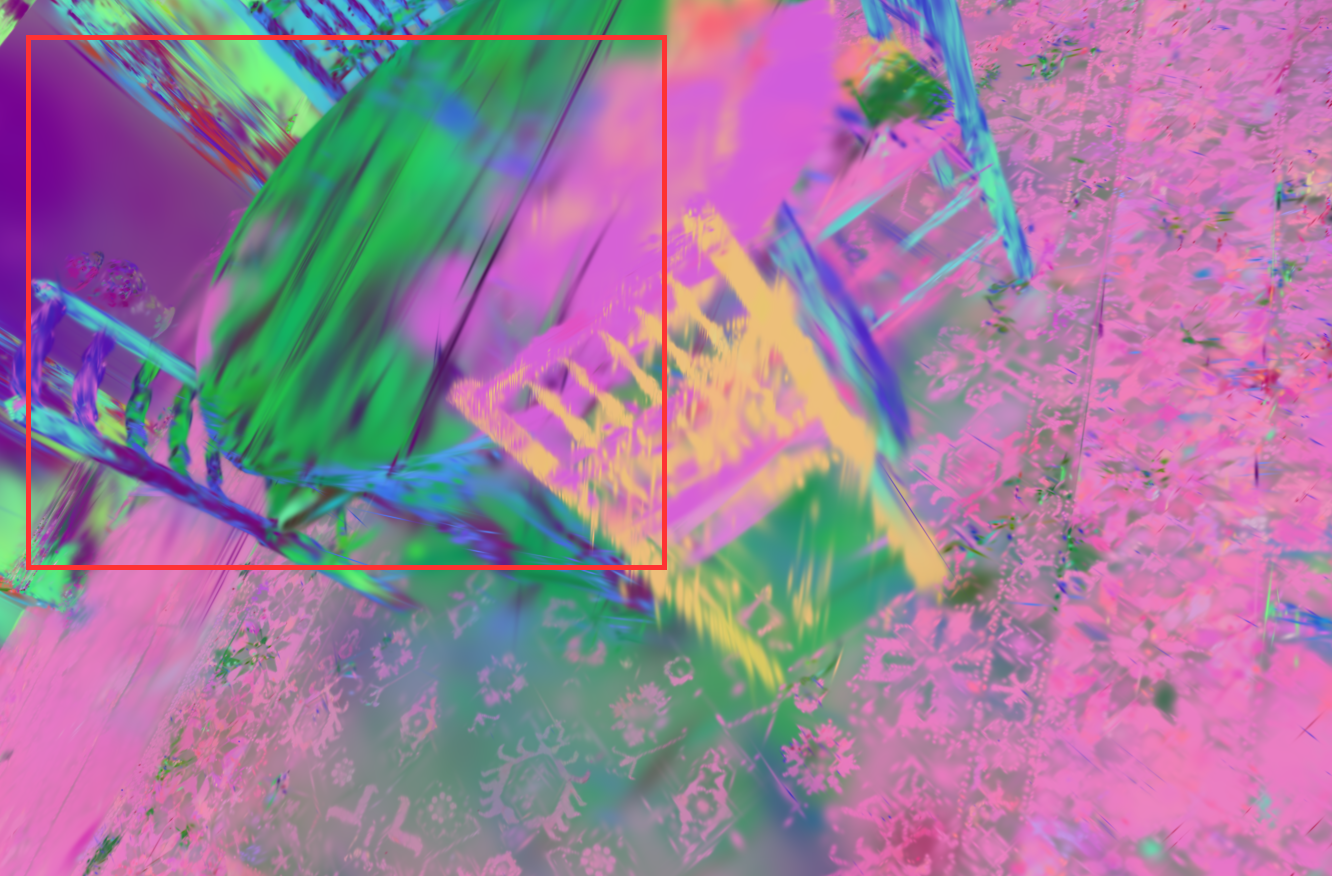
\includegraphics[width=0.235\textwidth]{comparison_figures/normal_view04_GeoGaussian_rect.png} &
        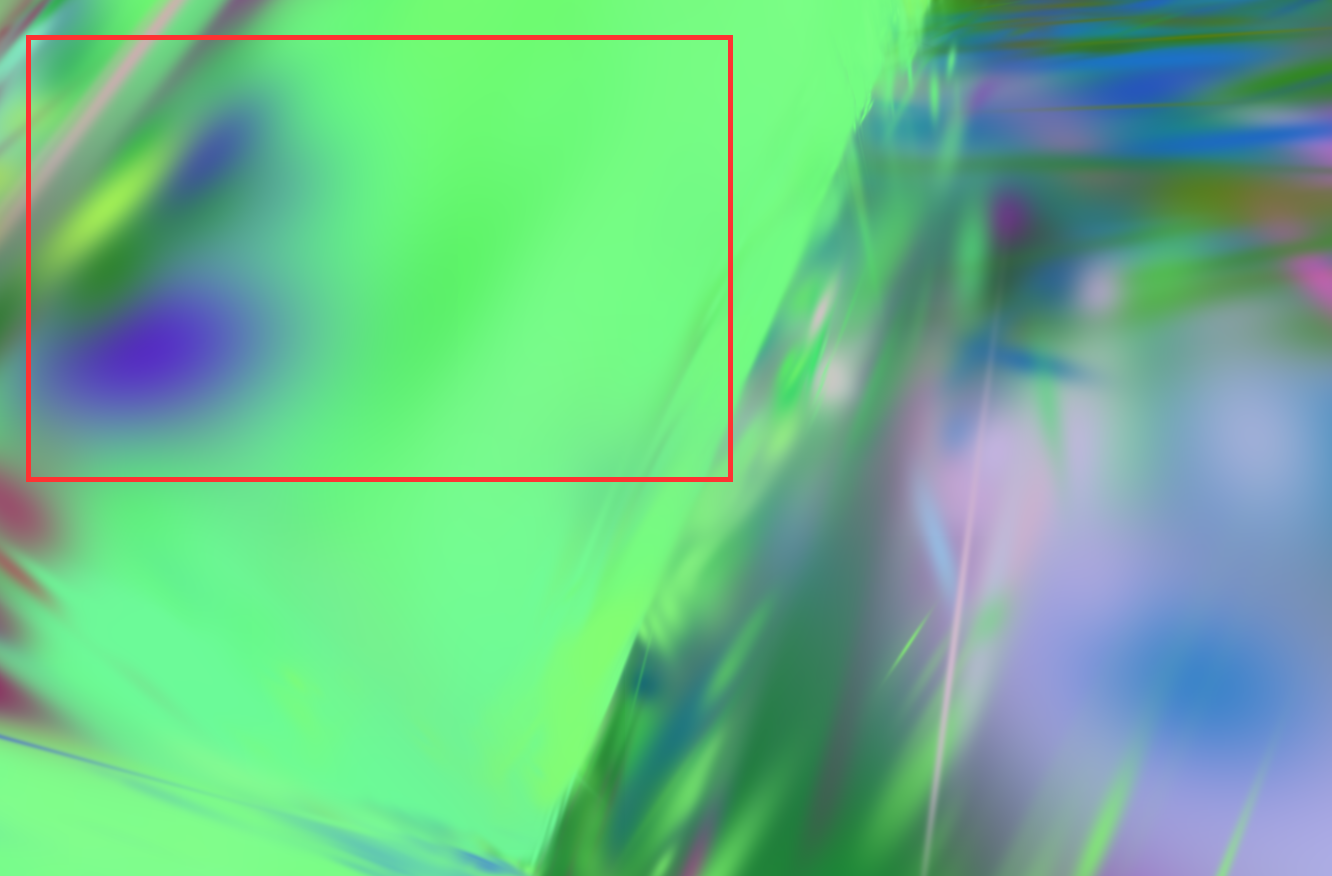
\includegraphics[width=0.235\textwidth]{comparison_figures/normal_view05_GeoGaussian_rect.png} \\
        \multicolumn{4}{c}{\small\textbf{(c) GeoGaussian} — 281 MB} \\[4pt]
        % PlanarGS normals
        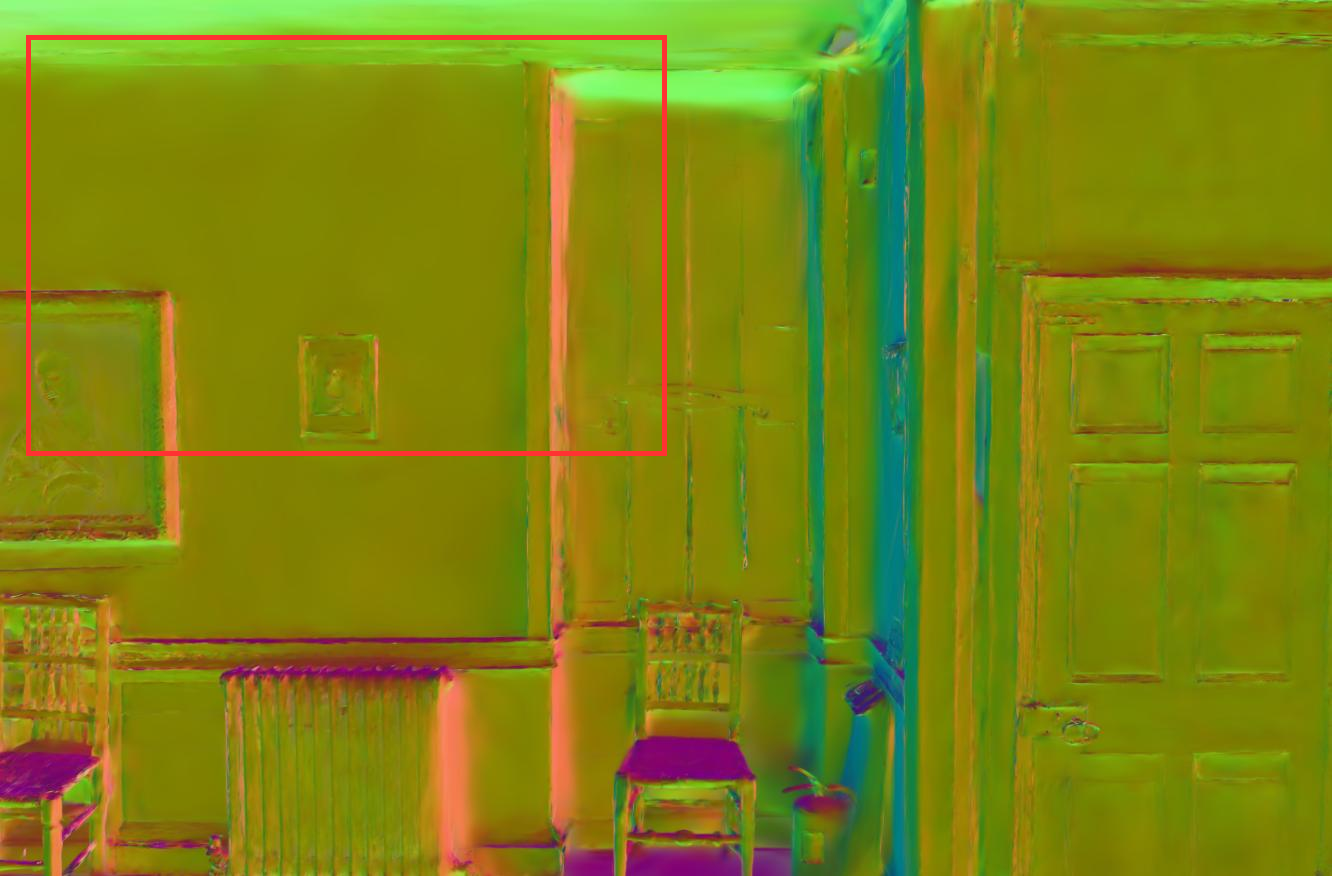
\includegraphics[width=0.235\textwidth]{comparison_figures/normal_view01_PlanarGS_rect.png} &
        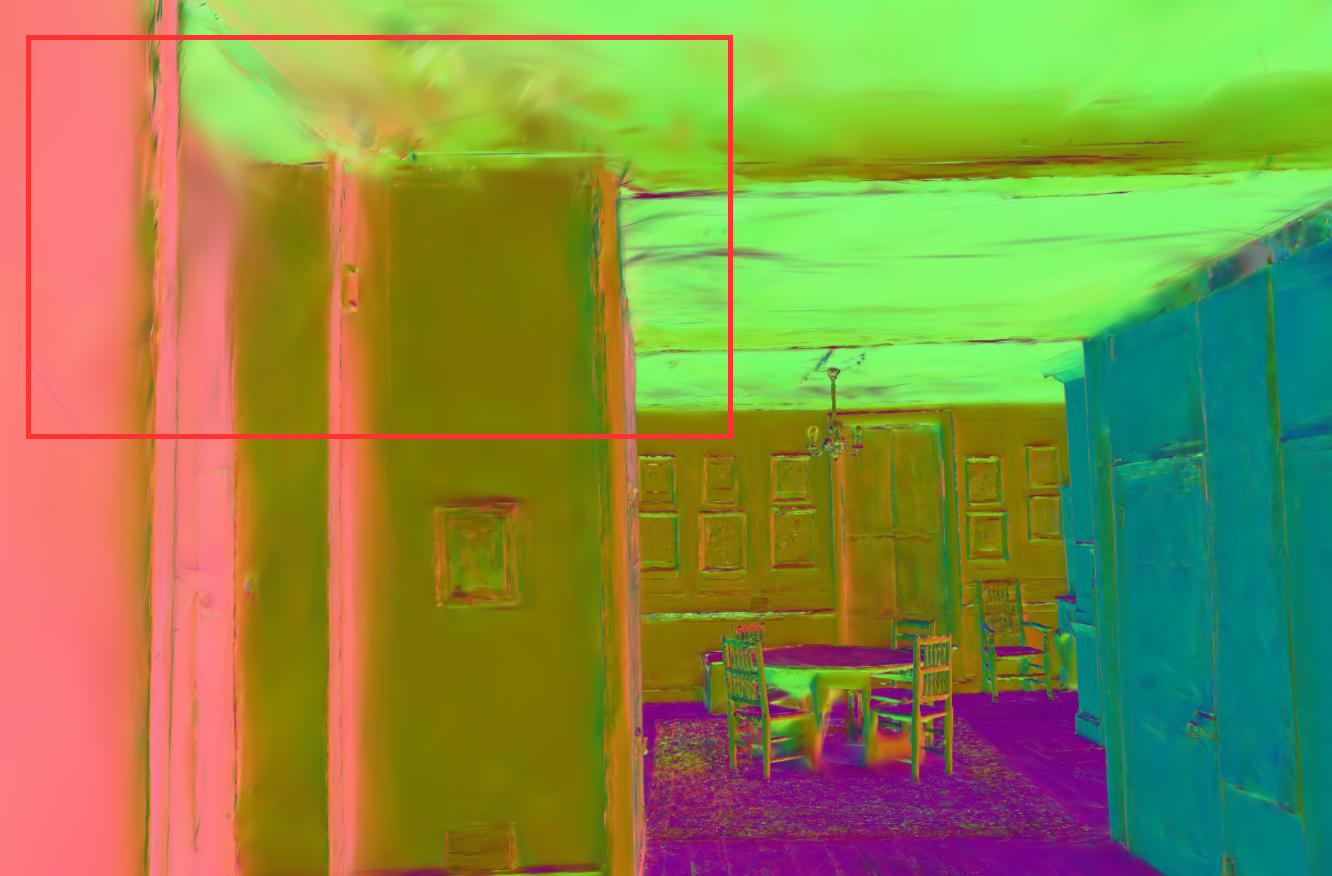
\includegraphics[width=0.235\textwidth]{comparison_figures/normal_view03_PlanarGS_rect.png} &
        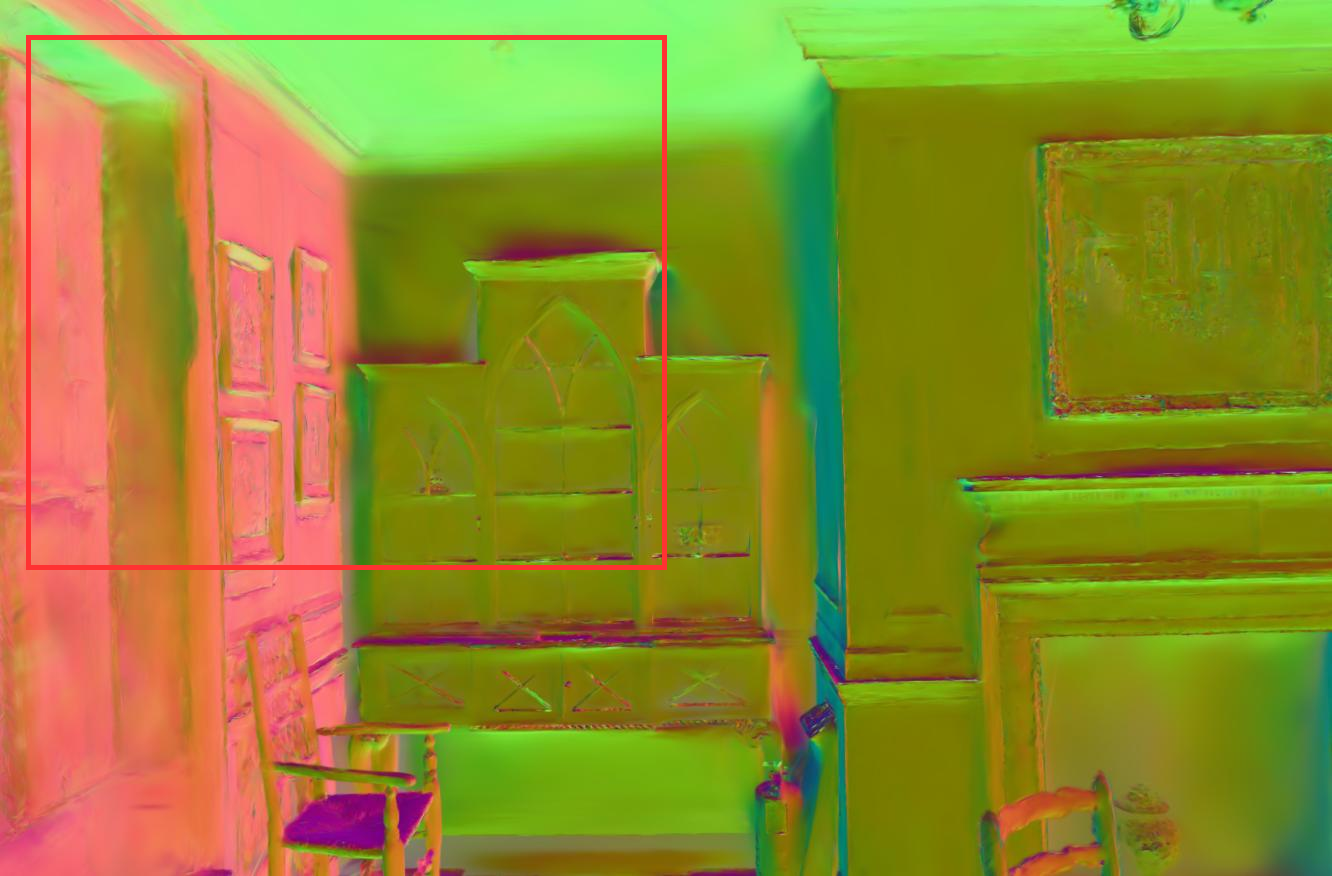
\includegraphics[width=0.235\textwidth]{comparison_figures/normal_view04_PlanarGS_rect.png} &
        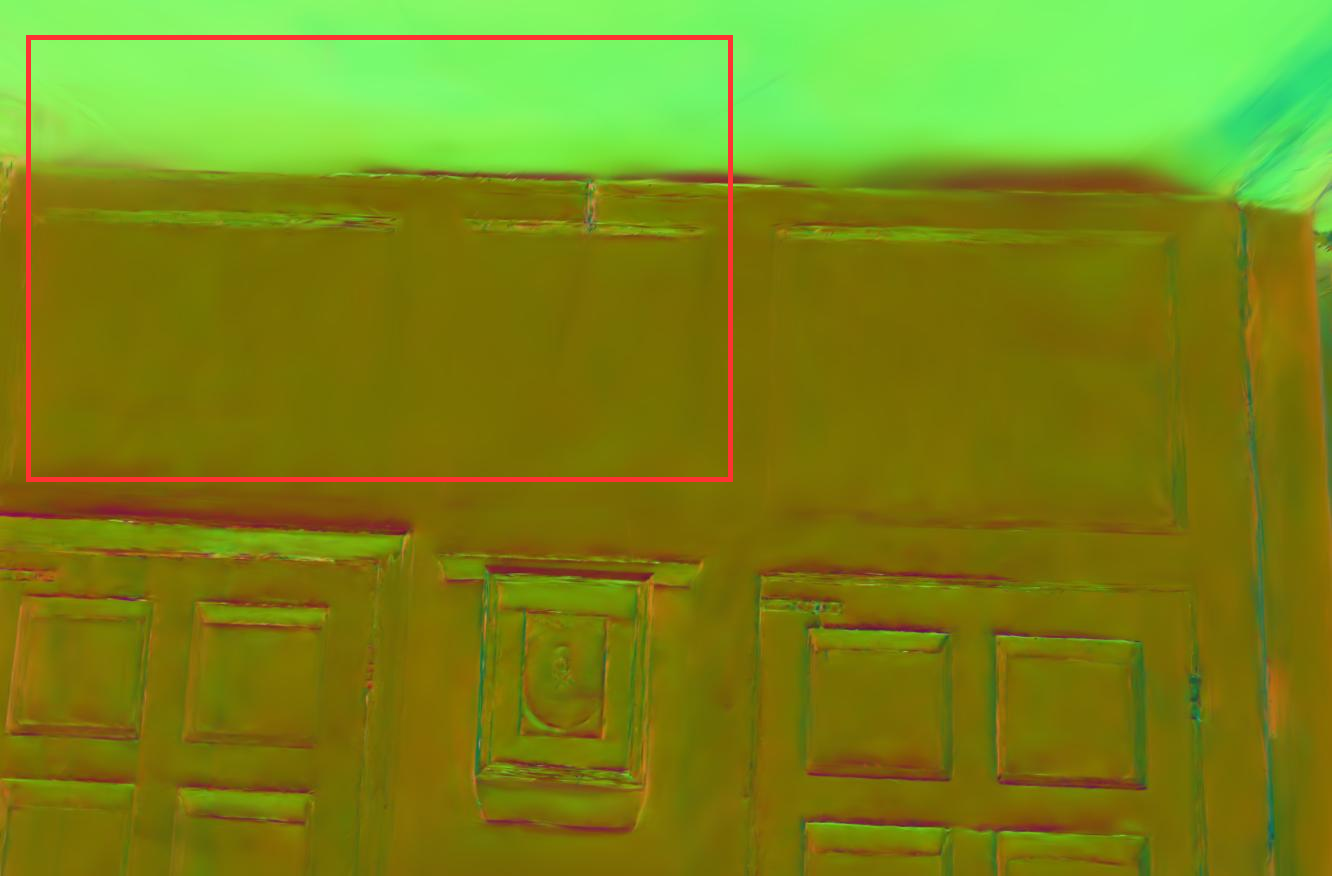
\includegraphics[width=0.235\textwidth]{comparison_figures/normal_view05_PlanarGS_rect.png} \\
        \multicolumn{4}{c}{\small\textbf{(d) PlanarGS} — 410 MB} \\[4pt]
        % Ours normals
        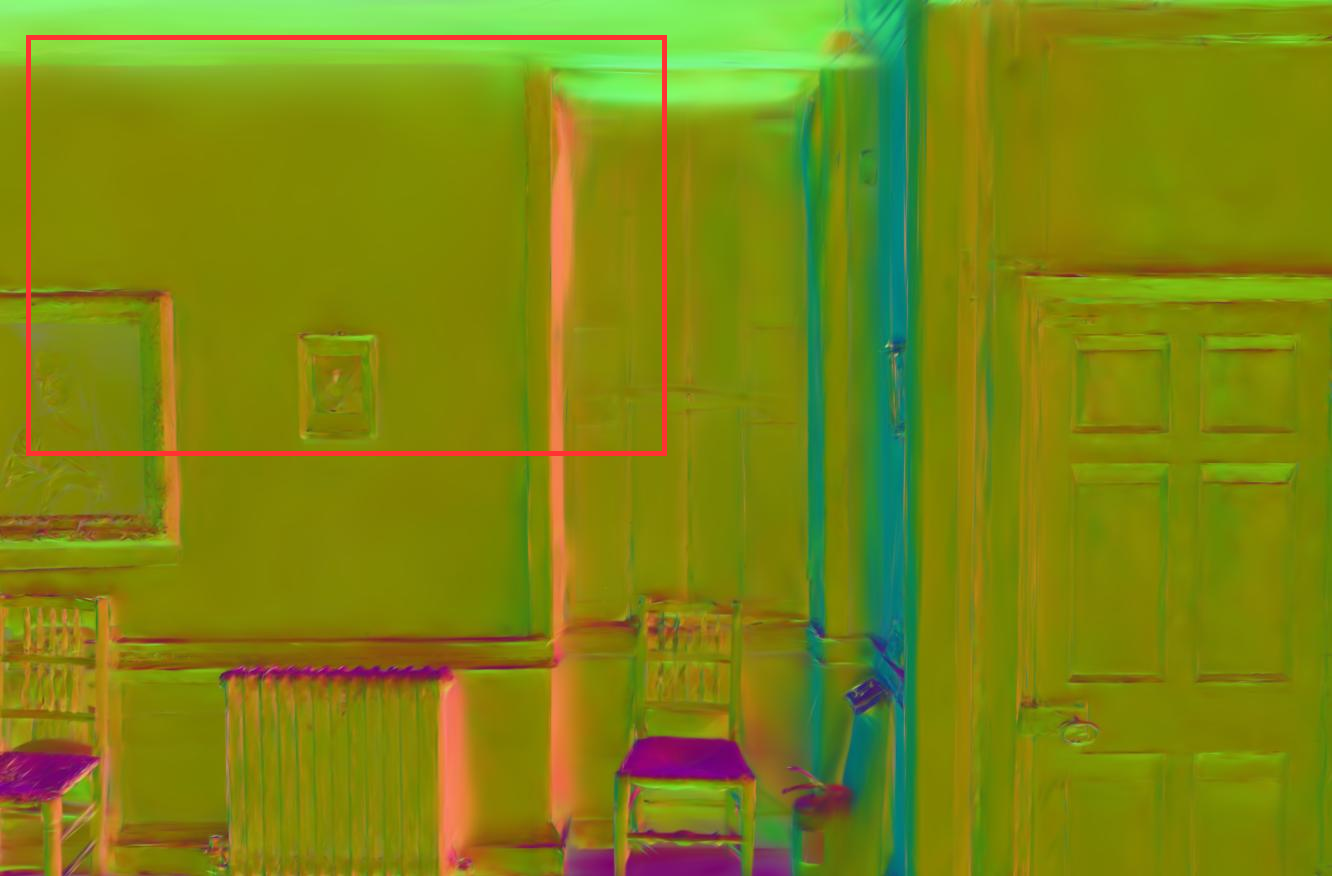
\includegraphics[width=0.235\textwidth]{comparison_figures/normal_view01_Ours_rect.png} &
        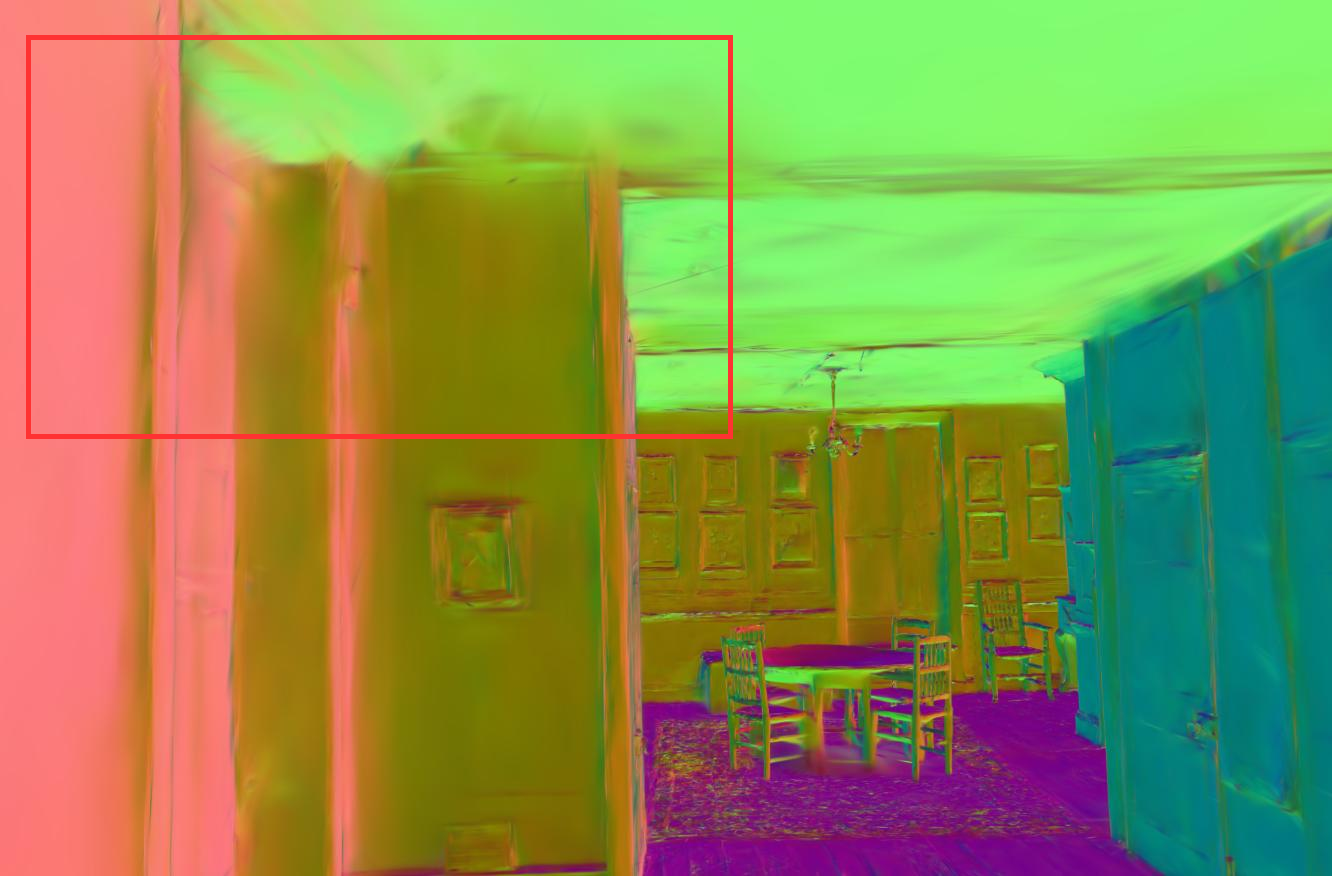
\includegraphics[width=0.235\textwidth]{comparison_figures/normal_view03_Ours_rect.png} &
        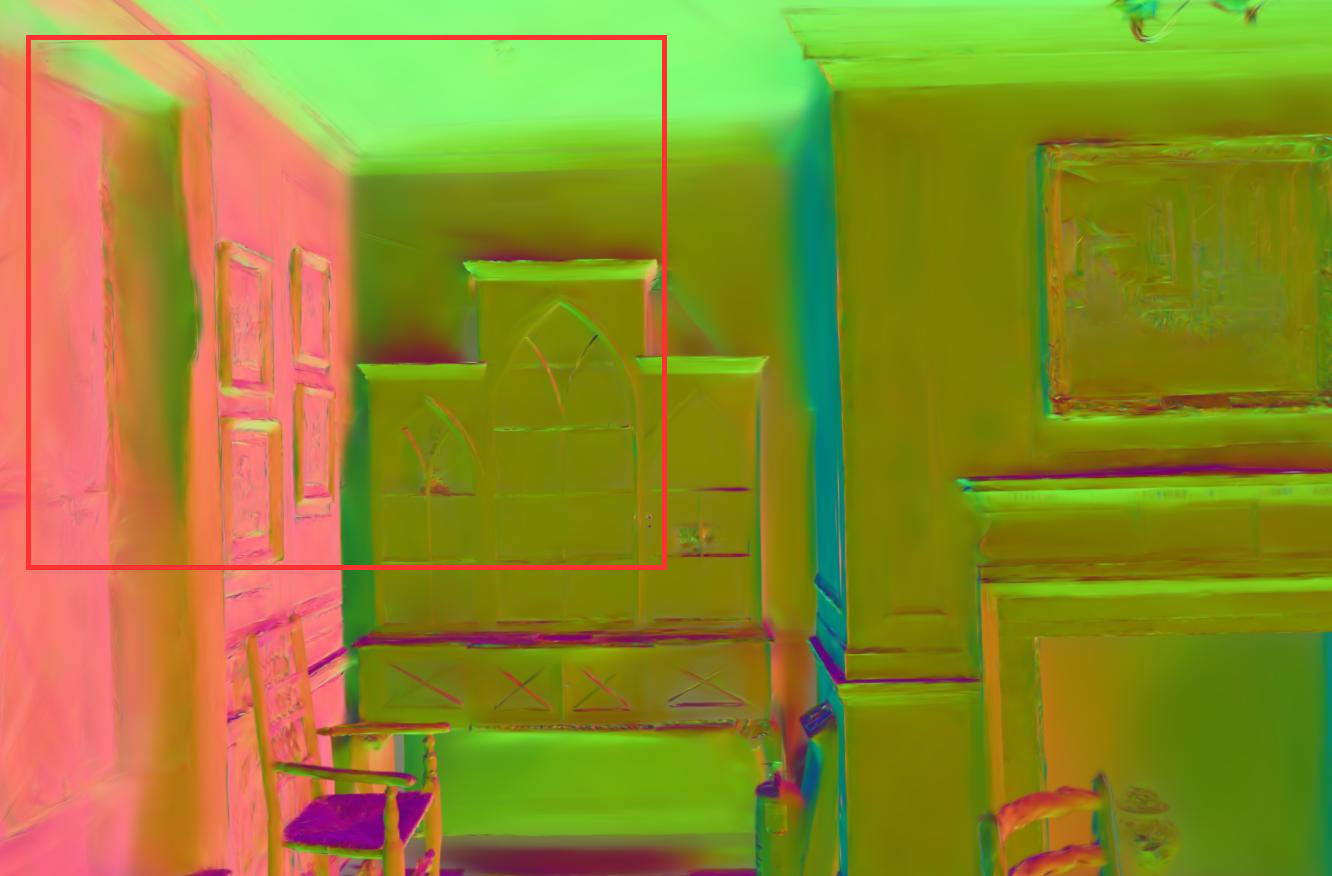
\includegraphics[width=0.235\textwidth]{comparison_figures/normal_view04_Ours_rect.png} &
        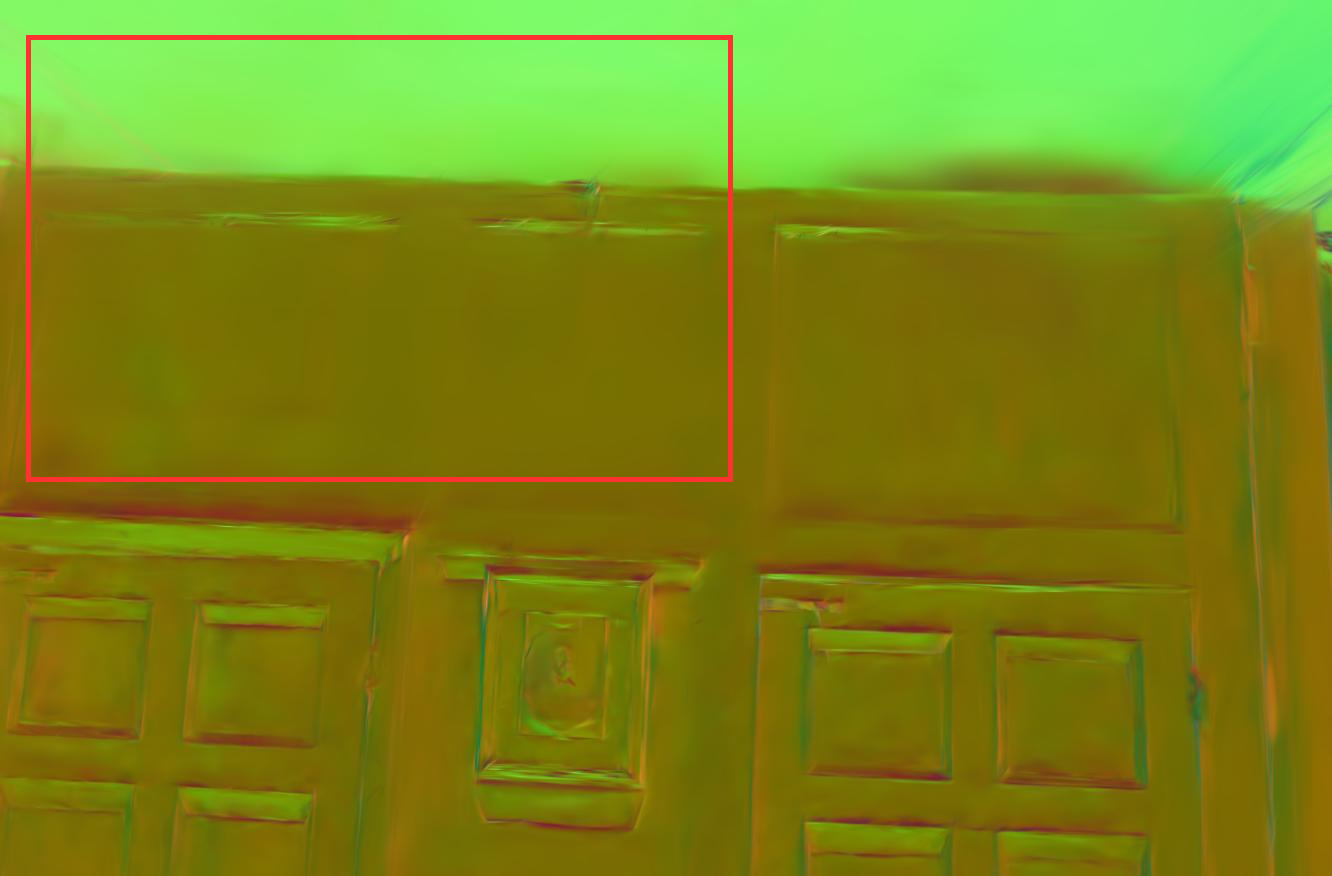
\includegraphics[width=0.235\textwidth]{comparison_figures/normal_view05_Ours_rect.png} \\
        \multicolumn{4}{c}{\small\textbf{(e) Ours (PlanarGS + edge-aware)} — 222 MB} \\
    \end{tabular}
    \caption{Surface normal maps rendered from four DrJohnson viewpoints. Row~(a) shows ground truth RGB images for reference. Rows~(b)--(e) show rendered normals, which directly encode per-pixel surface orientation and reveal geometric quality differences that are invisible in RGB renders. The red rectangle marks the same region across all methods. Standard 3DGS (b) produces incoherent normals with no discernible surface structure in the highlighted region. GeoGaussian (c) shows improvement from geometry-aware initialization but remains noisy. PlanarGS (d) achieves visibly cleaner planar normals. Our method (e) produces the most coherent surfaces, matching PlanarGS quality while storing the scene in only 222~MB — 70\% less than 3DGS.}
    \label{fig:normal_comparison_intro}
\end{figure}

The central question this thesis addresses is: \textit{which geometric priors, individually and in combination, provide the most effective path toward compact yet geometrically faithful 3D Gaussian Splatting representations for structured indoor scenes?}

\section{Contributions}

The contributions of this thesis are summarized as follows:

\begin{itemize}
    \item \textbf{Unified geometry-aware framework:} We propose a unified geometry-aware 3D Gaussian Splatting framework that integrates five complementary geometric modalities: normal priors, depth priors, planar co-planarity constraints, mesh-based regularization through TSDF fusion, and edge-aware adaptive densification. The framework is fully modular, allowing each component to be independently enabled or disabled through command-line flags, facilitating systematic ablation analysis. This design builds upon and extends ideas from GeoGaussian~\cite{geogaussian}, DN-Splatter~\cite{dn_splatter}, PlanarGS~\cite{planargs}, SuGaR~\cite{sugar}, and MILO~\cite{milo2024}, unifying them into a single cohesive pipeline.

    \item \textbf{Comprehensive ablation study across 32 configurations:} We conduct the first comprehensive ablation study that systematically evaluates all $2^5 = 32$ possible combinations of geometric priors (normals, depth, planarity, mesh constraints, and edge-aware control). This systematic exploration quantifies the individual and combined impact of each modality on reconstruction quality, representation compactness, and training efficiency. The study reveals important insights about redundancy, complementarity, and optimal combinations of geometric regularization strategies.

    \item \textbf{Edge-aware adaptive densification:} We introduce a novel edge-aware adaptive densification mechanism that concentrates smaller Gaussians near structural boundaries while using larger, more efficient primitives in planar interiors. This spatially varying strategy improves both geometric fidelity at edges and representation compactness in homogeneous regions, reducing the total primitive count by 30--32\% while maintaining or improving visual quality.

    \item \textbf{Experimental evaluation and practical insights:} We present extensive experimental evaluation on three indoor scenes from the Deep Blending dataset (DrJohnson, Library, and Playroom), using standard metrics (PSNR, SSIM, LPIPS) alongside efficiency measures (Gaussian count, model size, training time). The results provide practical guidance for practitioners on which geometric priors to prioritize based on scene characteristics and application requirements, demonstrating that selective combinations often outperform the full configuration with all priors enabled.
\end{itemize}


\section{Structure Of The Thesis}

This thesis is organized as follows. Chapter~2 reviews related work on recent advances in 3D Gaussian Splatting, with a particular focus on geometry-aware extensions that incorporate depth, normal, surface-based constraints, and planar regularization. Chapter~3 introduces the theoretical background necessary for understanding the proposed approach, including camera geometry, Structure-from-Motion, and 3D Gaussian Splatting fundamentals. Chapter~4 presents the proposed unified framework, detailing the integration of five geometric modalities: normal priors, depth priors, planar constraints, mesh regularization, and edge-aware adaptive densification. Chapter~5 describes the comprehensive experimental methodology and results, including the systematic ablation study across 32 configurations, efficiency analysis, and modality-wise impact assessment on three indoor scenes from the Deep Blending dataset. Finally, Chapter~6 summarizes the main findings, discusses the limitations of the proposed approach, and outlines directions for future work.
\chapter{Related Work}

\section{3D Gaussian Splatting Foundations} 
3D Gaussian Splatting (3DGS) shifts the rendering paradigm from the volumetric ray-marching common in NeRFs to a rasterization-based approach. The scene is represented by a collection of 3D Gaussians, where each primitive is defined by its position, covariance, opacity, and spherical harmonic coefficients. By projecting these primitives onto the image plane and sorting them for alpha-blending, 3DGS achieves real-time rendering speeds while preserving high-frequency details~\cite{kerbl20233dgs}. Standard 3DGS initializes these primitives using sparse point clouds derived from Structure-from-Motion (SfM). During optimization, the method employs an adaptive density control strategy: gradients are monitored to split Gaussians in under-reconstructed areas and prune those with low opacity. However, because the optimization is driven primarily by photometric loss, the resulting geometry often suffers from artifacts. Without explicit geometric regularization, the underlying surface representation tends to be noisy or fragmented, even if the rendered novel views appear visually pleasing.

\section{Initialization Strategies} 
The fidelity of the final reconstruction is heavily dependent on the quality of the initial point cloud. Standard 3DGS creates a strict dependency on sparse SfM data (typically from COLMAP)~\cite{schoenberger2016sfm}, which can act as a bottleneck for challenging captures or large-scale scenes. To mitigate this, methods like GeoGaussian move away from sparse seeds, instead utilizing dense depth and normal priors to align Gaussian orientations with the physical surface from the onset~\cite{li2024geogaussian}. This geometry-aware initialization improves convergence and surface consistency compared to photometry alone.

Recent work by Roman Mutel offers a distinct alternative by bypassing the SfM pipeline entirely. This approach processes RGBD streams from consumer devices (such as the iPhone Pro) and utilizes Visual-Inertial Odometry (VIO) for pose estimation, effectively unprojecting depth maps directly into 3D space. By doing so, the method achieves a linear time complexity \(O(n)\), a significant improvement over the typical polynomial complexity associated with global bundle adjustment, and demonstrates that VIO poses can be sufficiently accurate for training even when traditional feature matching fails.

\section{Depth and Normal Regularization} 
Initialization alone cannot prevent geometric drift during the optimization process. In regions with weak texture or repetitive patterns, photometric loss is an insufficient constraint, leading to “floating” artifacts. DN-Splatter addresses this ill-posed problem by integrating strictly enforced geometric priors. Rather than relying on mesh extraction, it utilizes monocular depth and normal estimates to supervise the training. The key contribution of such methods is the adaptability of the regularization: stronger constraints are applied in areas of high geometric uncertainty, while photometric evidence takes precedence where image data is clear~\cite{dn_splatter}. This balance significantly reduces surface noise, though it primarily focuses on local consistency rather than enforcing a global topology.

\section{Surface-Based Constraints and Structural Representations}
To ensure global geometric coherence, recent methods have attempted to bind Gaussians to explicit surface representations. SuGaR (Surface-Aligned Gaussian Splatting) constrains the primitives to align with a mesh extracted from the density field. By enforcing this alignment, the method acts as a bridge between volumetric rendering and traditional mesh-based graphics, facilitating physics simulations and cleaner surface exports~\cite{sugar}. MiLO extends this idea by placing the mesh “in the loop,” allowing the mesh topology to actively guide the splitting and pruning of Gaussians dynamically~\cite{milo2024}.
A closely related direction explicitly targets planar and structured surfaces, which are especially prominent in indoor scenes. PlanarGS~\cite{planargs} introduces planar primitive modeling into the 3DGS framework by detecting dominant planar surfaces and jointly optimizing both planar parameters and Gaussian primitives. This planar prior enforces stronger global constraints on large flat surfaces such as walls, floors, and ceilings, improving flatness and normal consistency while reducing redundant Gaussians in large planar regions. However, this approach depends on robust plane detection and is primarily tailored to structured indoor geometry.
Another closely related line of work focuses explicitly on surface reconstruction quality from Gaussian representations. PGSR (Point-Guided Gaussian Surface Reconstruction) proposes a Gaussian-based pipeline tailored for high-fidelity surface extraction rather than purely novel view synthesis. The method reconstructs surfaces by deriving depth maps from Gaussian splatting via opacity-weighted integration and subsequently fusing them into a volumetric representation using TSDF. By explicitly optimizing for surface accuracy and leveraging point-guided constraints, PGSR achieves improved surface completeness and normal consistency compared to standard 3DGS pipelines. However, similar to other surface-oriented approaches, PGSR relies on post-hoc depth integration and volumetric fusion, rather than enforcing surface-level constraints directly during Gaussian optimization, which can limit its ability to maintain global structural consistency in large planar indoor scenes~\cite{pgsr}.
IndoorGS further explores structure-aware Gaussian splatting specifically for indoor environments by introducing layout-aware priors and indoor-specific geometric regularization. The method exploits common indoor assumptions such as dominant orthogonal planes and consistent room layouts to stabilize geometry and reduce surface fragmentation. By incorporating scene-level structural cues, IndoorGS demonstrates improved reconstruction consistency in large indoor spaces compared to generic 3DGS pipelines~\cite{indoorgs}.
Another important recent work is GausSurf, which integrates multi-view geometry guidance into the Gaussian splatting optimization process to enhance surface reconstruction quality. GausSurf distinguishes between texture-rich and texture-less regions, leveraging PatchMatch-based multi-view stereo (MVS) geometry for the former and normal priors for the latter. This geometry-guided strategy improves both surface detail and optimization stability, leading to higher-quality surface reconstruction and more efficient training compared to purely photometric or single-modality geometric approaches~\cite{gcaussurf}.
Alternatively, SAGS (Structure-Aware Gaussian Splatting) avoids explicit meshing in favor of implicit structural encoding. It employs a graph-based representation to learn relationships between neighboring primitives, enforcing meaningful spatial coherence without the overhead of managing an explicit mesh. These approaches highlight a trade-off in current literature: mesh-based methods offer tighter geometric coherence and explicit surface extraction, while implicit structural representations provide more compact geometry with reduced memory footprints.

\section{Research Gap} 
Current literature largely treats geometric priors in isolation. Methods tend to focus exclusively on one modality—either improved initialization, depth and normal regularization, planar or structural constraints—making it difficult to assess how these strategies interact. It remains unclear, for example, whether dense initialization renders depth regularization redundant, or if surface constraints can function effectively without high-quality structural priors such as those provided by multi-view geometry integration.

To address this, we propose a unified framework that disentangles these components. By integrating initialization strategies inspired by GeoGaussian~\cite{li2024geogaussian}, adaptive regularization from DN-Splatter~\cite{dn_splatter}, planar surface constraints as in PlanarGS~\cite{planargs}, and mesh-based alignment similar to SuGaR~\cite{sugar} into a single modular pipeline, we allow for the independent activation of each modality. This approach enables a systematic ablation study to understand the interplay and specific trade-offs between normals, depth, and structural constraints in 3D Gaussian Splatting, particularly for challenging indoor planar surfaces.
 
\chapter{Theoretical background}

\section{Structure-from-Motion}
\label{sec:sfm}

Structure-from-Motion (SfM) is a foundational technique in computer vision that recovers three-dimensional scene structure and camera motion from multiple two-dimensional images. Given a set of images of a static scene captured from different viewpoints, SfM jointly estimates camera intrinsics, camera poses, and a sparse 3D point cloud by exploiting multi-view geometric constraints.

\subsection{Pinhole Camera Model}

The pinhole camera model provides a mathematical abstraction of image formation. A 3D point in world coordinates is represented in homogeneous form as
\begin{equation}
\mathbf{X} = (X, Y, Z, 1)^\top.
\end{equation}
The projection of $\mathbf{X}$ onto the image plane is given by
\begin{equation}
\mathbf{x} \sim \mathbf{P} \mathbf{X},
\end{equation}
where $\mathbf{x} = (u, v, 1)^\top$ denotes a homogeneous image point, and $\mathbf{P}$ is the $3 \times 4$ camera projection matrix.

The projection matrix can be decomposed as
\begin{equation}
\mathbf{P} = \mathbf{K} [\mathbf{R} \mid \mathbf{t}],
\end{equation}
where $\mathbf{R} \in SO(3)$ and $\mathbf{t} \in \mathbb{R}^3$ represent the camera rotation and translation from world to camera coordinates. The intrinsic calibration matrix $\mathbf{K}$ is defined as
\begin{equation}
\mathbf{K} =
\begin{bmatrix}
f_x & s & c_x \\
0 & f_y & c_y \\
0 & 0 & 1
\end{bmatrix},
\end{equation}
with focal lengths $f_x, f_y$, skew parameter $s$, and principal point $(c_x, c_y)$. In most modern datasets, the skew is assumed to be zero.

In camera coordinates, the perspective projection is expressed as
\begin{equation}
\begin{bmatrix}
x \\ y \\ z
\end{bmatrix}
=
\mathbf{R}
\begin{bmatrix}
X \\ Y \\ Z
\end{bmatrix}
+
\mathbf{t},
\end{equation}
followed by normalization:
\begin{equation}
u = \frac{x}{z}, \quad v = \frac{y}{z}.
\end{equation}
This non-linear division by depth $z$ is the fundamental source of projective ambiguity in monocular reconstruction.

\subsection{Two-View Geometry and Epipolar Constraint}

Consider two pinhole cameras observing the same 3D point $\mathbf{X}$, producing image projections $\mathbf{x}_1$ and $\mathbf{x}_2$. The relative camera motion induces a geometric constraint known as epipolar geometry.

Let $\mathbf{C}_1$ and $\mathbf{C}_2$ denote the camera centers. The baseline connecting the two centers, together with $\mathbf{X}$, defines the epipolar plane. The intersection of this plane with each image plane yields an epipolar line. Consequently, the projection of $\mathbf{X}$ in one image must lie on the epipolar line corresponding to its projection in the other image.

This relationship is algebraically encoded by the fundamental matrix $\mathbf{F}$:
\begin{equation}
\mathbf{x}_2^\top \mathbf{F} \mathbf{x}_1 = 0.
\end{equation}
For a fixed point $\mathbf{x}_1$, the corresponding epipolar line in the second image is given by
\begin{equation}
\mathbf{l}_2 = \mathbf{F} \mathbf{x}_1.
\end{equation}

The epipoles $\mathbf{e}_1$ and $\mathbf{e}_2$ are defined as the projections of the opposite camera centers onto each image plane and satisfy
\begin{equation}
\mathbf{F} \mathbf{e}_1 = \mathbf{0}, \quad \mathbf{e}_2^\top \mathbf{F} = \mathbf{0}.
\end{equation}

\subsection{Essential Matrix and Relative Pose Recovery}

If the intrinsic calibration matrices $\mathbf{K}_1$ and $\mathbf{K}_2$ are known, the epipolar constraint can be expressed in normalized image coordinates using the essential matrix $\mathbf{E}$:
\begin{equation}
\mathbf{E} = \mathbf{K}_2^\top \mathbf{F} \mathbf{K}_1.
\end{equation}
The essential matrix has rank 2 and can be decomposed as
\begin{equation}
\mathbf{E} = [\mathbf{t}]_\times \mathbf{R},
\end{equation}
where $[\mathbf{t}]_\times$ is the skew-symmetric matrix corresponding to the translation vector. Decomposition of $\mathbf{E}$ yields up to four possible solutions for $(\mathbf{R}, \mathbf{t})$, which are disambiguated by enforcing positive depth constraints during triangulation.

\subsection{Triangulation and Reprojection Error}

Given camera projection matrices $\mathbf{P}_i$ and corresponding observations $\mathbf{x}_i$, the 3D point $\mathbf{X}$ is estimated by triangulation. In practice, triangulation is performed by minimizing the reprojection error:
\begin{equation}
\min_{\mathbf{X}} \sum_i \left\| \mathbf{x}_i - \pi(\mathbf{P}_i \mathbf{X}) \right\|^2,
\end{equation}
where $\pi(\cdot)$ denotes homogeneous normalization. Reprojection error serves as the primary geometric objective throughout the SfM pipeline.

\subsection{Global Optimization via Bundle Adjustment}

To achieve a consistent reconstruction across all views, SfM employs bundle adjustment, a joint non-linear optimization over camera parameters and 3D points:
\begin{equation}
\min_{\{\mathbf{R}_i, \mathbf{t}_i, \mathbf{X}_j\}} 
\sum_{i,j} \left\| \pi(\mathbf{K}_i (\mathbf{R}_i \mathbf{X}_j + \mathbf{t}_i)) - \mathbf{x}_{ij} \right\|^2.
\end{equation}
This optimization refines camera poses, intrinsics, and 3D structure simultaneously, significantly improving geometric accuracy.

\subsection{COLMAP as a Practical SfM System}

COLMAP is a widely used SfM and Multi-View Stereo pipeline that implements an incremental SfM strategy with robust feature matching, epipolar verification, and large-scale bundle adjustment. Given an unordered set of images, COLMAP estimates camera intrinsics and extrinsics, reconstructs a sparse point cloud, and outputs calibrated camera poses.

In neural and Gaussian-based scene representations, including 3D Gaussian Splatting and its geometry-aware extensions, COLMAP serves as the standard tool for camera pose initialization. While COLMAP provides highly accurate pose estimates, the resulting point cloud remains sparse and does not explicitly encode surface continuity or structural priors such as planar geometry. These limitations motivate the integration of additional geometric constraints in downstream representations, including planar primitives, depth supervision, and multi-view stereo cues, as explored in PlanarGS and related methods.


\section{3D Gaussian Splatting}

\subsection{Overview}

3D Gaussian Splatting (3DGS) is a point-based neural rendering method that represents a scene as a set of anisotropic 3D Gaussian primitives. Instead of using implicit neural fields, the scene geometry and appearance are explicitly modeled using a collection of volumetric Gaussians that are optimized directly through differentiable rendering.

The key idea is to approximate the scene with a set of Gaussian functions that are projected onto the image plane and composited using alpha blending.

\begin{figure}[t]
    \centering
    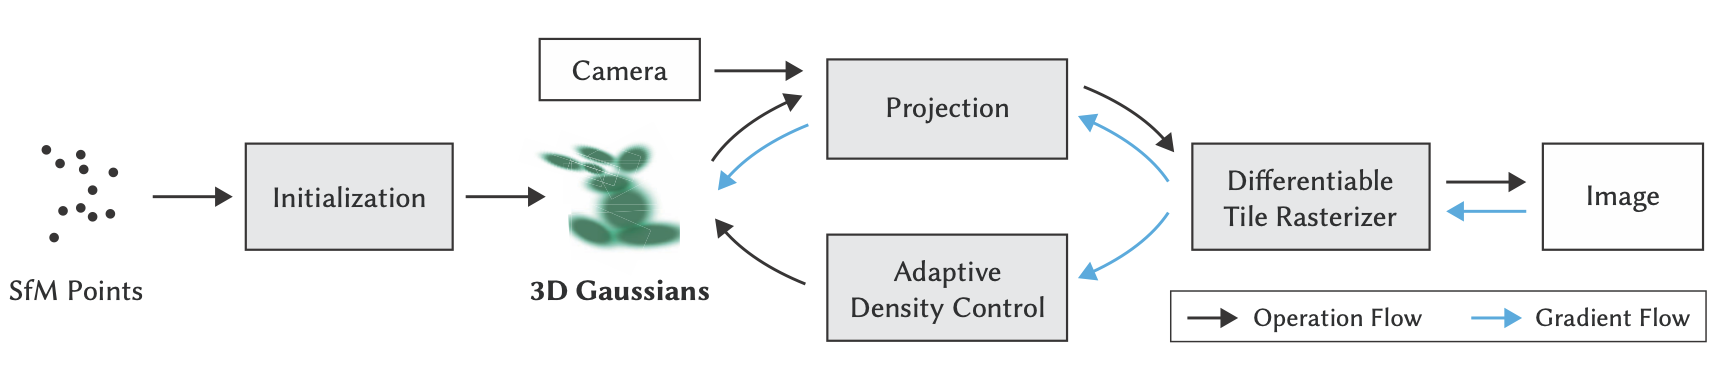
\includegraphics[width=\textwidth]{3DGSWorkflow.png}
    \caption{Overview of the 3D Gaussian Splatting pipeline. The workflow illustrates scene initialization, Gaussian optimization, and real-time rendering via splatting and alpha compositing. Image reproduced from the original 3D Gaussian Splatting paper by Kerbl et al.~\cite{kerbl20233dgs}.}
    \label{fig:3dgs_workflow}
\end{figure}

\subsection{Gaussian Representation}

A scene is represented as a set of $N$ Gaussians:

\[
\mathcal{G} = \{ G_i \}_{i=1}^{N}
\]

Each Gaussian $G_i$ is defined by:

\[
G_i = (\boldsymbol{\mu}_i, \boldsymbol{\Sigma}_i, \alpha_i, \mathbf{c}_i)
\]

where:
\begin{itemize}
    \item $\boldsymbol{\mu}_i \in \mathbb{R}^3$ is the 3D mean (center),
    \item $\boldsymbol{\Sigma}_i \in \mathbb{R}^{3 \times 3}$ is the covariance matrix,
    \item $\alpha_i \in [0,1]$ is the opacity,
    \item $\mathbf{c}_i$ are color coefficients (typically spherical harmonics).
\end{itemize}

The spatial density of a Gaussian is defined as:

\[
\mathcal{N}(\mathbf{x}; \boldsymbol{\mu}_i, \boldsymbol{\Sigma}_i)
=
\exp \left(
-\frac{1}{2}
(\mathbf{x} - \boldsymbol{\mu}_i)^\top
\boldsymbol{\Sigma}_i^{-1}
(\mathbf{x} - \boldsymbol{\mu}_i)
\right).
\]

\subsection{Projection and Rendering}

For a camera with projection function $\pi(\cdot)$, each 3D Gaussian is projected into image space. Due to perspective projection, the Gaussian remains Gaussian in 2D with projected mean and covariance:

\[
\mathbf{u}_i = \pi(\boldsymbol{\mu}_i)
\]

The rendered color at pixel $\mathbf{u}$ is computed using alpha compositing:

\[
C(\mathbf{u}) = \sum_{i} T_i(\mathbf{u}) \alpha_i(\mathbf{u}) \mathbf{c}_i,
\]

where the accumulated transmittance is:

\[
T_i(\mathbf{u}) = \prod_{j < i} \left(1 - \alpha_j(\mathbf{u}) \right).
\]

The Gaussians are sorted in front-to-back order according to depth.

\subsection{Optimization Objective}

The parameters of all Gaussians are optimized by minimizing a photometric reconstruction loss between rendered and ground-truth images:

\[
\mathcal{L}_{rgb}
=
\sum_{\mathbf{u}}
\| C(\mathbf{u}) - I_{gt}(\mathbf{u}) \|_1.
\]

Additional regularization terms such as depth consistency or normal consistency can be incorporated:

\[
\mathcal{L}_{total}
=
\mathcal{L}_{rgb}
+
\lambda_{depth} \mathcal{L}_{depth}
+
\lambda_{normal} \mathcal{L}_{normal}.
\]

\subsection{Adaptive Densification}

To increase representational capacity in complex regions, 3DGS performs adaptive densification. A Gaussian is split when the magnitude of the gradient with respect to its center exceeds a threshold:

\[
\| \nabla_{\boldsymbol{\mu}_i} \mathcal{L}_{total} \| > \gamma.
\]

This mechanism increases the number of Gaussians in high-frequency regions such as edges or textured areas while keeping flat regions compact.

\subsection{Advantages}

Compared to neural radiance fields, 3D Gaussian Splatting:
\begin{itemize}
    \item Enables real-time rendering,
    \item Uses explicit geometric primitives,
    \item Avoids expensive volumetric ray marching,
    \item Allows adaptive refinement through splitting and pruning.
\end{itemize}


\section{Geometry Priors in Gaussian Splatting}
\label{sec:geometry_priors}

While 3D Gaussian Splatting provides an explicit and efficient scene representation, its optimization is primarily driven by photometric supervision. Purely image-based supervision can lead to geometric artifacts such as floaters, inconsistent surface orientation, and poor reconstruction in textureless regions. To address these limitations, additional geometric priors can be incorporated into the training process. These priors introduce structural constraints that improve geometric consistency and stability.

\subsection{Depth Priors}

Depth priors provide direct supervision on scene geometry. Depth information can be obtained from multi-view stereo (MVS) methods, LiDAR sensors, or monocular depth estimation networks.

Let $D_{render}(\mathbf{u})$ denote the depth rendered from the Gaussian representation and $D_{prior}(\mathbf{u})$ the externally estimated depth map. A common supervision term is defined as:

\begin{equation}
\mathcal{L}_{depth}
=
\sum_{\mathbf{u} \in \Omega}
\left|
D_{render}(\mathbf{u}) - D_{prior}(\mathbf{u})
\right|,
\end{equation}

where $\Omega$ represents the set of pixels with reliable depth values.

Depth supervision improves geometric accuracy, reduces floating artifacts, and stabilizes optimization in low-texture regions. However, noisy depth estimates must often be filtered using geometric verification or confidence masks.

\subsection{Normal Priors}

Surface normal priors enforce orientation consistency of reconstructed surfaces. Normals can be derived from depth maps or predicted using monocular normal estimation networks.

Let $\mathbf{n}_{render}(\mathbf{u})$ denote the normal estimated from the rendered Gaussian surface and $\mathbf{n}_{prior}(\mathbf{u})$ the reference normal. A cosine similarity loss is commonly used:

\begin{equation}
\mathcal{L}_{normal}
=
\sum_{\mathbf{u}}
\left(
1 - 
\mathbf{n}_{render}(\mathbf{u})^\top
\mathbf{n}_{prior}(\mathbf{u})
\right).
\end{equation}

Normal constraints improve local surface smoothness and reduce geometric noise, particularly in planar or weakly textured regions.

\subsection{Mesh-Based Priors}

When an approximate surface mesh is available (e.g., reconstructed from MVS), it can serve as a geometric regularizer. Gaussians can be constrained to remain close to the mesh surface.

Let $\mathcal{M}$ denote a reference mesh and $\text{dist}(\boldsymbol{\mu}_i, \mathcal{M})$ the shortest distance from a Gaussian center to the mesh surface. A regularization term can be defined as:

\begin{equation}
\mathcal{L}_{mesh}
=
\sum_{i}
\text{dist}(\boldsymbol{\mu}_i, \mathcal{M})^2.
\end{equation}

This prior enforces surface adherence and improves global geometric consistency. It is particularly useful in structured environments where reliable coarse geometry can be extracted.

\subsection{Edge and Line Priors}

Image edges and line segments encode strong structural cues about scene geometry. Line detection methods can extract 2D line segments, which can be matched across views to recover 3D line constraints.

Let $\mathbf{l}_{render}$ denote projected Gaussian-induced edges and $\mathbf{l}_{obs}$ detected image lines. An alignment loss may penalize angular deviation or distance between projected and observed lines:

\begin{equation}
\mathcal{L}_{edge}
=
\sum_{k}
\left\|
\mathbf{l}_{render}^{(k)} -
\mathbf{l}_{obs}^{(k)}
\right\|.
\end{equation}

Edge-based priors improve reconstruction of sharp structures such as building edges, corners, and object boundaries, which are often smoothed by purely photometric optimization.

Incorporating geometric priors transforms Gaussian Splatting from a purely photometric renderer into a geometry-aware representation capable of producing structurally consistent reconstructions.



\section{Quality Metrics}
\label{sec:quality_metrics}

To quantitatively evaluate the visual quality of the reconstructed images, we employ several commonly used image quality metrics: Peak Signal-to-Noise Ratio (PSNR), Structural Similarity Index Measure (SSIM), and Learned Perceptual Image Patch Similarity (LPIPS). These metrics capture complementary aspects of reconstruction quality, ranging from pixel-wise accuracy to perceptual similarity, and are widely adopted in neural rendering and view synthesis literature~\cite{mildenhall2020nerf,kerbl20233dgs}.

\subsection{Peak Signal-to-Noise Ratio (PSNR)}

Peak Signal-to-Noise Ratio (PSNR) is a pixel-wise fidelity metric that measures the difference between a reconstructed image and the corresponding ground truth image. It is derived from the Mean Squared Error (MSE) and is expressed in decibels (dB). Higher PSNR values indicate better reconstruction quality and lower pixel-wise reconstruction error.

Given a ground truth image $I$ and a reconstructed image $\hat{I}$ of size $H \times W$, the MSE is defined as:
\begin{equation}
\mathrm{MSE} = \frac{1}{HW} \sum_{i=1}^{H} \sum_{j=1}^{W} \left( I(i,j) - \hat{I}(i,j) \right)^2
\end{equation}

PSNR is then computed as:
\begin{equation}
\mathrm{PSNR} = 10 \cdot \log_{10} \left( \frac{L^2}{\mathrm{MSE}} \right)
\end{equation}
where $L$ denotes the maximum possible pixel value (e.g., $L = 255$ for 8-bit images).

PSNR is commonly used in image reconstruction tasks due to its simplicity, but it does not always correlate well with perceived visual quality~\cite{wang2004ssim}.

\subsection{Structural Similarity Index Measure (SSIM)}

Structural Similarity Index Measure (SSIM) evaluates image quality by comparing structural information between the reconstructed and ground truth images. Unlike PSNR, SSIM explicitly models perceptual factors by decomposing image similarity into luminance, contrast, and structural components~\cite{wang2004ssim}.

SSIM between images $I$ and $\hat{I}$ is defined as:
\begin{equation}
\mathrm{SSIM}(I, \hat{I}) =
\frac{(2 \mu_I \mu_{\hat{I}} + C_1)(2 \sigma_{I\hat{I}} + C_2)}
{(\mu_I^2 + \mu_{\hat{I}}^2 + C_1)(\sigma_I^2 + \sigma_{\hat{I}}^2 + C_2)}
\end{equation}

where:
\begin{itemize}
    \item $\mu_I$, $\mu_{\hat{I}}$ are the mean intensities of the images,
    \item $\sigma_I^2$, $\sigma_{\hat{I}}^2$ are the variances,
    \item $\sigma_{I\hat{I}}$ is the covariance between $I$ and $\hat{I}$,
    \item $C_1$ and $C_2$ are small constants added for numerical stability.
\end{itemize}

SSIM values range from $-1$ to $1$, with higher values indicating greater structural similarity. In practice, SSIM is often computed over local windows and averaged across the image to better capture spatially varying distortions.

\subsection{Learned Perceptual Image Patch Similarity (LPIPS)}

Learned Perceptual Image Patch Similarity (LPIPS) is a perceptual metric designed to better align with human visual judgments. Instead of relying on pixel-wise differences, LPIPS measures the distance between deep feature representations extracted from pretrained convolutional neural networks~\cite{zhang2018lpips}.

Given feature activations $\phi_l(I)$ and $\phi_l(\hat{I})$ from layer $l$ of a pretrained network, LPIPS is computed as:
\begin{equation}
\mathrm{LPIPS}(I, \hat{I}) =
\sum_{l} \frac{1}{H_l W_l}
\sum_{h,w} \left\| w_l \odot
\left( \phi_l(I)_{h,w} - \phi_l(\hat{I})_{h,w} \right) \right\|_2^2
\end{equation}

where:
\begin{itemize}
    \item $\phi_l(\cdot)$ denotes feature maps at layer $l$,
    \item $w_l$ are learned channel-wise weights,
    \item $H_l$ and $W_l$ are spatial dimensions of the feature map,
    \item $\odot$ denotes element-wise multiplication.
\end{itemize}

Lower LPIPS values indicate higher perceptual similarity between images. Due to its strong correlation with human perception, LPIPS is widely used to evaluate visual quality in neural rendering and view synthesis tasks~\cite{kerbl20233dgs,mildenhall2020nerf}.

\chapter{Proposed Solution}

\section{Problem Formulation}

Let $\mathcal{I} = \{I_i\}_{i=1}^N$ be a set of calibrated multi-view images with known camera poses obtained from Structure-from-Motion.
The goal is to reconstruct a geometrically consistent scene representation using a set of Gaussian primitives:

\begin{equation}
\mathcal{G} = \{ g_k \}_{k=1}^K,
\end{equation}

where each Gaussian $g_k$ is parameterized by its center $\mathbf{x}_k \in \mathbb{R}^3$, covariance $\Sigma_k$, opacity $\alpha_k$, and color features.

The standard 3D Gaussian Splatting formulation optimizes parameters by minimizing photometric reconstruction error:

\begin{equation}
\mathcal{L}_{photo} =
\sum_{i=1}^{N}
\left\|
R(\mathcal{G}, \Pi_i) - I_i
\right\|_2^2,
\end{equation}

where $R(\cdot)$ denotes the differentiable renderer and $\Pi_i$ is the projection associated with camera $i$.

However, purely photometric supervision is insufficient in:

\begin{itemize}
    \item textureless planar regions,
    \item areas with weak gradients,
    \item geometrically ambiguous boundaries.
\end{itemize}

This often leads to over-densification, floating artifacts, and inconsistent surface normals.

To address these limitations, we introduce geometry-aware regularization and adaptive primitive allocation into the optimization process.

The final objective becomes:

\begin{equation}
\mathcal{L} =
\mathcal{L}_{photo}
+
\lambda_d \mathcal{L}_{depth}
+
\lambda_n \mathcal{L}_{normal}
+
\lambda_p \mathcal{L}_{planar}
+
\lambda_e \mathcal{L}_{edge},
\end{equation}

\noindent where $\lambda_d$ weights the depth prior described in Section~\ref{sec:depth_prior}, $\lambda_n$ weights the normal prior described in Section~\ref{sec:normal_prior}, $\lambda_p$ weights the planar regularization described in Section~\ref{sec:planar_prior}, and $\lambda_e$ weights the edge-aware normal reinforcement described in Section~\ref{sec:edge_prior}.

\section{Geometric Prior Formulations}
\label{sec:geometry_priors}

While 3D Gaussian Splatting provides an explicit and efficient scene representation, its optimization is primarily driven by photometric supervision. Purely image-based supervision can lead to geometric artifacts such as floaters, inconsistent surface orientation, and poor reconstruction in textureless regions. To address these limitations, additional geometric priors are incorporated into the training process. This section introduces the general form of each prior type; their specific implementation within our framework is described in Section~\ref{sec:solution_architecture}.

\subsection{Depth Priors}

Depth priors provide direct supervision on scene geometry. Depth information can be obtained from multi-view stereo (MVS) methods, LiDAR sensors, or monocular depth estimation networks. Let $D_{render}(\mathbf{u})$ denote the depth rendered from the Gaussian representation and $D_{prior}(\mathbf{u})$ the externally estimated depth map. A common supervision term is:

\begin{equation}
\mathcal{L}_{depth}
=
\sum_{\mathbf{u} \in \Omega}
\left|
D_{render}(\mathbf{u}) - D_{prior}(\mathbf{u})
\right|,
\end{equation}

where $\Omega$ is the set of pixels with reliable depth values. Depth supervision reduces floating artifacts and stabilizes optimization in low-texture regions.

\subsection{Normal Priors}

Surface normal priors enforce orientation consistency of reconstructed surfaces. Normals can be derived from depth maps or predicted by monocular estimation networks. Let $\mathbf{n}_{render}(\mathbf{u})$ denote the rendered surface normal and $\mathbf{n}_{prior}(\mathbf{u})$ the reference normal. A cosine-similarity loss is commonly used:

\begin{equation}
\mathcal{L}_{normal}
=
\sum_{\mathbf{u}}
\left(
1 -
\mathbf{n}_{render}(\mathbf{u})^\top
\mathbf{n}_{prior}(\mathbf{u})
\right).
\end{equation}

Normal constraints improve local surface smoothness and reduce geometric noise, particularly in planar or weakly textured regions.

\subsection{Mesh-Based Priors}

When an approximate surface mesh $\mathcal{M}$ is available (e.g., reconstructed via TSDF fusion), it can serve as a geometric regularizer. Let $\text{dist}(\boldsymbol{\mu}_i, \mathcal{M})$ denote the shortest distance from the $i$-th Gaussian center to the mesh surface. The regularization term is:

\begin{equation}
\mathcal{L}_{mesh}
=
\sum_{i}
\text{dist}(\boldsymbol{\mu}_i, \mathcal{M})^2.
\end{equation}

This prior enforces surface adherence and improves global geometric consistency, and is particularly useful in structured environments where reliable coarse geometry can be extracted.

\subsection{Edge and Planar Priors}

Image edges and planar segment boundaries encode strong structural cues. Planar priors encourage Gaussians within a detected plane to share a common depth surface. Edge-aware priors spatially modulate primitive allocation: densification is boosted near structural boundaries and suppressed in homogeneous interiors. Together, these priors improve reconstruction of sharp transitions and prevent over-densification on large flat surfaces.

\section{Solution Architecture}
\label{sec:solution_architecture}

Figure~\ref{fig:unified_pipeline} presents the overall architecture of the proposed framework. The pipeline takes a set of calibrated multi-view images as input and extracts four monocular geometric priors — edges derived from plane boundaries, plane segmentation masks, dense depth maps, and surface normal maps — each of which feeds into a corresponding rendering-space loss term. These four loss terms, together with the standard photometric loss $\mathcal{L}_{rgb}$ and an optional mesh-based term $\mathcal{L}_{mesh}$, are jointly minimized during Gaussian optimization. The diagram uses color coding to distinguish component types: blue boxes represent input geometric priors, green boxes denote loss regularization terms, purple boxes indicate processing steps, and orange represents the central optimization objective.

\begin{figure}[t]
    \centering
    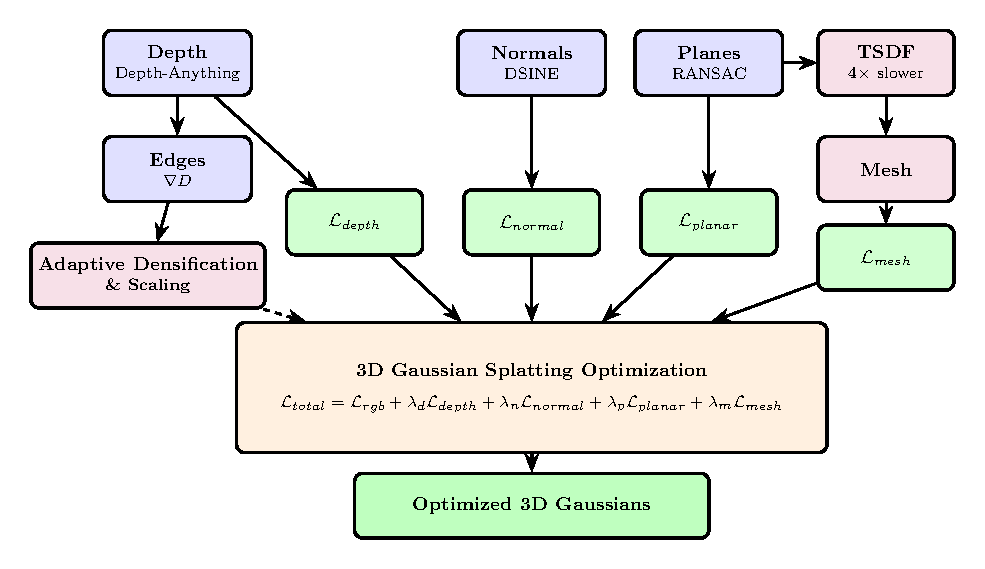
\includegraphics[width=\linewidth]{pipeline_unified.pdf}
    \caption{Unified geometry-aware 3D Gaussian Splatting framework.}
    \label{fig:unified_pipeline}
\end{figure}

The architecture extends the standard Gaussian Splatting pipeline with two complementary components:

\begin{enumerate}
    \item Geometry-aware priors operating in rendering space.
    \item Edge-aware adaptive densification for compact representation.
\end{enumerate}

\subsection{Geometry-Aware Regularization}

All geometric constraints are applied in rendering space rather than directly constraining primitive parameters. This preserves the flexibility of Gaussian primitives while enforcing global geometric consistency.

\subsubsection{Depth Prior}
\label{sec:depth_prior}

Depth prior maps $D_p$ are estimated per-view using DUST3R (Dense Unsupervised Surface Transformation via Regression), a fast monocular depth estimator. These priors are aligned with rendered depth $D_r$ to stabilize optimization in textureless regions:

\begin{equation}
\mathcal{L}_{depth}
=
\left\|
D_r - D_p
\right\|_1,
\end{equation}

reducing floating artifacts and improving geometric consistency across views.

\subsubsection{Normal Prior}
\label{sec:normal_prior}

Surface normal prior maps $N_p$ are also estimated using DUST3R per-view. These normals are regularized alongside rendered normals $N_r$:

\begin{equation}
\mathcal{L}_{normal}
=
\left\|
N_r - N_p
\right\|_1
+
\left(1 - N_r \cdot N_p \right),
\end{equation}

promoting locally coherent surface orientation and reducing normal inconsistencies.

\subsubsection{Planar Regularization}
\label{sec:planar_prior}

Planar segmentation priors are extracted from single images using SAM3 (Segment Anything Model v3), which identifies and delineates planar regions. For each segmented planar region, a plane is fitted to the rendered depth map. Let $D_{plane}$ denote the depth values induced by this fitted plane. The planar consistency loss is:

\begin{equation}
\mathcal{L}_{planar}
=
\left\|
D_r - D_{plane}
\right\|_1.
\end{equation}

Importantly, Gaussian centers are not explicitly projected onto planes; the constraint operates purely at the rendering level, allowing primitives to reorganize naturally during optimization.

Figure~\ref{fig:planar_segmentation} illustrates the planar segmentation applied to a DrJohnson training view. The left subfigure shows the output of SAM3, where each color-coded region corresponds to one detected plane. The right subfigure shows the extracted plane boundaries, which define the spatial extent of the co-planarity constraint. These boundaries are later reused in the edge-aware densification strategy described in Section~\ref{sec:edge_aware}.

\begin{figure}[h]
    \centering
    \begin{subfigure}{0.48\textwidth}
        \centering
        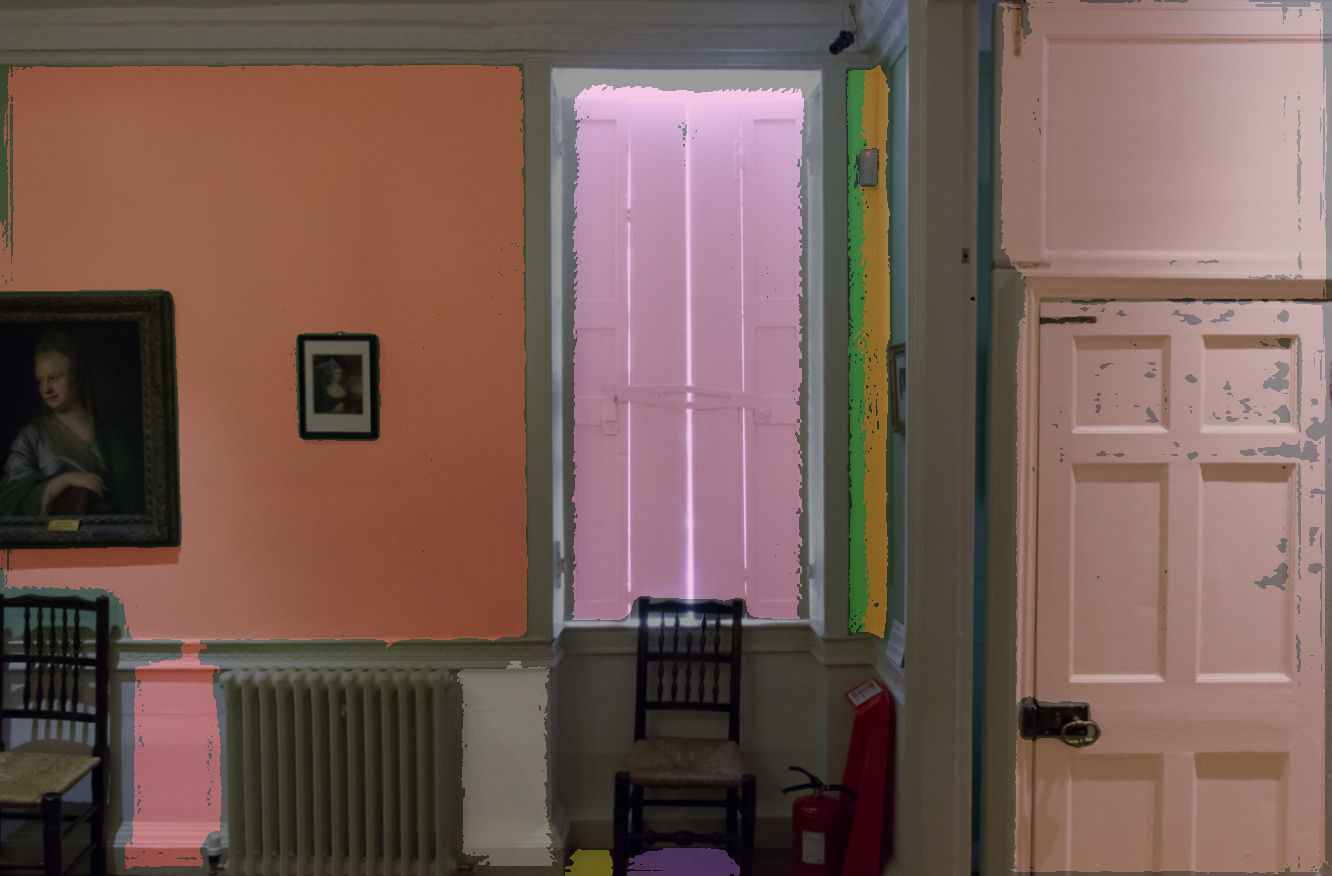
\includegraphics[width=\textwidth]{comparison_figures/planar_mask_overlay.png}
        \caption{Segmented planar regions (each colour = one plane)}
    \end{subfigure}
    \hfill
    \begin{subfigure}{0.48\textwidth}
        \centering
        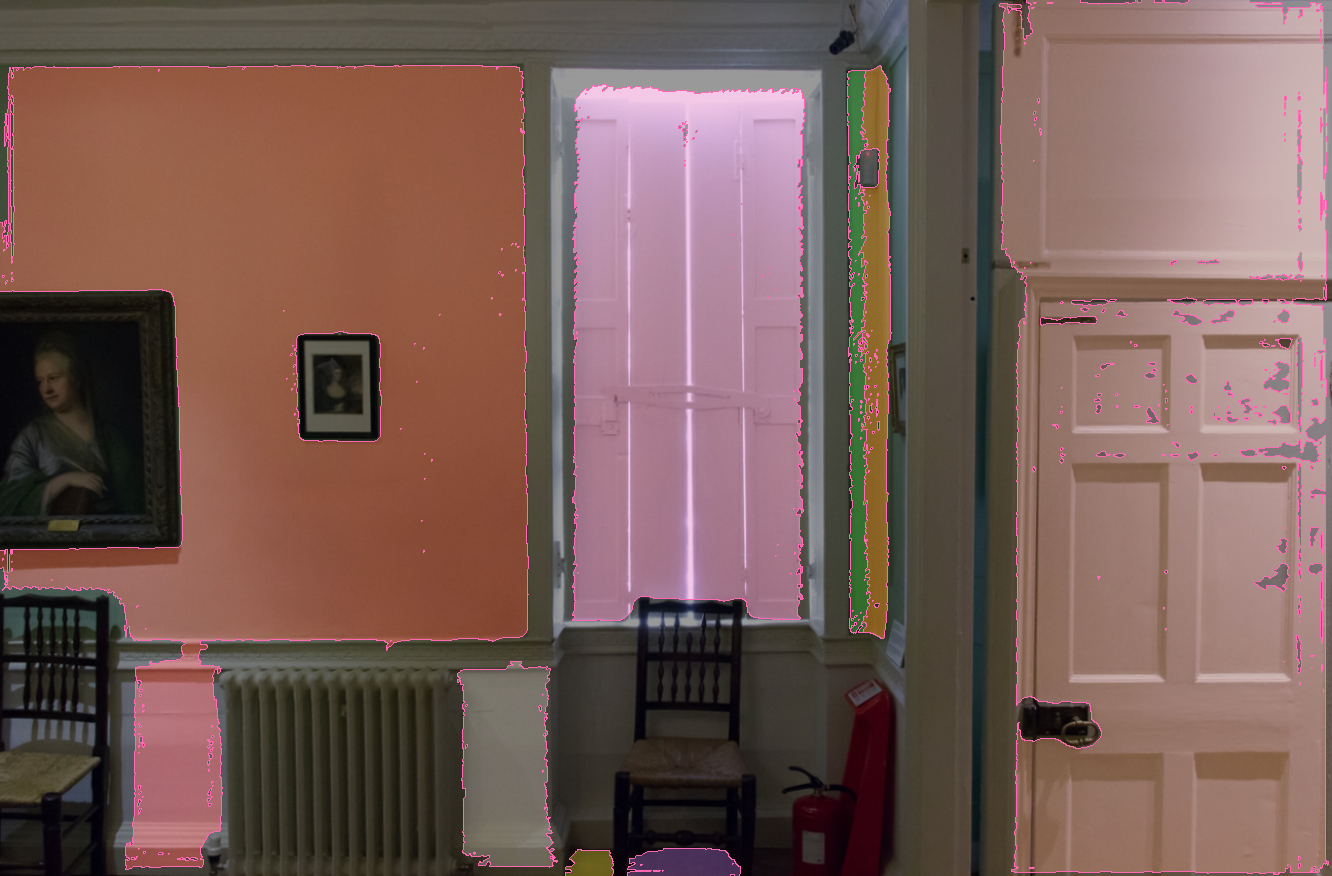
\includegraphics[width=\textwidth]{comparison_figures/plane_boundaries_pink.png}
        \caption{Plane boundaries extracted from segmentation}
    \end{subfigure}
    \caption{Planar segmentation on a DrJohnson training view.}
    \label{fig:planar_segmentation}
\end{figure}

\subsection{Edge-Aware Adaptive Representation}
\label{sec:edge_aware}

In addition to geometric priors, we introduce a spatially adaptive densification mechanism. The core intuition is straightforward: structural boundaries between planes require precise, fine-grained representation, while large homogeneous planar interiors can be covered efficiently with fewer, larger primitives.

Structural edges are identified from SAM3 planar segment boundaries, which naturally encode geometric discontinuities in the scene. Based on each Gaussian's 3D distance to these boundaries, the optimization applies two complementary rules:

\begin{itemize}
    \item \textbf{Near structural edges:} densification is boosted (split probability multiplied by $\times$2.5) and scale is capped small ($s_{\min} = 0.3$), producing many precise, localized Gaussians that capture sharp transitions faithfully.
    \item \textbf{In planar interiors:} densification is suppressed (split probability reduced by $\times$0.4) and Gaussians are free to grow large ($s_{\max} = 2.0$), covering large flat surfaces with far fewer primitives.
\end{itemize}

This allocation strategy concentrates representational capacity exactly where geometric detail is required, while preventing over-densification in uniform regions — the primary mechanism behind the model size reduction achieved by our method.

Figure~\ref{fig:edge_detection} shows the structural edge detection applied to the same DrJohnson training view. The left subfigure overlays the detected plane boundary lines on the original image; the right subfigure shows the resulting structural line segments after post-processing. Gaussians whose 3D centers project close to these lines receive boosted split probability and a tighter scale constraint, while Gaussians in the flat interiors between lines are allowed to grow large and are split less aggressively.

\begin{figure}[h]
    \centering
    \begin{subfigure}{0.48\textwidth}
        \centering
        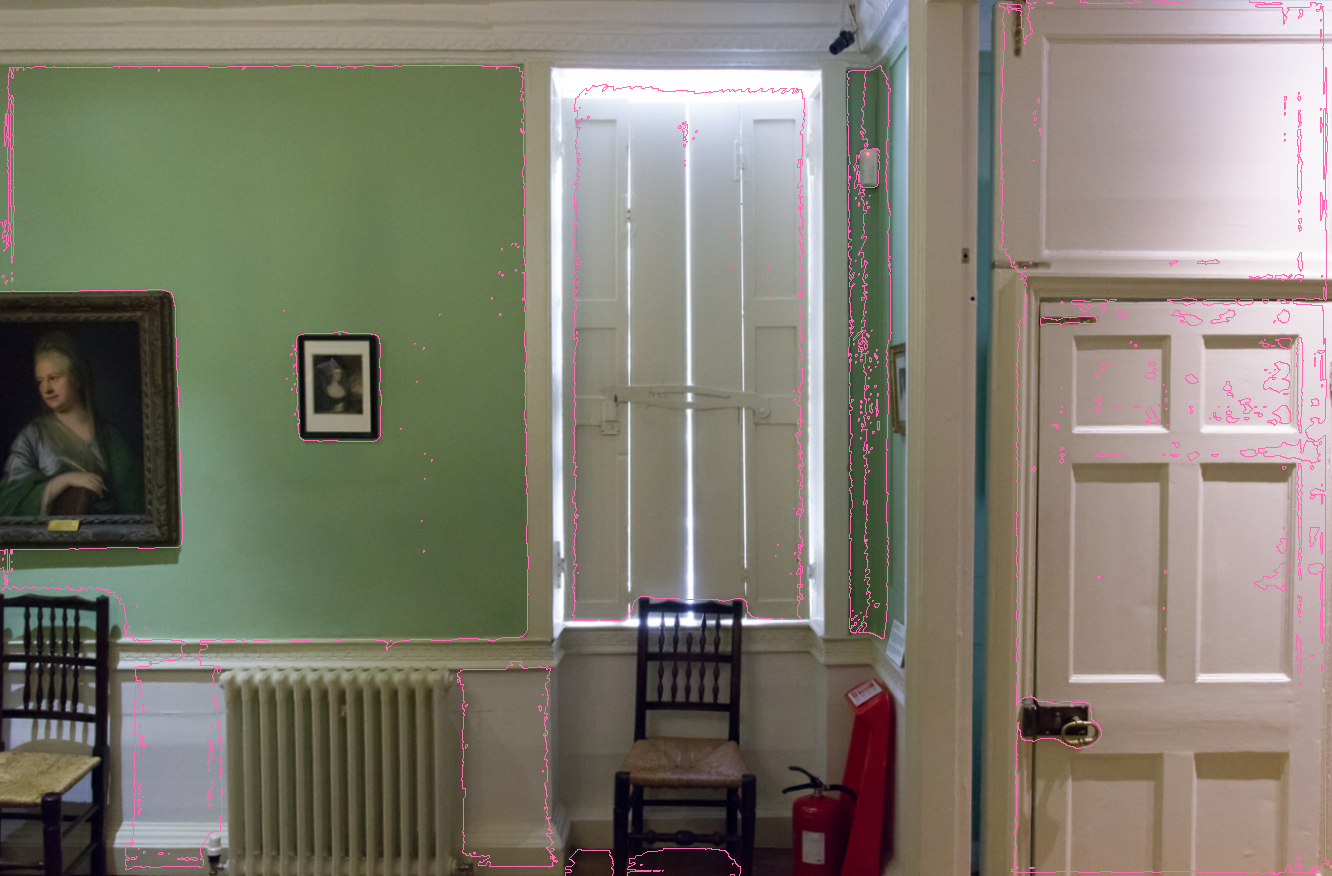
\includegraphics[width=\textwidth]{comparison_figures/edge_boundaries_on_image.png}
        \caption{Plane boundary lines overlaid on scene}
    \end{subfigure}
    \hfill
    \begin{subfigure}{0.48\textwidth}
        \centering
        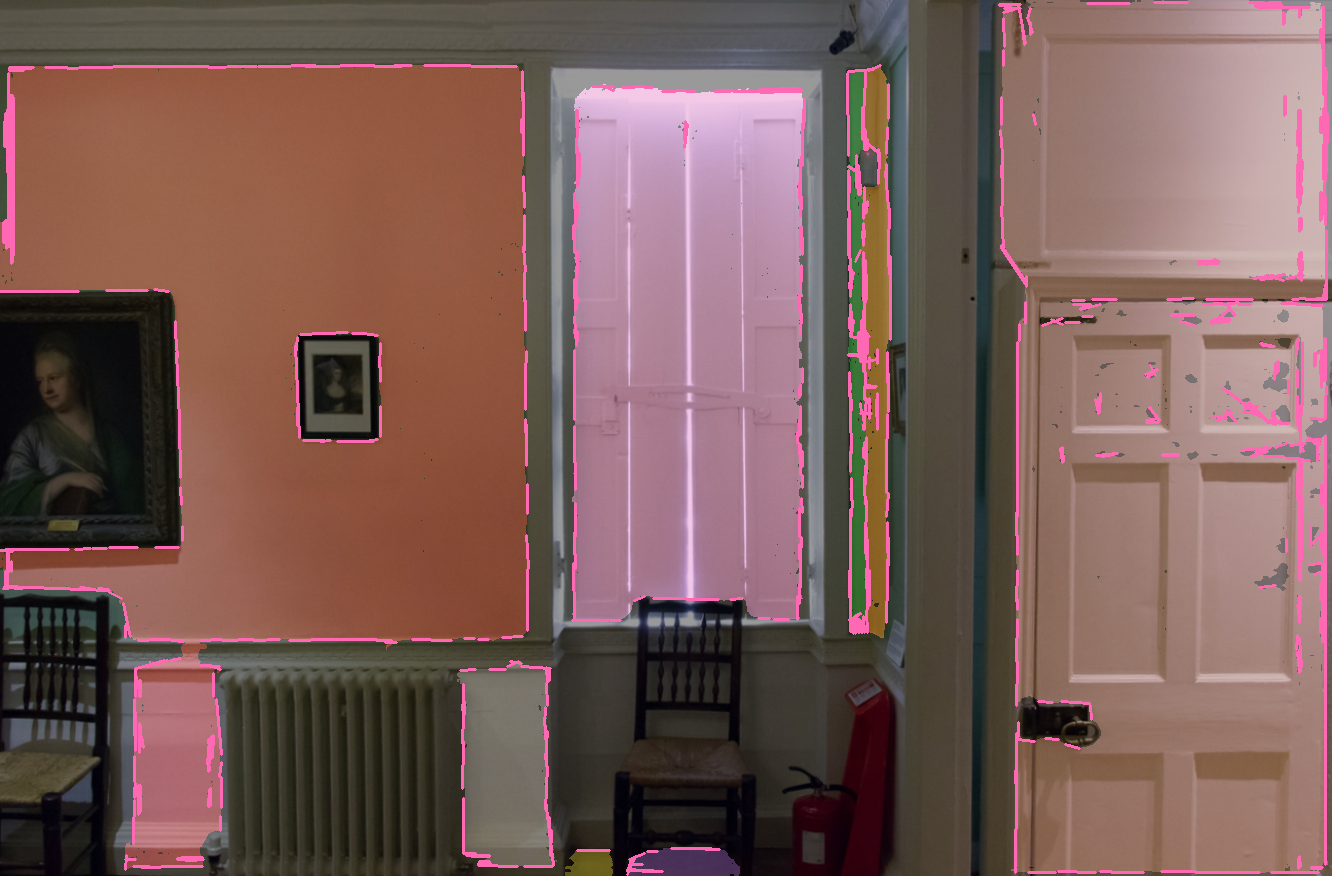
\includegraphics[width=\textwidth]{comparison_figures/edge_extracted_lines.png}
        \caption{Extracted structural line segments}
    \end{subfigure}
    \caption{Structural edge detection on a DrJohnson training view.}
    \label{fig:edge_detection}
\end{figure}

\subsubsection{Edge-Specific Normal Reinforcement}
\label{sec:edge_prior}

Optionally, an additional edge-restricted normal alignment term can be activated:

\begin{equation}
\mathcal{L}_{edge}
=
\left\|
N_r - N_{depth}
\right\|_1
+
\left(1 - N_r \cdot N_{depth} \right).
\end{equation}

This term is applied only at detected edge pixels and introduced after initial geometric stabilization to reinforce sharp transitions.

\section{Solution Summary}

The proposed framework augments standard Gaussian Splatting with:

\begin{itemize}
    \item Rendering-space geometric regularization (depth, normals, planarity),
    \item Edge-aware adaptive densification,
    \item Optional mesh-based TSDF regularization.
\end{itemize}

The design preserves the efficiency and differentiability of the original pipeline while improving geometric consistency, structural sharpness, and representation compactness.

All components are integrated into a unified training framework, enabling systematic evaluation of geometric priors and adaptive primitive allocation within a single optimization process.
 
\chapter{Experiments and Results}

\section{Datasets}

This section describes the data used to evaluate the proposed method. We outline the selected benchmark dataset, the specific scenes considered, and the properties that make them suitable for assessing geometry-aware regularization.

\subsection{Deep Blending Dataset}

We evaluate the proposed method on the Deep Blending dataset~\cite{hedman2018deepblending}, which is widely used in neural rendering research for benchmarking view synthesis and reconstruction quality. The dataset consists of multi-view image sequences with accurately estimated camera poses obtained through Structure-from-Motion pipelines using COLMAP~\cite{schoenberger2016sfm}.

We focus on three indoor scenes from the Deep Blending dataset: \textbf{DrJohnson}, \textbf{Library}, and \textbf{Playroom}. These scenes are characterized by challenging indoor environments with large planar regions, reflective surfaces, and areas with limited texture. Indoor environments are particularly suitable for evaluating geometry-aware priors because they contain dominant planar structures (walls, floors, ceilings, furniture surfaces) that benefit significantly from structural regularization. All quantitative results reported in this chapter represent averages computed across these three scenes unless otherwise specified.

\begin{figure}[h]
    \centering
    \begin{subfigure}{0.32\textwidth}
        \centering
        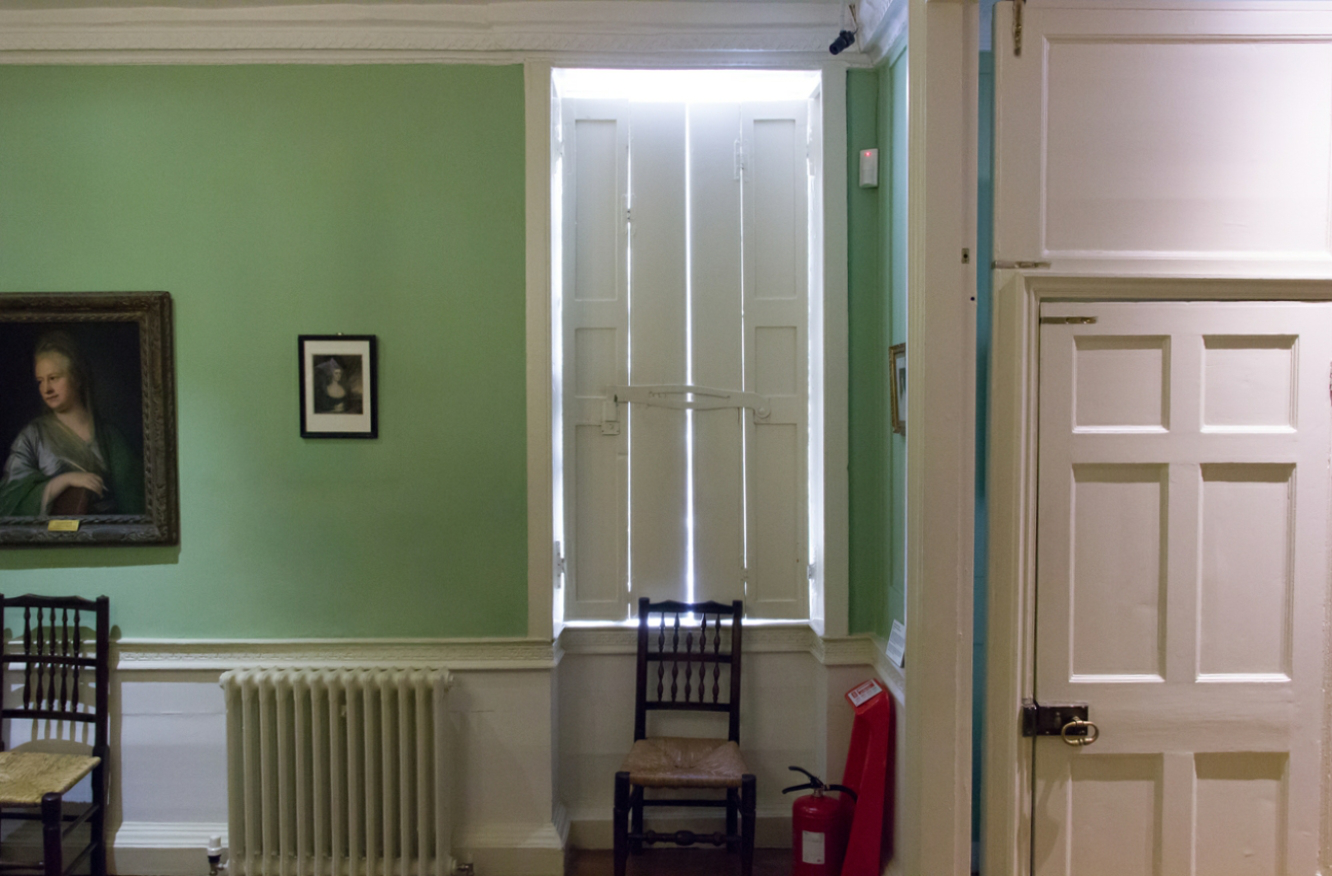
\includegraphics[width=\textwidth]{comparison_figures/drjohnson_gt_view01.png}
        \caption{DrJohnson: green room}
    \end{subfigure}
    \hfill
    \begin{subfigure}{0.32\textwidth}
        \centering
        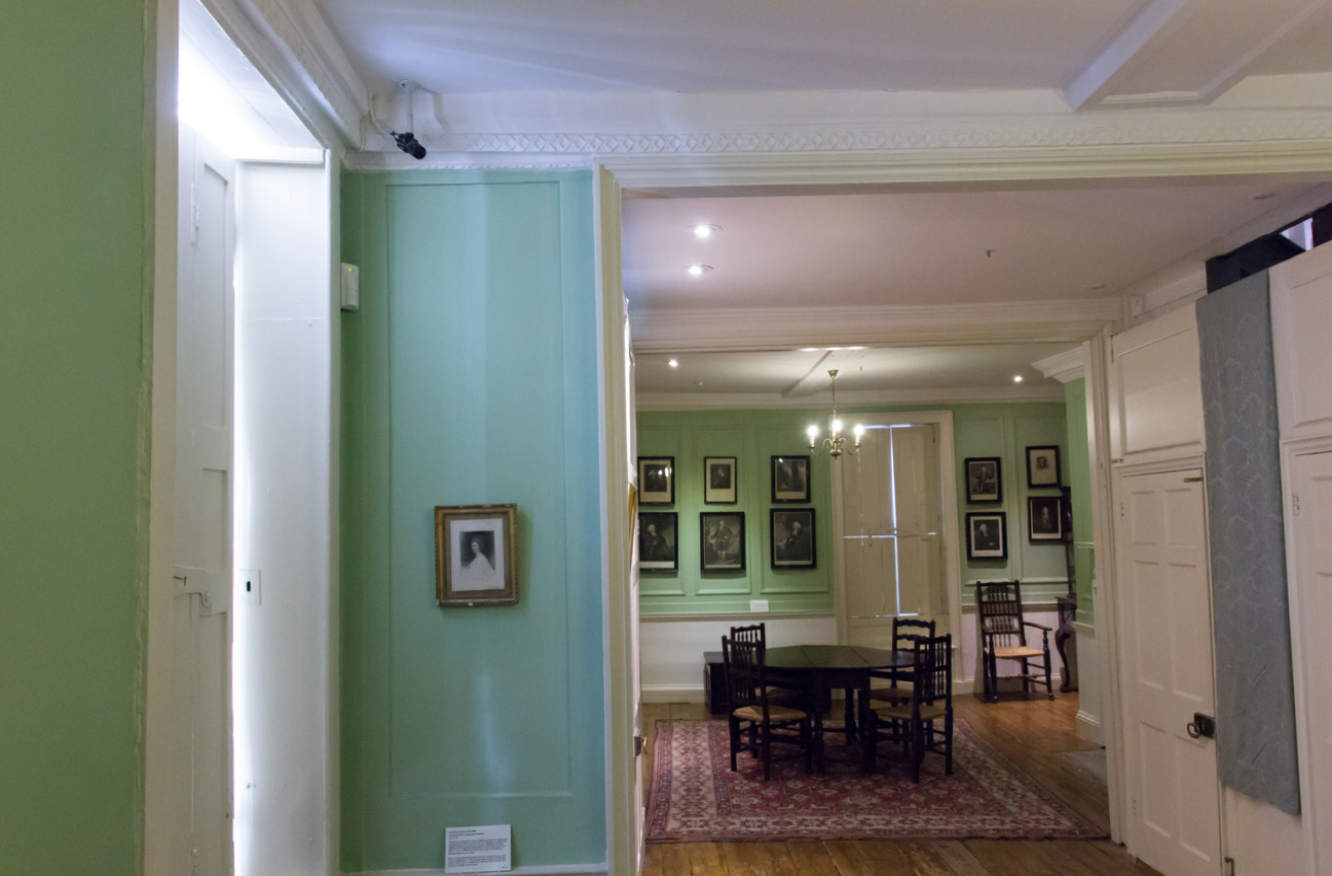
\includegraphics[width=\textwidth]{comparison_figures/drjohnson_gt_view03.png}
        \caption{DrJohnson: hallway}
    \end{subfigure}
    \hfill
    \begin{subfigure}{0.32\textwidth}
        \centering
        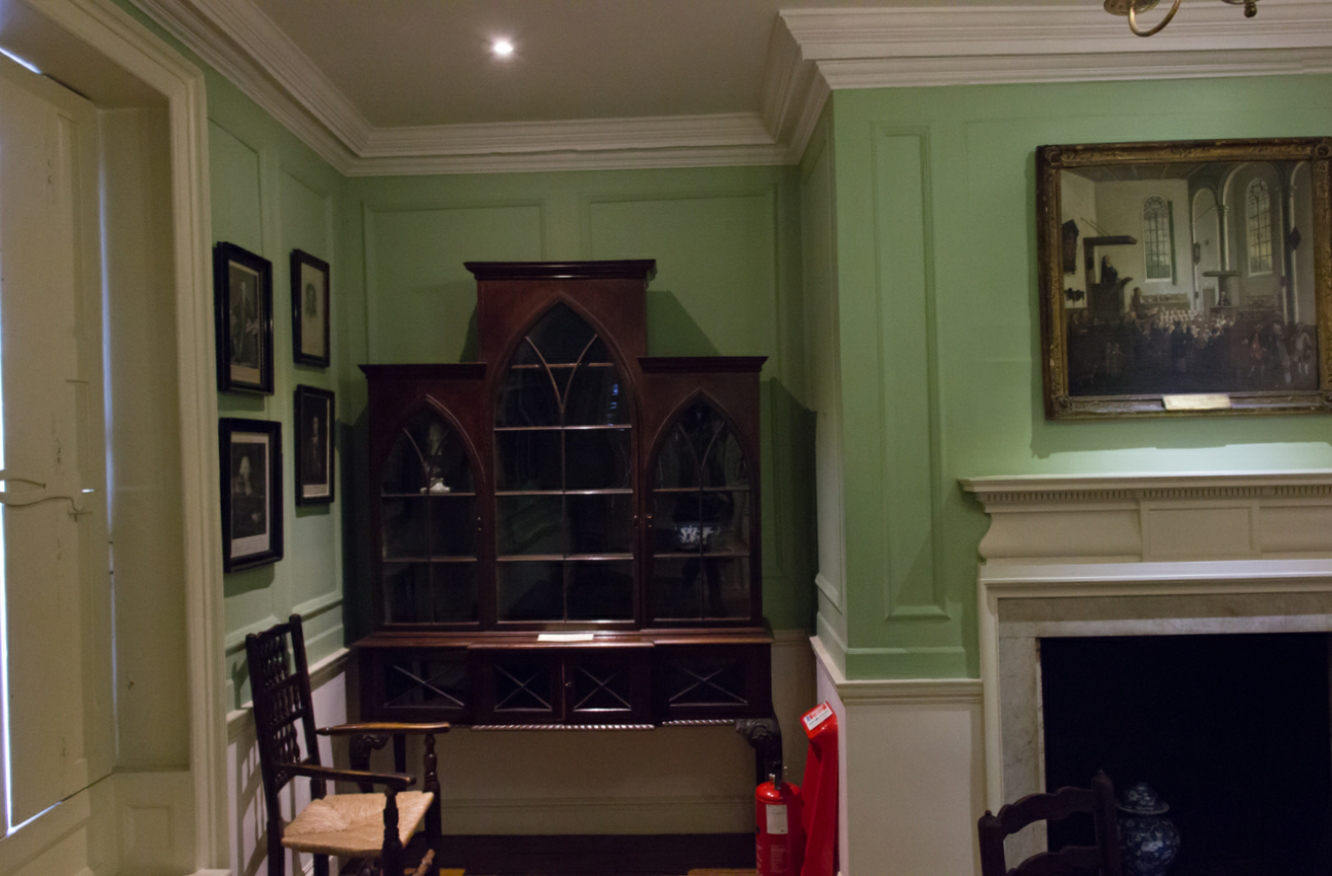
\includegraphics[width=\textwidth]{comparison_figures/drjohnson_gt_view04.png}
        \caption{DrJohnson: cabinet room}
    \end{subfigure}

    \vspace{0.5em}

    \begin{subfigure}{0.48\textwidth}
        \centering
        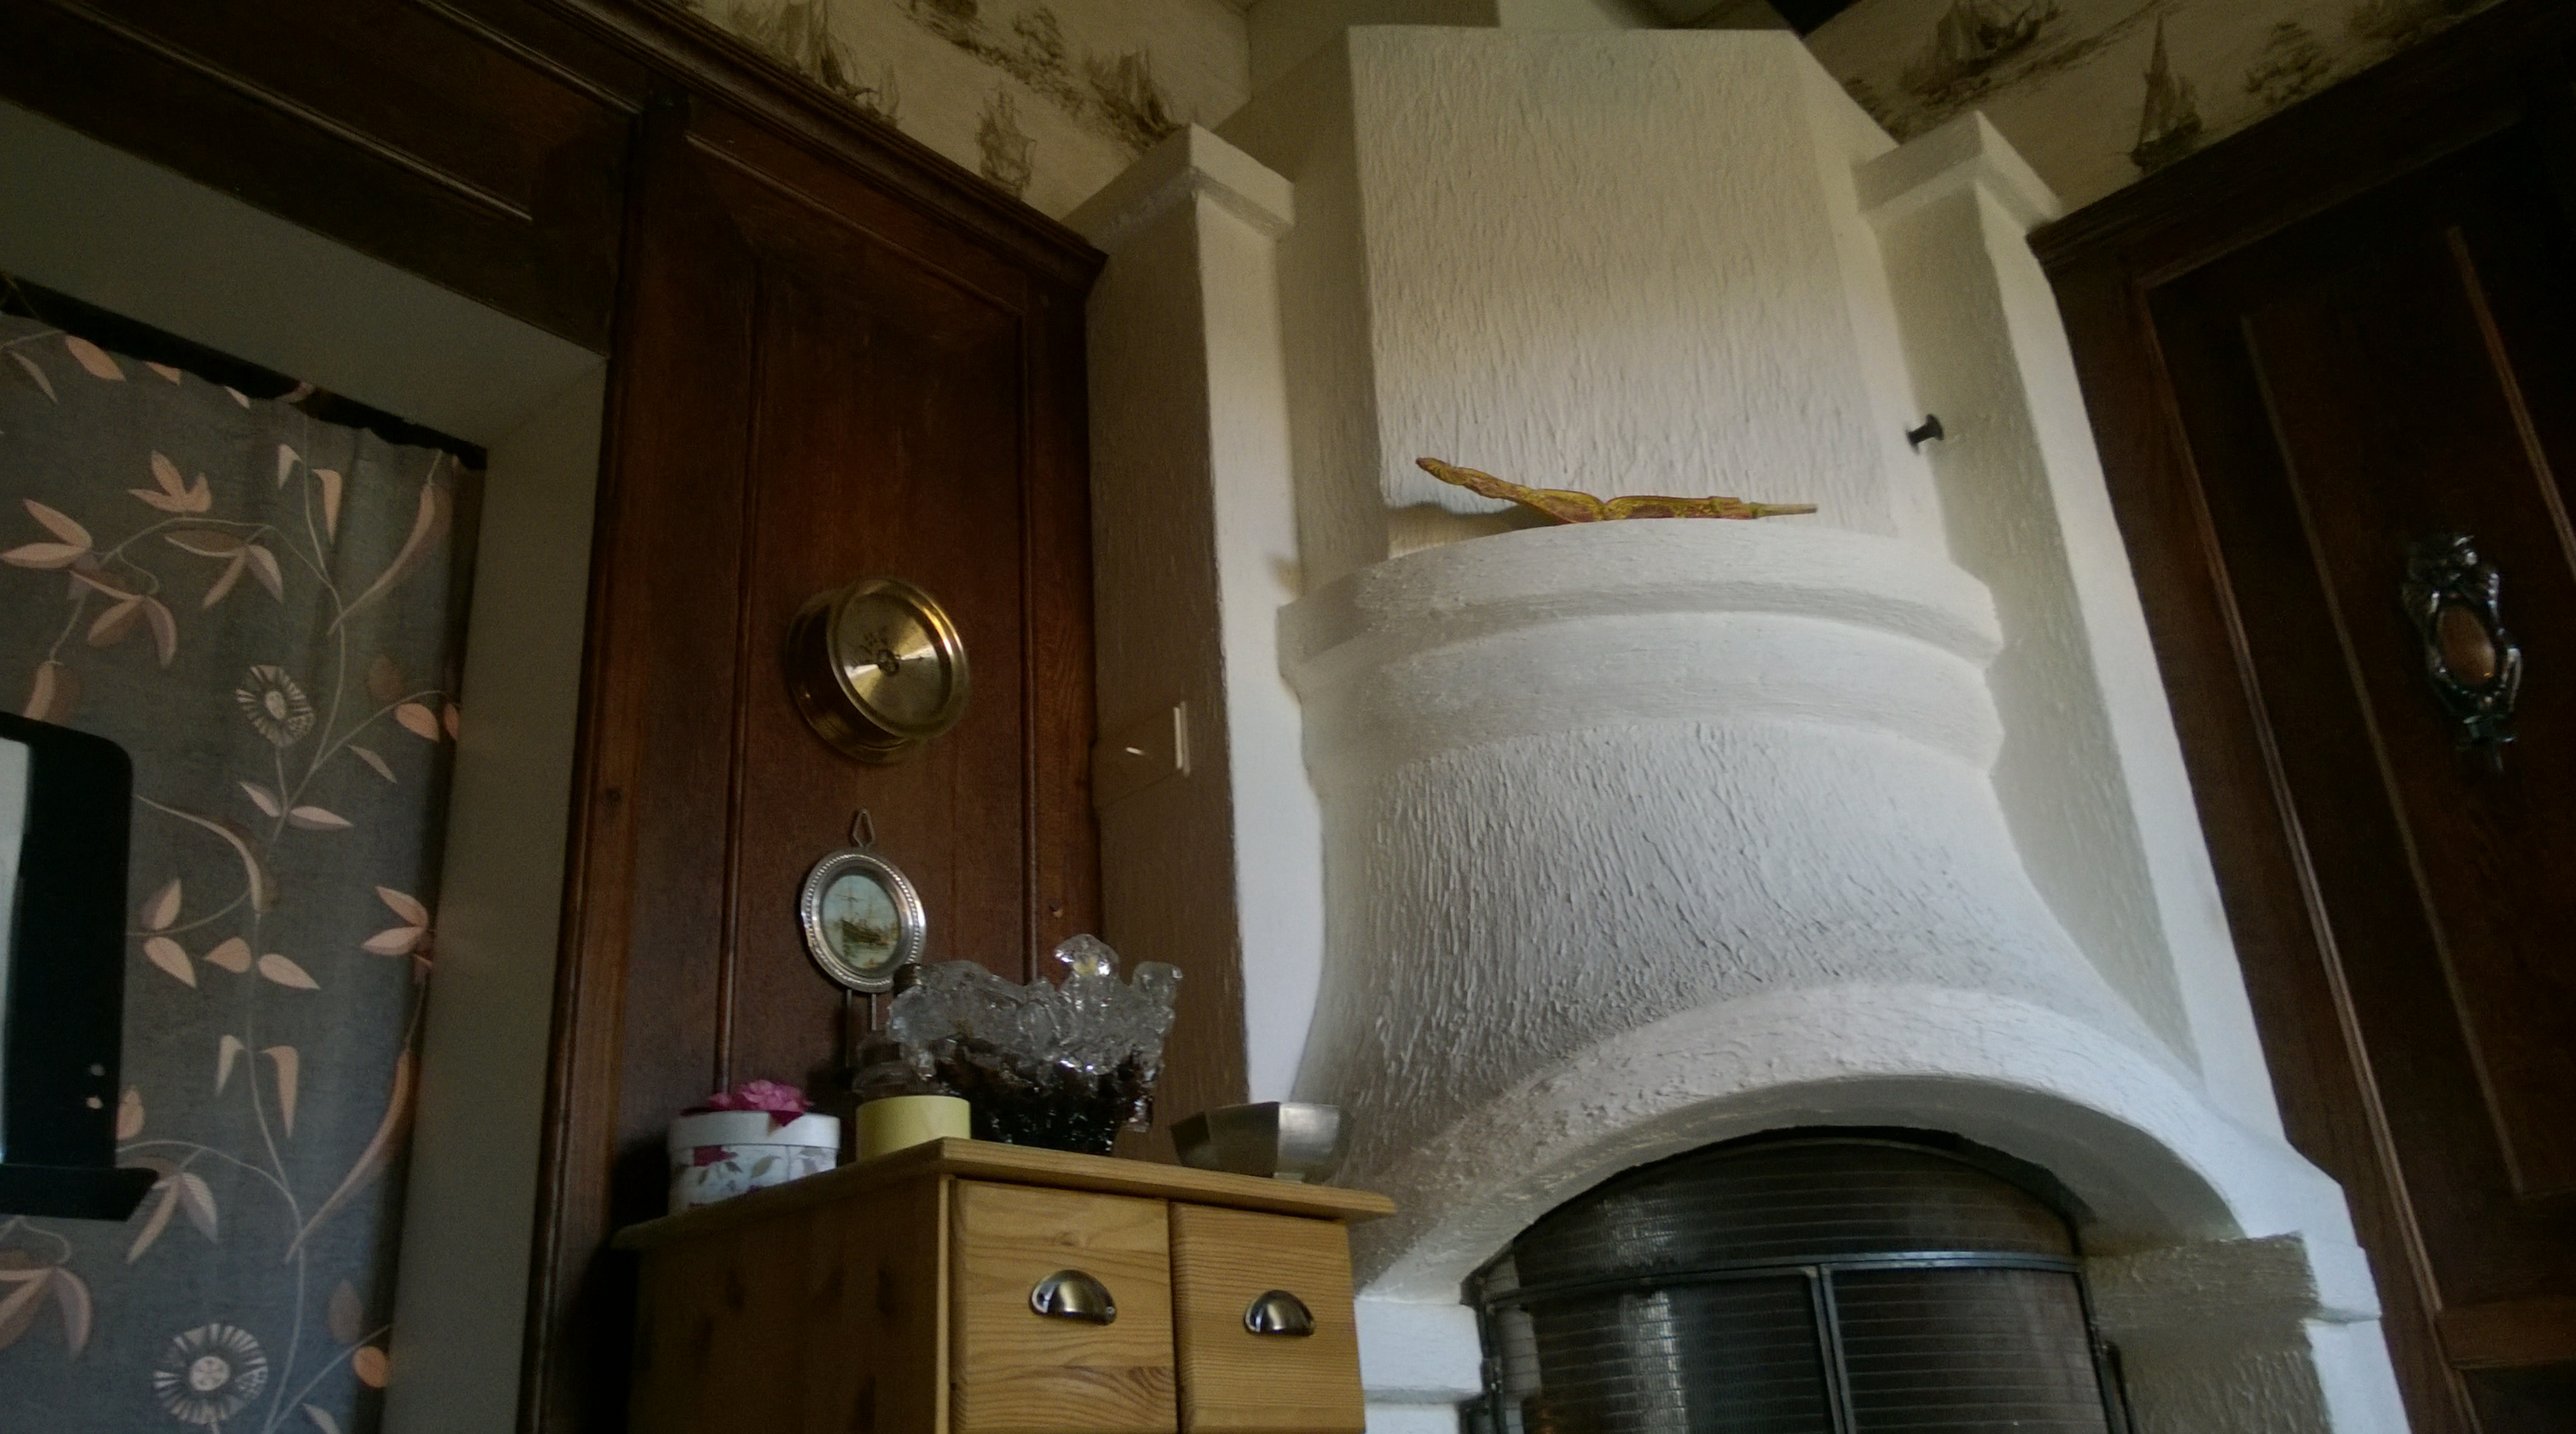
\includegraphics[width=\textwidth]{comparison_figures/library_sample.jpg}
        \caption{Library: wooden furniture and stucco fireplace}
    \end{subfigure}
    \hfill
    \begin{subfigure}{0.48\textwidth}
        \centering
        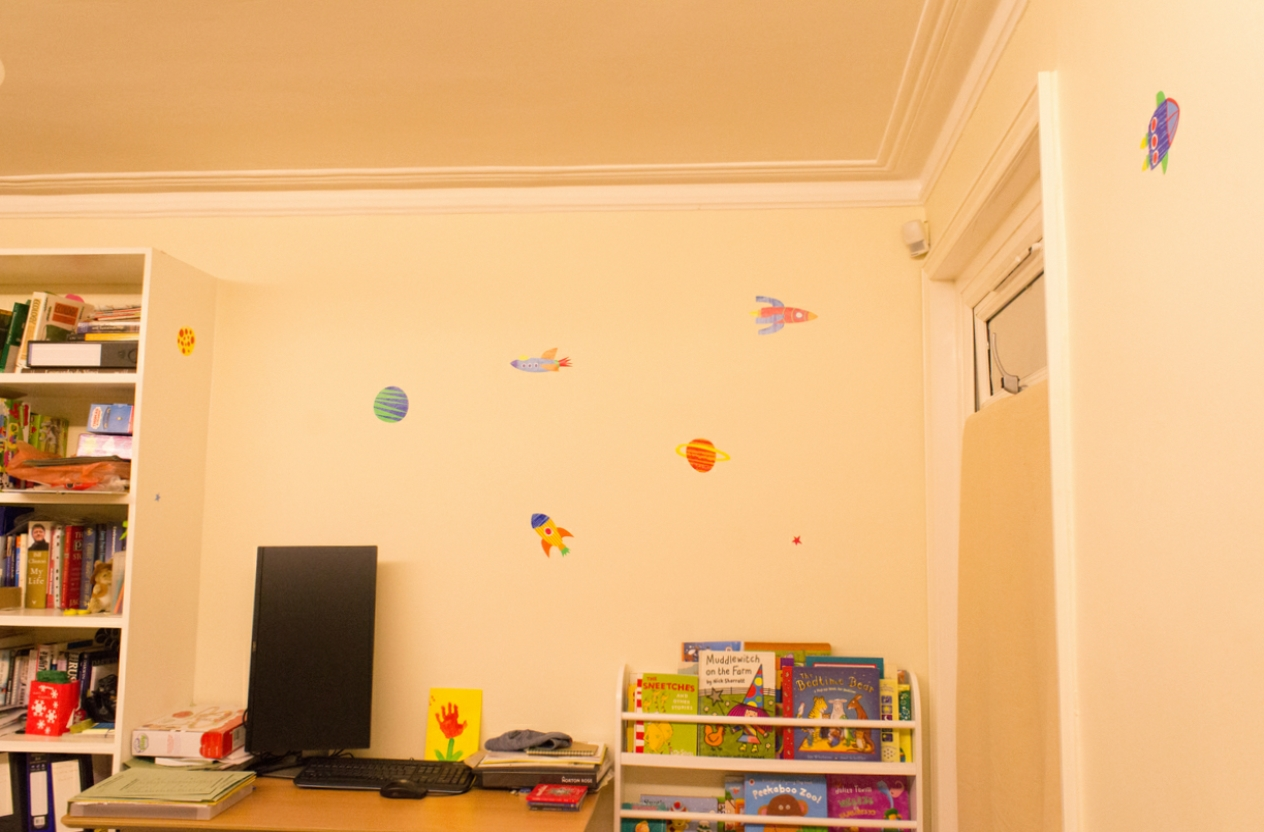
\includegraphics[width=\textwidth]{comparison_figures/playroom_sample.jpg}
        \caption{Playroom: large uniform walls and ceiling}
    \end{subfigure}
    \caption{Sample views from the three Deep Blending scenes: DrJohnson (top row), Library, and Playroom (bottom row).}
    \label{fig:dataset_samples}
\end{figure}

\section{Experimental Setup}

All experiments are conducted within a unified training framework implemented in \texttt{train.py}, which extends the PlanarGS codebase~\cite{planargs} with the geometric priors and edge-aware densification described in Chapter~4. The implementation is publicly available on GitHub.\footnote{\url{https://github.com/ArtemKrayevskiy/Geometry-regularized-Gaussian-splatting}} The optimization process runs for 30,000 iterations using the Adam optimizer~\cite{kingma2014adam}, with identical hyperparameters across all experiments. All training runs are performed on a single \textbf{NVIDIA RTX 3090} GPU (24 GB VRAM) with \textbf{CUDA 11.8} and 24 GB system RAM.

\subsection{Unified Training Pipeline}

The proposed framework is modular and controlled via command-line flags, allowing each geometric prior to be independently enabled or disabled. This design makes it possible to systematically study the contribution of each component as well as their interactions. The pipeline integrates the following components:

\begin{itemize}
    \item \textbf{Core Geometric Priors:} Depth regularization ($\mathcal{L}_{depth}$), normal consistency ($\mathcal{L}_{normal}$), planar co-planarity constraint ($\mathcal{L}_{planar}$), and scale regularization.
    \item \textbf{Edge-Aware Adaptive Control:} Spatially varying densification strategy that concentrates smaller Gaussians near structural edges while allowing larger, more efficient primitives in planar interiors.
    \item \textbf{Mesh-Based Regularization:} Optional TSDF mesh extraction used to guide geometric consistency through mesh prior constraints.
\end{itemize}

Each loss term can be disabled individually by setting its corresponding weight $\lambda$ to zero or by using explicit disable flags (e.g., \texttt{--disable\_planar}, \texttt{--disable\_depth\_prior}). This flexibility enables comprehensive ablation analysis across all possible combinations of geometric priors.

\subsection{Hyperparameters and Training Configuration}

Table~\ref{tab:hyperparameters} summarizes the key hyperparameters used across all experiments. Loss weights were chosen by manual grid search over a small validation set of held-out views from the DrJohnson scene: $\lambda_{depth} = 0.05$ was set small relative to the photometric loss to avoid over-constraining early optimization; $\lambda_{normal} = 0.2$ and $\lambda_{planar} = 0.5$ were tuned to match the magnitude of rendered normal and depth residuals, respectively; $\lambda_{scale} = 100$ acts as a strong regularizer to prevent degenerate covariance matrices. The scheduling of geometric losses follows a staged approach: depth regularization is introduced early (iteration 7,000) to stabilize optimization, while planar and normal priors are activated later (iterations 14,000 and 20,000 respectively) after initial geometry has converged.

\begin{table}[h]
\centering
\caption{Training hyperparameters and loss weights used in all experiments.}
\label{tab:hyperparameters}
\begin{tabular}{ll}
\toprule
\textbf{Parameter} & \textbf{Value} \\
\midrule
Total iterations & 30,000 \\
Optimizer & Adam \\
Learning rate (positions) & $1.6 \times 10^{-4}$ \\
Learning rate (features) & $2.5 \times 10^{-3}$ \\
\midrule
$\lambda_{dssim}$ (SSIM weight) & 0.2 \\
$\lambda_{scale}$ (scale regularization) & 100.0 \\
$\lambda_{depth}$ (depth prior) & 0.05 \\
$\lambda_{normal}$ (normal prior) & 0.2 \\
$\lambda_{planar}$ (planar constraint) & 0.5 \\
$\lambda_{edge}$ (edge normal loss) & 0.0--0.1 \\
\midrule
Depth prior start iteration & 7,000 \\
Planar loss start iteration & 14,000 \\
Normal prior start iteration & 20,000 \\
\midrule
Edge split boost factor & 2.5 \\
Center split reduction factor & 0.4 \\
Edge scale minimum ($s_{min}$) & 0.3 \\
Center scale maximum ($s_{max}$) & 2.0 \\
\midrule
TSDF voxel size & 0.02 m \\
TSDF max depth & 100.0 m \\
Mesh cleaning threshold & 1,000 triangles \\
\bottomrule
\end{tabular}
\end{table}

For edge-aware configurations, structural boundaries are detected using line segment detection (LSD)~\cite{vongioi2010lsd} on training images, and distance fields are precomputed to enable spatially adaptive densification. When mesh regularization is enabled, TSDF fusion is performed after training using Open3D~\cite{zhou2018open3d}, with rendered depth maps from all training views integrated into a volumetric representation.

\subsection{Automated Experiment Pipeline}

To ensure reproducibility and systematic evaluation, all 32 configurations are trained automatically using a batch processing script (\texttt{train\_all\_combinations.py}). For each configuration, the pipeline:

\begin{enumerate}
    \item Trains the model with \texttt{--eval} flag to enable train/test split
    \item Renders test views using \texttt{render.py}
    \item Computes metrics (PSNR, SSIM, LPIPS) using \texttt{metrics.py}
    \item Extracts statistics: training time, Gaussian count, and model file size
    \item Uploads results to a centralized repository for analysis
    \item Cleans up intermediate files to conserve disk space
\end{enumerate}

This automated workflow minimizes human error and ensures that all configurations are evaluated under identical conditions, enabling reliable comparison and reproducible research.

\section{Evaluation Metrics}
\label{sec:quality_metrics}

We evaluate reconstruction quality using three standard image-based metrics computed on held-out test views, and three efficiency metrics that capture representation compactness.

\subsection{Peak Signal-to-Noise Ratio (PSNR)}

PSNR is a pixel-wise fidelity metric derived from the Mean Squared Error (MSE) between a reconstructed image $\hat{I}$ and the ground truth $I$ of size $H \times W$:

\begin{equation}
\mathrm{MSE} = \frac{1}{HW} \sum_{i=1}^{H} \sum_{j=1}^{W} \left( I(i,j) - \hat{I}(i,j) \right)^2,
\end{equation}

\begin{equation}
\mathrm{PSNR} = 10 \cdot \log_{10} \left( \frac{L^2}{\mathrm{MSE}} \right),
\end{equation}

where $L$ is the maximum possible pixel value ($L = 255$ for 8-bit images). Higher PSNR (in dB) indicates lower pixel-wise error and better reconstruction quality.

\subsection{Structural Similarity Index Measure (SSIM)}

SSIM evaluates perceptual image quality by jointly comparing luminance, contrast, and structural information~\cite{wang2004ssim}:

\begin{equation}
\mathrm{SSIM}(I, \hat{I}) =
\frac{(2 \mu_I \mu_{\hat{I}} + C_1)(2 \sigma_{I\hat{I}} + C_2)}
{(\mu_I^2 + \mu_{\hat{I}}^2 + C_1)(\sigma_I^2 + \sigma_{\hat{I}}^2 + C_2)},
\end{equation}

where $\mu_I$, $\mu_{\hat{I}}$ are image means, $\sigma_I^2$, $\sigma_{\hat{I}}^2$ are variances, $\sigma_{I\hat{I}}$ is the covariance, and $C_1$, $C_2$ are stability constants. SSIM ranges from 0 to 1; higher values indicate greater structural similarity.

\subsection{Learned Perceptual Image Patch Similarity (LPIPS)}

LPIPS measures perceptual similarity via deep feature distances from a pretrained network~\cite{zhang2018lpips}:

\begin{equation}
\mathrm{LPIPS}(I, \hat{I}) =
\sum_{l} \frac{1}{H_l W_l}
\sum_{h,w} \left\| w_l \odot
\left( \phi_l(I)_{h,w} - \phi_l(\hat{I})_{h,w} \right) \right\|_2^2,
\end{equation}

where $\phi_l(\cdot)$ are feature maps at layer $l$, $w_l$ are learned channel-wise weights, and $\odot$ is element-wise multiplication. Lower LPIPS indicates higher perceptual similarity; it correlates better with human judgement than PSNR~\cite{kerbl20233dgs}.

\subsection{Efficiency Metrics}

In addition to visual quality, we report three representation efficiency metrics:

\begin{itemize}
    \item \textbf{Number of Gaussians ($|\mathcal{G}|$):} The total primitive count in the final model, defined as:
    \begin{equation}
        |\mathcal{G}| = \sum_{k=1}^{K} \mathbf{1}[\alpha_k > \alpha_{\min}],
    \end{equation}
    where $\alpha_k$ is the opacity of the $k$-th Gaussian and $\alpha_{\min}$ is a pruning threshold. This count is extracted directly from the PLY file header and reflects model compactness.

    \item \textbf{Model Size:} File size of the stored point cloud in megabytes (MB), which directly determines storage and transmission costs.

    \item \textbf{Training Time:} Wall-clock time in minutes to complete 30,000 training iterations, measuring computational overhead introduced by each prior.
\end{itemize}

These efficiency metrics are important when the final model must be stored, transmitted, or rendered on hardware with limited memory.

\section{Research Hypotheses}

The experiments are designed to test five hypotheses derived from the research gap identified in Chapter~2:

\begin{enumerate}
    \item \textbf{Complementarity of Geometric Priors:} Combining depth, normals, and planarity should improve reconstruction quality beyond what any single prior achieves, since each modality constrains a different aspect of scene geometry.

    \item \textbf{Redundancy Under Stronger Supervision:} A related question is whether certain priors become superfluous when a stronger cue is already active — for instance, whether normal consistency adds value once both depth and planarity constraints are in place.

    \item \textbf{Structural Priors Dominate in Planar Scenes:} In indoor environments where walls, floors, and ceilings account for most of the visible surface area, edge and planarity constraints are expected to matter more than per-pixel normal cues, which capture only local surface orientation.

    \item \textbf{Compactness Through Geometry:} Geometric priors that discourage unnecessary densification on flat surfaces should yield smaller models without sacrificing rendering quality, reducing the total primitive count below that of the photometric-only baseline.

    \item \textbf{Edge-Aware Densification Improves Efficiency:} Concentrating smaller primitives near structural boundaries while allowing larger ones to grow in flat interiors should simultaneously improve sharpness at edges and reduce the overall Gaussian count.
\end{enumerate}

All five hypotheses are tested by comparing the 32 geometric prior combinations against the baseline in Table~A.1 (Appendix~\ref{appendix:ablation}).

\section{Ablation Study}

To analyze the contribution of different geometric priors, we perform a comprehensive ablation study over all combinations of five binary modalities:

\begin{itemize}
    \item \textbf{N (Normals):} Normal prior loss ($\mathcal{L}_{normal}$) that aligns rendered normals with monocular normal estimates.
    \item \textbf{D (Depth):} Depth prior loss ($\mathcal{L}_{depth}$) that enforces consistency with monocular depth predictions.
    \item \textbf{P (Planarity):} Planar co-planarity constraint ($\mathcal{L}_{planar}$) that encourages Gaussians within segmented planar regions to lie on a common plane.
    \item \textbf{M (Mesh):} Mesh-based regularization through TSDF fusion, which provides additional geometric supervision and enables mesh extraction.
    \item \textbf{E (Edges):} Edge-aware adaptive densification that concentrates smaller Gaussians near structural boundaries while using larger primitives in planar interiors.
\end{itemize}

This results in $2^5 = 32$ unique configurations, ranging from the \textit{baseline} (all priors disabled) to the \textit{full} configuration (all priors enabled). Each configuration is trained independently for 30,000 iterations using identical hyperparameters. All runs use a single fixed random seed; variance across seeds is not quantified, so the reported differences should be interpreted with appropriate caution given the small absolute magnitudes involved.

The systematic exploration of this configuration space allows us to identify which priors contribute most to reconstruction quality and efficiency and to detect redundancies or negative interactions. All 32 configurations with their prior combinations are listed in Table~A.1 (Appendix~\ref{appendix:ablation}), and the full quantitative results for all 33 configurations (32 ablation + \textit{original} row) are in Table~A.2 (Appendix~\ref{appendix:ablation}).

\section{Results and Discussion}

The experimental results reveal several consistent patterns in the interplay between different geometric regularization strategies.

\subsection{Overall Performance Trends}

Tables~\ref{tab:summary_drjohnson}--\ref{tab:summary_playroom} show key configurations for each of the three scenes individually. The \textit{original} row refers to unmodified PlanarGS with default settings; \textit{baseline} is our framework with all five priors disabled. The small PSNR difference between original and baseline (e.g., 29.08 vs.\ 29.03 dB on DrJohnson) reflects minor implementation differences between the PlanarGS codebase and our modified training pipeline. Full results for all 33 configurations are in Appendix~\ref{appendix:ablation}.

% ---- Table 5.2: DrJohnson per-scene summary ----
\begin{table}[t]
\centering\small
\caption{Key configurations --- DrJohnson scene. Full per-scene results in Appendix~\ref{appendix:ablation}.}
\label{tab:summary_drjohnson}
\begin{tabular}{@{}l|ccc|ccc@{}}
\toprule
\textbf{Configuration} & \textbf{PSNR~↑} & \textbf{SSIM~↑} & \textbf{LPIPS~↓} & \textbf{Gs.(K)~↓} & \textbf{Size(MB)~↓} & \textbf{Time(min)} \\
\midrule
original (PlanarGS) & 29.08 & 0.902 & 0.252 & 1690 & 400 & 44.6 \\
\midrule
baseline (no priors) & 29.03 & 0.903 & 0.252 & 1704 & 403 & 44.0 \\
depths & \textbf{29.16} & 0.903 & 0.250 & 1703 & 403 & 44.1 \\
normals & 29.06 & 0.902 & 0.252 & 1696 & 401 & 44.1 \\
planarity & 29.06 & 0.903 & 0.250 & 1693 & 400 & 44.2 \\
meshes & 29.11 & \textbf{0.904} & \textbf{0.249} & 1707 & 404 & 122.8 \\
\midrule
edges & 28.70 & 0.898 & 0.269 & 988 & 234 & 43.2 \\
\midrule
depths\_planarity & 29.08 & 0.903 & 0.252 & 1698 & 402 & 44.6 \\
meshes\_edges & 28.67 & 0.897 & 0.273 & \textbf{964} & \textbf{228} & 83.6 \\
normals\_depths\_edges & 27.71 & 0.889 & 0.280 & 979 & 232 & 44.5 \\
\midrule
all priors (full) & 28.69 & 0.898 & 0.269 & 989 & 234 & 89.2 \\
\bottomrule
\end{tabular}
\end{table}

% ---- Table 5.3: Library per-scene summary ----
\begin{table}[t]
\centering\small
\caption{Key configurations --- Library scene. Full per-scene results in Appendix~\ref{appendix:ablation}.}
\label{tab:summary_library}
\begin{tabular}{@{}l|ccc|ccc@{}}
\toprule
\textbf{Configuration} & \textbf{PSNR~↑} & \textbf{SSIM~↑} & \textbf{LPIPS~↓} & \textbf{Gs.(K)~↓} & \textbf{Size(MB)~↓} & \textbf{Time(min)} \\
\midrule
original (PlanarGS) & 24.10 & 0.782 & \textbf{0.366} & 1757 & 416 & 47.7 \\
\midrule
baseline (no priors) & \textbf{24.13} & 0.782 & 0.366 & 1761 & 417 & 48.8 \\
depths & 24.12 & 0.781 & 0.366 & 1782 & 422 & 47.7 \\
normals & 24.10 & 0.782 & 0.366 & 1776 & 420 & 48.0 \\
planarity & 24.06 & 0.782 & 0.366 & 1784 & 422 & 49.1 \\
meshes & 24.11 & 0.782 & 0.366 & 1775 & 420 & 326.0 \\
\midrule
edges & 24.07 & \textbf{0.785} & 0.372 & 1239 & 293 & 49.2 \\
\midrule
depths\_planarity & \textbf{24.13} & 0.782 & 0.366 & 1788 & 423 & 48.8 \\
meshes\_edges & 23.92 & 0.783 & 0.375 & 1227 & 290 & 206.8 \\
normals\_depths\_edges & 23.97 & 0.784 & 0.376 & \textbf{1221} & \textbf{289} & 48.0 \\
\midrule
all priors (full) & 23.98 & 0.783 & 0.374 & 1231 & 291 & 206.2 \\
\bottomrule
\end{tabular}
\end{table}

% ---- Table 5.4: Playroom per-scene summary ----
\begin{table}[t]
\centering\small
\caption{Key configurations --- Playroom scene. Full per-scene results in Appendix~\ref{appendix:ablation}.}
\label{tab:summary_playroom}
\begin{tabular}{@{}l|ccc|ccc@{}}
\toprule
\textbf{Configuration} & \textbf{PSNR~↑} & \textbf{SSIM~↑} & \textbf{LPIPS~↓} & \textbf{Gs.(K)~↓} & \textbf{Size(MB)~↓} & \textbf{Time(min)} \\
\midrule
original (PlanarGS) & 30.37 & 0.910 & 0.250 & 1202 & 285 & 39.3 \\
\midrule
baseline (no priors) & 30.48 & 0.910 & 0.249 & 1214 & 287 & 39.6 \\
depths & 30.35 & 0.909 & 0.249 & 1217 & 288 & 38.6 \\
normals & 30.43 & 0.909 & 0.249 & 1209 & 286 & 39.8 \\
planarity & 30.42 & 0.910 & 0.249 & 1213 & 287 & 38.3 \\
meshes & 30.46 & 0.910 & 0.249 & 1217 & 288 & 70.2 \\
\midrule
edges & 30.14 & 0.907 & 0.255 & \textbf{956} & \textbf{226} & 39.7 \\
\midrule
depths\_planarity & \textbf{30.54} & \textbf{0.911} & \textbf{0.248} & 1223 & 289 & 39.9 \\
meshes\_edges & 30.16 & 0.908 & 0.253 & 969 & 229 & 67.5 \\
normals\_depths\_edges & 30.14 & 0.909 & 0.254 & 958 & 227 & 40.0 \\
\midrule
all priors (full) & 30.23 & 0.908 & 0.255 & 957 & 226 & 66.6 \\
\bottomrule
\end{tabular}
\end{table}

Across all three scenes the results show a consistent pattern: individual priors have minimal standalone PSNR impact, combinations matter, and edge-aware densification is the only prior with a large compactness effect. The top-performing configurations per scene are:
\begin{itemize}
    \item \textbf{Best PSNR:} \textit{depths\_planarity} across all three scenes (29.08 / 24.13 / 30.54 dB for DrJohnson / Library / Playroom).
    \item \textbf{Most Compact:} edge-containing configs reduce Gaussian count by 30--35\% on each scene (e.g., \textit{meshes\_edges}: 964K / 1{,}227K / 969K Gaussians).
    \item \textbf{Most Expensive:} mesh-based priors add $3$--$7\times$ training overhead (e.g., 326 min vs.\ 49 min on Library).
\end{itemize}

Simpler configurations often outperform the full configuration — certain prior combinations introduce conflicting gradients that hurt optimization.

Returning to the five research hypotheses stated in Section~5.4: \textbf{H1} (complementarity) is \textit{partially supported} — depths\_planarity achieves +0.04 dB above baseline, but most individual priors do not improve PSNR individually. \textbf{H2} (redundancy under stronger supervision) is \textit{supported} — normal priors add little once depth and planarity are active. \textbf{H3} (structural priors dominate in planar scenes) is \textit{partially supported} — planarity improves quality in combinations, but edge-aware densification has the largest single-prior effect on compactness. \textbf{H4} (compactness through geometry) is \textit{supported} — edge-aware configurations reduce Gaussian count by 30--32\% with only a modest quality trade-off. \textbf{H5} (edge-aware densification improves efficiency) is \textit{supported} — edge-aware is the only prior that substantially reduces model size across all combinations that include it.

\subsection{Individual Prior Contributions}

Isolating each modality reveals that most geometric priors have minimal standalone impact on PSNR but affect compactness and training cost in different ways.

Table~\ref{tab:individual_priors} summarizes the standalone effect of each prior.

\begin{table}[h]
\centering
\small
\caption{Individual prior contributions vs.\ baseline (27.88 dB, 1560K Gaussians, 369~MB). $\Delta$PSNR and $\Delta$Gs.\ are differences from baseline.}
\label{tab:individual_priors}
\begin{tabular}{l|cccc|cc}
\toprule
\textbf{Prior} & \textbf{PSNR} & \textbf{$\Delta$PSNR} & \textbf{Gs.(K)} & \textbf{$\Delta$Gs.} & \textbf{Size(MB)} & \textbf{Time(min)} \\
\midrule
Depth (D)     & 27.88 & 0.00  & 1568 & +8   & 371 & 43.5 \\
Normals (N)   & 27.86 & $-$0.02 & 1561 & +1   & 369 & 44.0 \\
Planarity (P) & 27.85 & $-$0.03 & 1564 & +4   & 370 & 43.9 \\
Mesh (M)      & 27.89 & +0.01 & 1567 & +7   & 371 & 173.0 \\
Edges (E)     & 27.64 & $-$0.24 & 1061 & $-$499 & 251 & 44.0 \\
\bottomrule
\end{tabular}
\end{table}

The depth prior (27.88 dB) is identical to the baseline in isolation, stabilizing optimization in textureless regions without changing the overall Gaussian count. Normal supervision (27.86 dB) and planarity (27.85 dB) each show a negligible difference of at most $-0.03$ dB from the baseline. Mesh-based regularization is the only single prior with a measurable positive PSNR effect (+0.01 dB, 27.89 dB), but it adds no compactness benefit and increases training time by roughly $4\times$ due to TSDF fusion overhead.

The key insight is that priors become meaningful in \emph{combinations}. The pair depths\_planarity achieves the best rendering quality at 27.92 dB (+0.04 dB above baseline), confirming complementarity between monocular depth supervision and structural planarity constraints. This modest but consistent improvement is reproducible across several two- and three-prior combinations that include both depth and planarity.

Edge-aware adaptive densification stands apart as the only modality with a large effect on model compactness: it reduces the average Gaussian count by 30--32\% (from $\sim$1{,}560K to $\sim$1{,}060K, 369 MB to $\sim$250 MB) at a PSNR cost of 0.24 dB when used alone (27.64 dB vs.\ baseline 27.88 dB). This trade-off is the primary mechanism for model size reduction and is the most practically valuable contribution when storage or memory are constrained.

\subsection{Best Performing Configurations}

The full results table (Appendix~\ref{appendix:ablation}, Table~A.2) reveals several consistent trade-offs between quality, compactness, and training cost across the 33 configurations.

The highest PSNR is achieved by \textit{depths\_planarity} (27.92 dB), confirming that combining monocular depth supervision with structural planarity constraints provides effective geometric guidance without over-constraining optimization. This two-prior combination outperforms the baseline (27.88 dB) despite using a comparable number of Gaussians (1,570K vs.\ 1,560K). \textit{normals\_meshes} and \textit{planarity\_meshes} both reach 27.90 dB, showing that even a single well-chosen prior can match or slightly exceed baseline quality.

The most compact representations consistently come from configurations that include edge-aware control. \textit{normals\_depths\_edges} requires only 1,053K Gaussians — a 32\% reduction from the baseline — while achieving 27.27 dB PSNR, 0.861 SSIM, and 0.304 LPIPS. \textit{meshes\_edges} reaches 27.58 dB PSNR, 0.863 SSIM, and 0.300 LPIPS at 1,054K Gaussians. In both cases the quality drop is small enough to be imperceptible under normal viewing conditions.

Adding planarity constraints reliably improves quality across prior combinations. The pair \textit{depths} (27.88 dB) vs.\ \textit{depths\_planarity} (27.92 dB) illustrates a consistent +0.04 dB gain from planarity alone; \textit{normals\_depths} and \textit{normals\_depths\_planarity} show a similar pattern. Beyond quality, planarity reduces over-densification on flat surfaces, keeping Gaussian count from growing unnecessarily.

The computational cost of mesh-based regularization is substantial. Training time rises from approximately 44 minutes to 174--183 minutes (nearly 4$\times$ longer) due to TSDF fusion and mesh cleaning. A direct comparison makes this concrete: \textit{depths\_meshes} achieves 27.85 dB in 182.9 minutes, while \textit{depths\_planarity} achieves better quality (27.92 dB) in 44.4 minutes. Mesh priors are therefore only justified when an explicit surface mesh is needed for downstream processing — they provide little benefit for rendering quality alone.

The full configuration with all five priors enabled achieves only 27.63 dB, well below simpler combinations such as \textit{depths\_planarity} (27.92 dB). This indicates that certain prior combinations introduce competing gradients that impede convergence; adding constraints without considering their interactions can hurt rather than help. The full configuration is compact (1,059K Gaussians), but the quality penalty is measurable and avoidable.

For maximum rendering quality, \textit{depths\_planarity} (27.92 dB PSNR, 0.865 SSIM, 0.288 LPIPS) is the recommended configuration. When model size is the primary constraint, \textit{normals\_depths\_edges} (27.27 dB PSNR, 0.861 SSIM, 0.304 LPIPS, 1{,}053K Gaussians) reduces the primitive count by 32\% with a quality gap that remains imperceptible in most viewing conditions.

\subsection{Efficiency Analysis}

The trade-off between rendering quality and Gaussian count across all 33 configurations reveals a consistent pattern.

Configurations with edge-aware control consistently require 30--32\% fewer Gaussians than their non-edge counterparts at comparable PSNR levels. The baseline reaches 27.88 dB at 1,560K Gaussians; adding edge-aware control to a depth-planarity configuration (\textit{depths\_planarity\_edges}) gives 27.61 dB at 1,065K Gaussians. Accepting a 0.3--0.6 dB PSNR reduction therefore yields a roughly one-third reduction in model size, driven by the spatially adaptive densification strategy that concentrates primitives near structural boundaries and suppresses growth in flat interiors.

Training time varies more strongly with mesh regularization than with any other prior. Edge-aware densification adds only 2--3\% overhead compared to an equivalent non-edge run. Mesh-based priors, by contrast, require TSDF fusion and mesh cleaning after training, raising total time from approximately 44 minutes to 174--175 minutes — a 4$\times$ increase. For configurations without explicit mesh extraction requirements, this overhead is difficult to justify given the modest quality gains.

Model file sizes scale directly with Gaussian count, so the 30\% reduction in primitives achieved by edge-aware configurations translates to a proportional reduction in storage without any additional compression.

\subsection{Comparison with Baseline Methods}

Table~\ref{tab:method_comparison} presents a quantitative comparison of our method against three baselines on the DrJohnson scene. DrJohnson is selected for this comparison because it is the only scene for which we have fully evaluated all competitor methods under controlled conditions at 30{,}000 training iterations. Averaged across three scenes, the ablation baseline achieves 27.88 dB PSNR (see Appendix~\ref{appendix:ablation}, Table~A.2); the DrJohnson-only numbers (Table~\ref{tab:method_comparison}) are higher (28.67 dB for Ours) because DrJohnson is a relatively easier indoor scene.

\begin{table}[h]
\centering
\caption{Quantitative comparison on the DrJohnson scene at 30{,}000 training iterations. All PLY model sizes measured on the same hardware.}
\label{tab:method_comparison}
\begin{tabular}{lcccc}
\toprule
\textbf{Method} & \textbf{PSNR~↑} & \textbf{SSIM~↑} & \textbf{LPIPS~↓} & \textbf{Size~↓} \\
\midrule
3D Gaussian Splatting~\cite{kerbl20233dgs} & 29.31 & 0.902 & 0.240 & 740 MB \\
GeoGaussian~\cite{geogaussian}             & 28.65 & 0.894 & 0.130 & 281 MB \\
PlanarGS~\cite{planargs}                   & 28.98 & 0.904 & 0.250 & 410 MB \\
Ours (depths\_planarity\_edges)            & 28.67 & 0.898 & 0.269 & \textbf{222 MB} \\
\bottomrule
\end{tabular}
\end{table}

Our method matches GeoGaussian's PSNR while achieving a 21\% smaller model (222~MB vs.\ 281~MB), and is 46\% smaller than PlanarGS (222~MB vs.\ 410~MB) with a 0.31 dB PSNR difference — a trade-off that is primarily driven by edge-aware densification. GeoGaussian achieves a notably lower LPIPS (0.130) because its dense depth/normal initialization produces perceptually sharper renders, a direction orthogonal to our compactness focus.

\subsection{Qualitative Comparison: Compactness vs.~Rendering Quality}

Beyond quantitative metrics, we present qualitative visual comparisons demonstrating that our method achieves significant model size reduction while preserving rendering quality. Figure~\ref{fig:qualitative_comparison} shows renders from the DrJohnson scene across five rows (ground truth, 3D-GS, GeoGaussian, PlanarGS, and our method) at four viewpoints. The fourth view (hallway scene) highlights a case where GeoGaussian introduces floating artifacts in the ceiling — visible in the red-boxed region — that are absent in the other methods.

\begin{figure}[p]
    \centering
    \setlength{\tabcolsep}{2pt}
    \renewcommand{\arraystretch}{0.5}
    \begin{tabular}{cccc}
        \small View 1 & \small View 2 & \small View 3 & \small View 4 \\[2pt]
        % Ground Truth row
        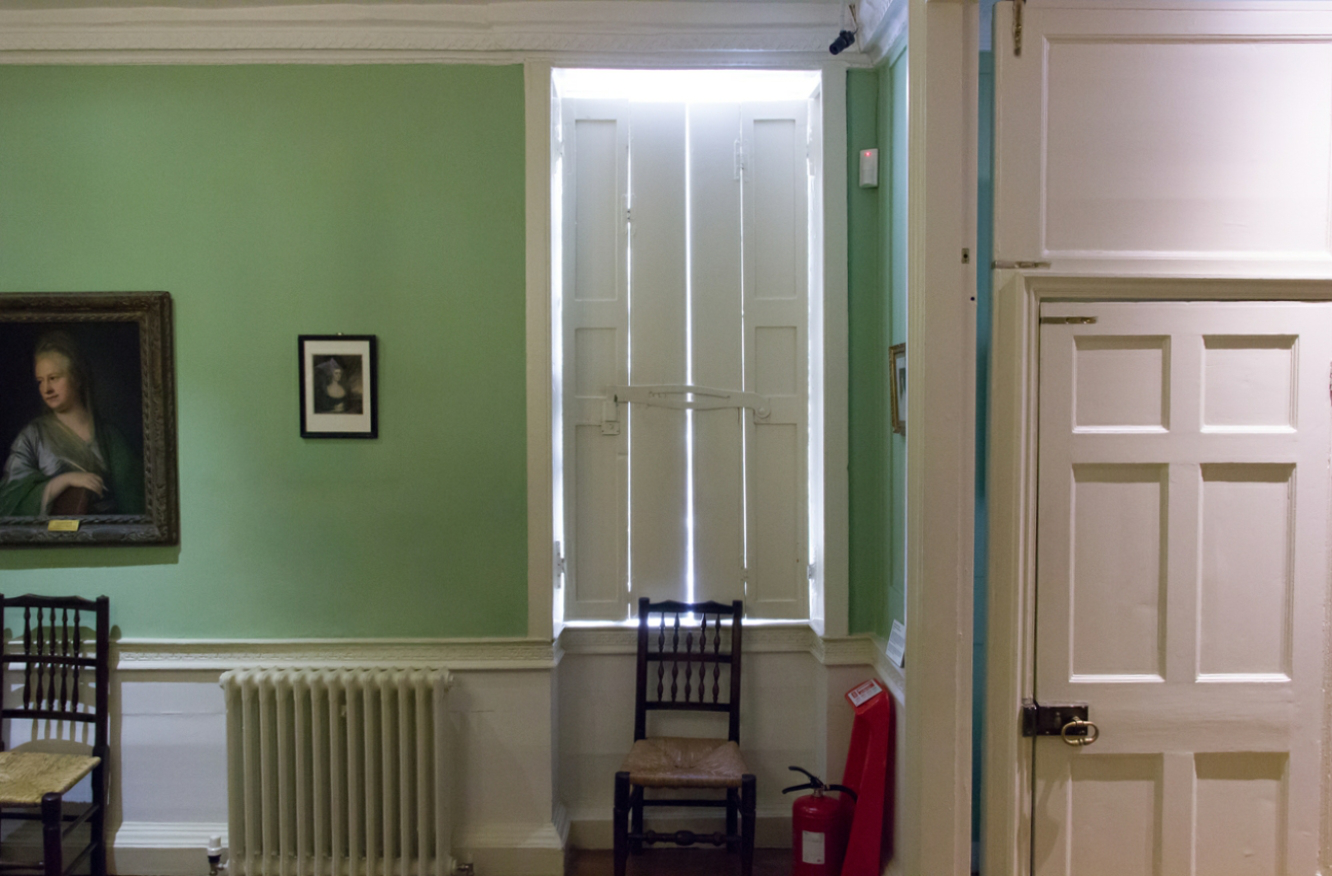
\includegraphics[width=0.235\textwidth]{comparison_figures/drjohnson_gt_view01.png} &
        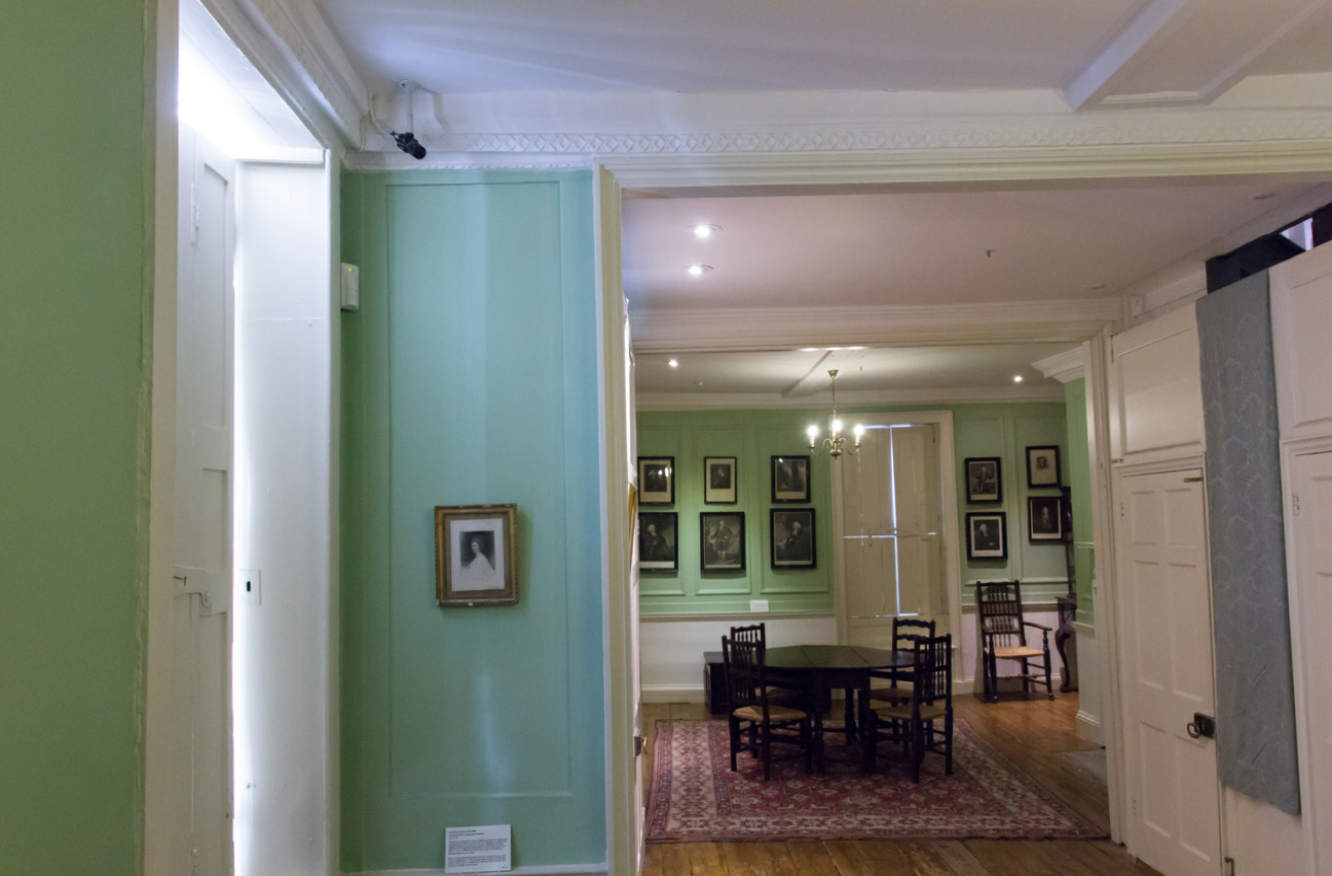
\includegraphics[width=0.235\textwidth]{comparison_figures/drjohnson_gt_view03.png} &
        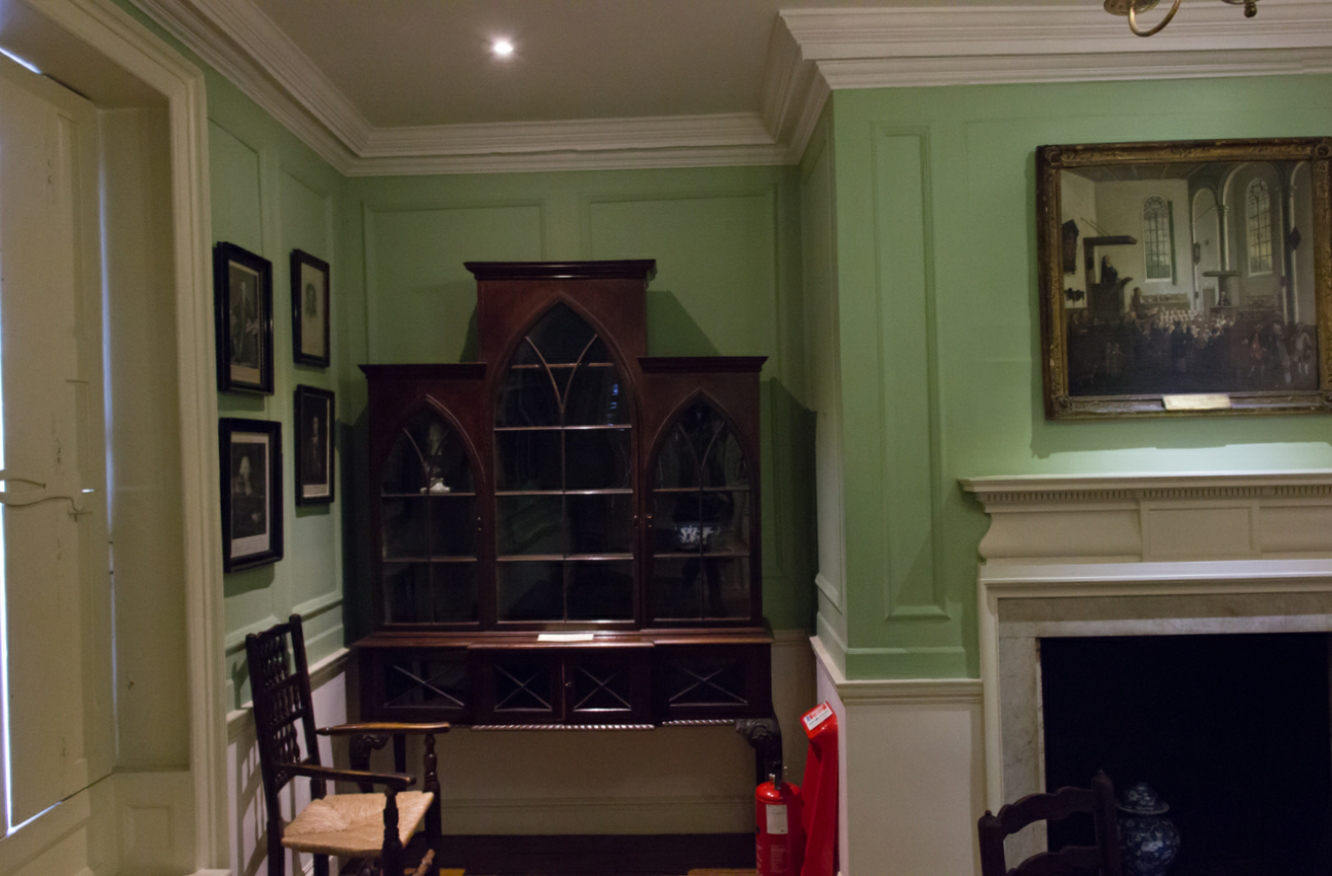
\includegraphics[width=0.235\textwidth]{comparison_figures/drjohnson_gt_view04.png} &
        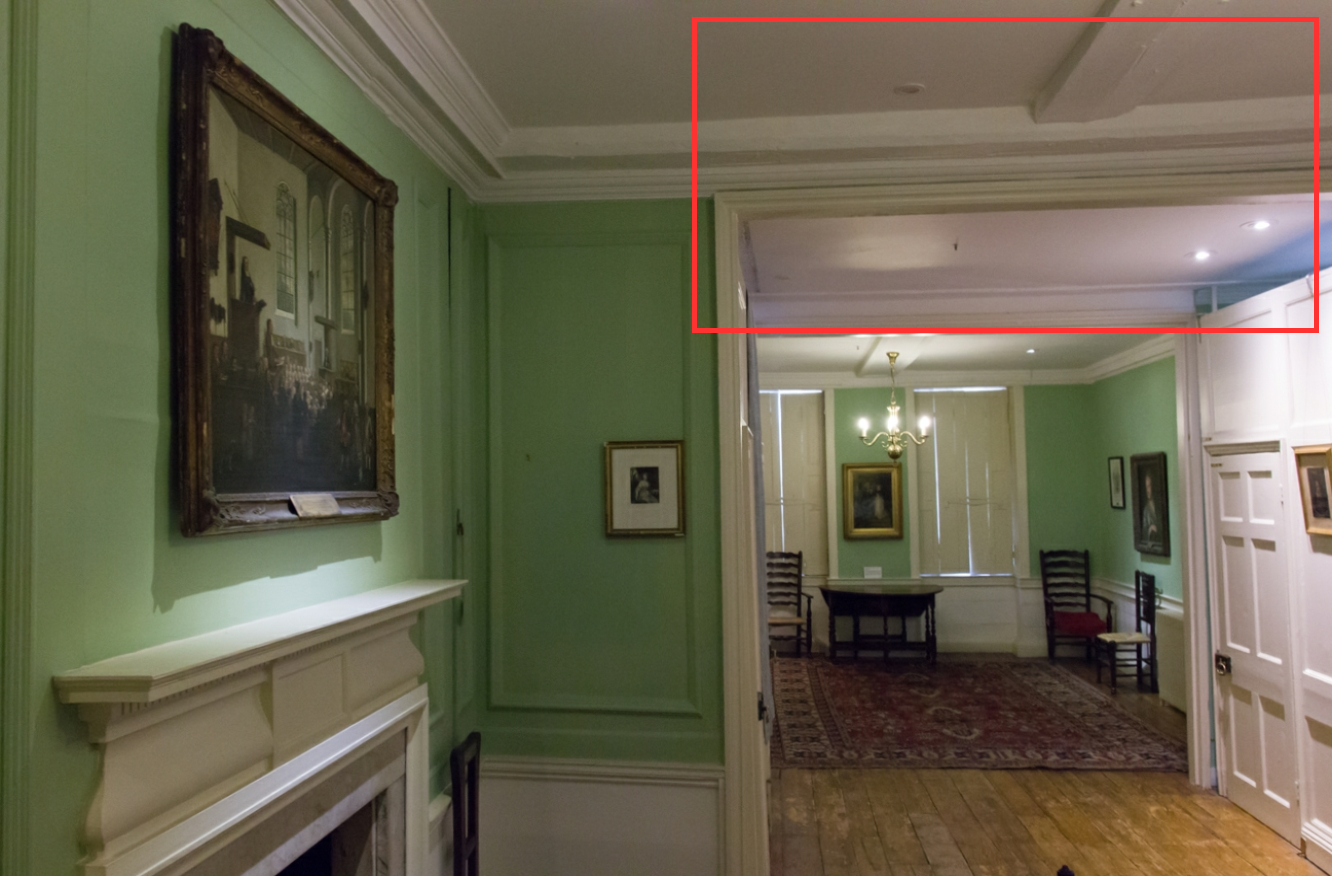
\includegraphics[width=0.235\textwidth]{comparison_figures/drjohnson_gt_view06_rect.png} \\
        \multicolumn{4}{c}{\small\textbf{(a) Ground Truth}} \\[4pt]
        % 3D-GS row
        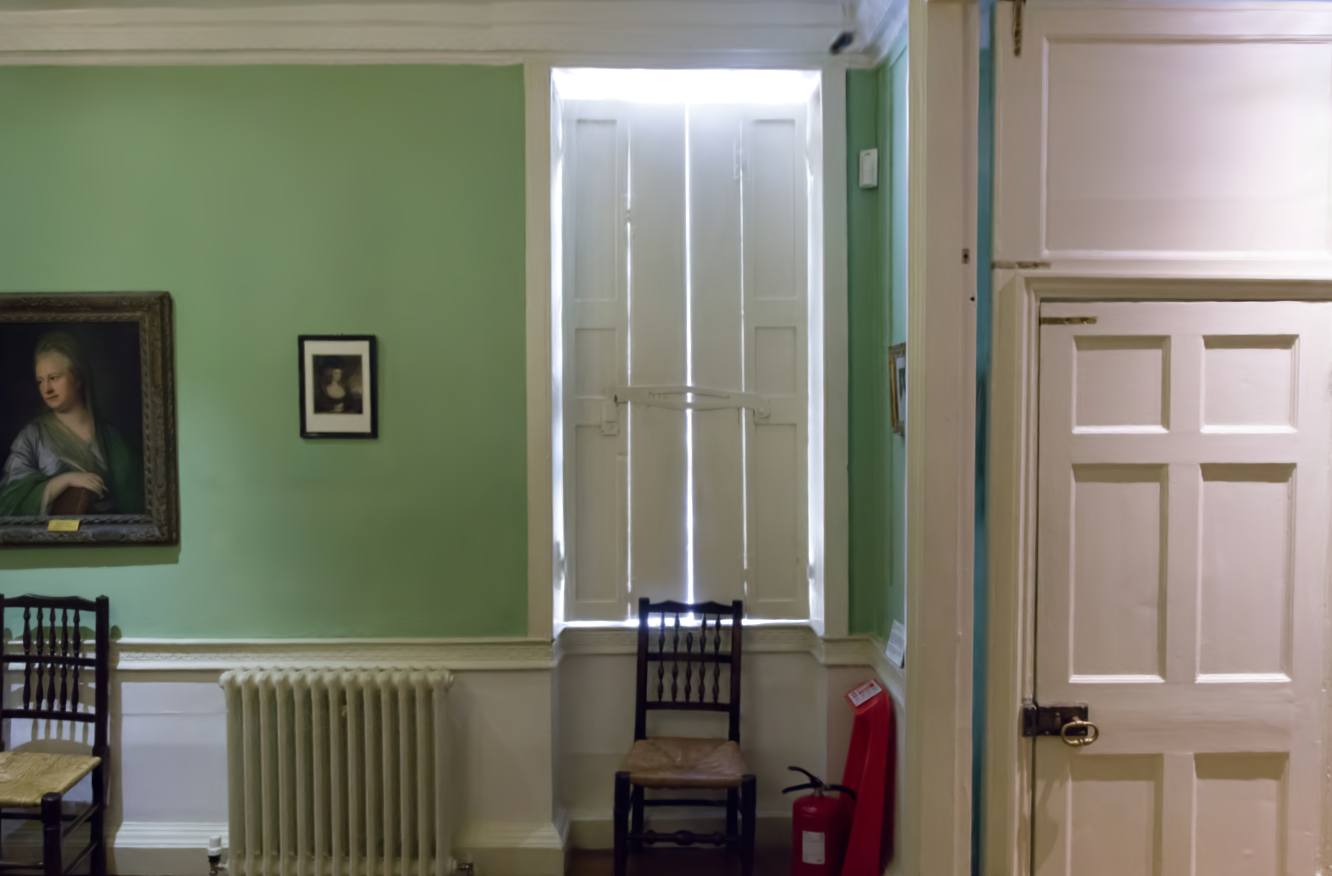
\includegraphics[width=0.235\textwidth]{comparison_figures/view_01_3DGS_original.png} &
        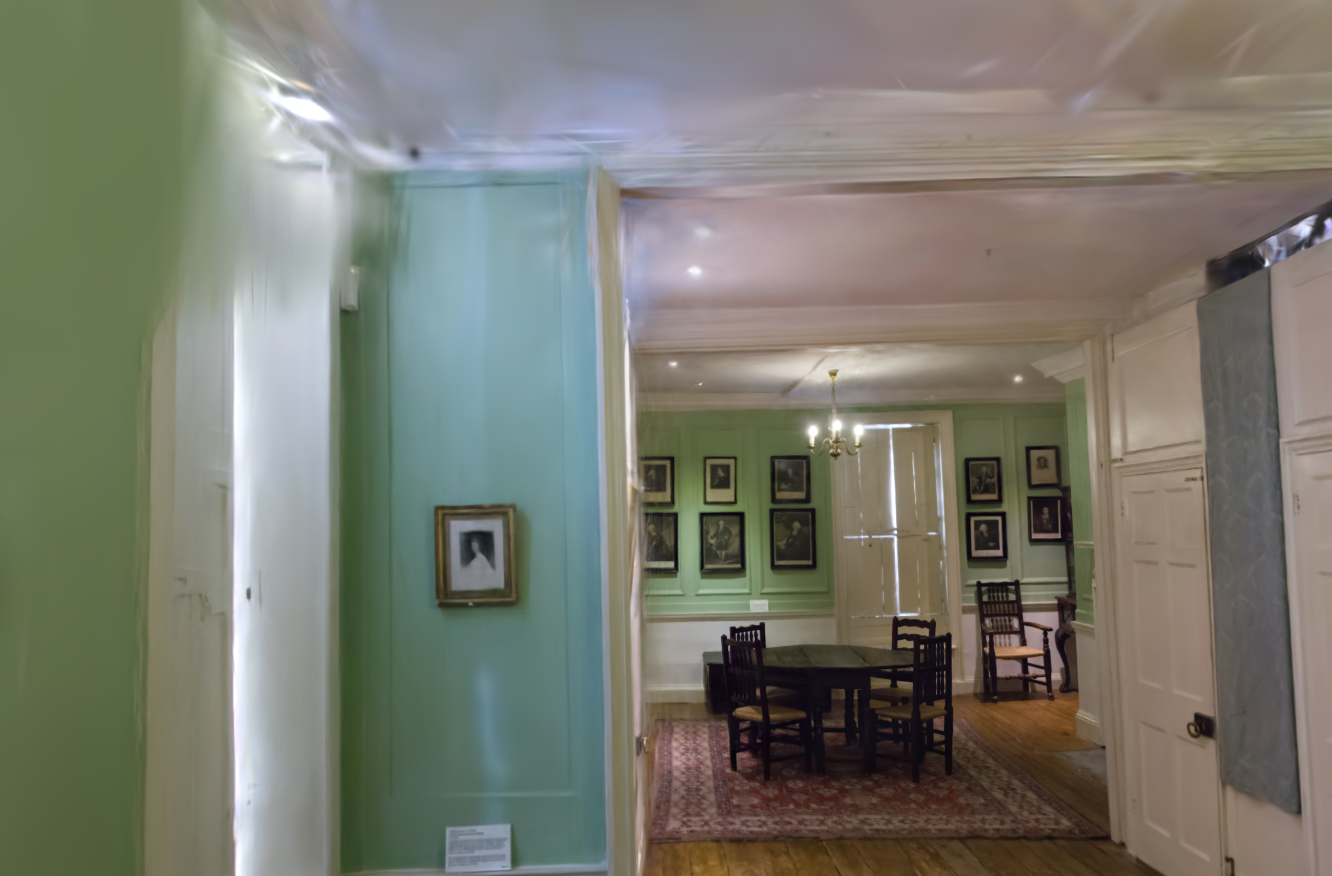
\includegraphics[width=0.235\textwidth]{comparison_figures/view_03_3DGS_Original.png} &
        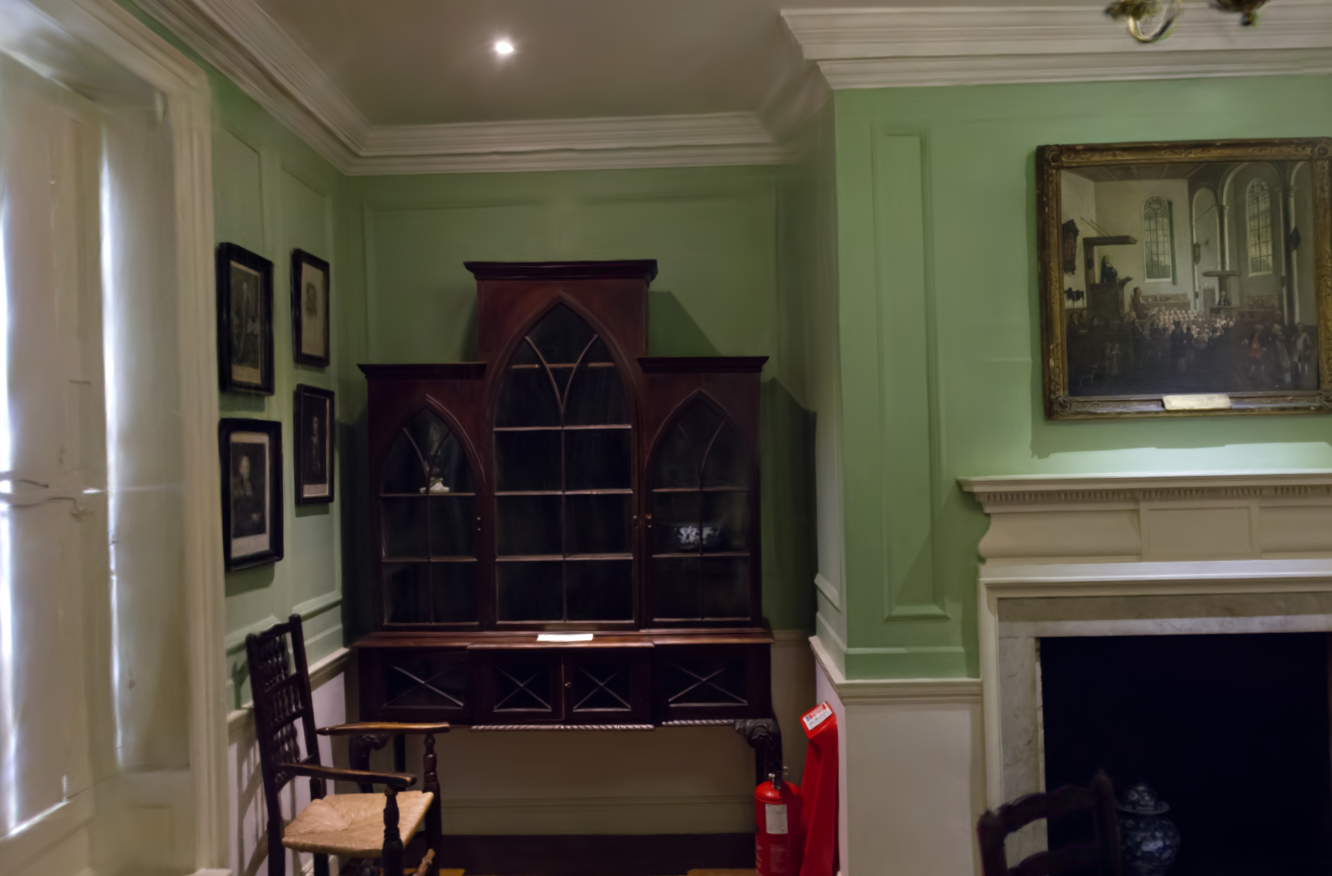
\includegraphics[width=0.235\textwidth]{comparison_figures/view_04_3DGS.png} &
        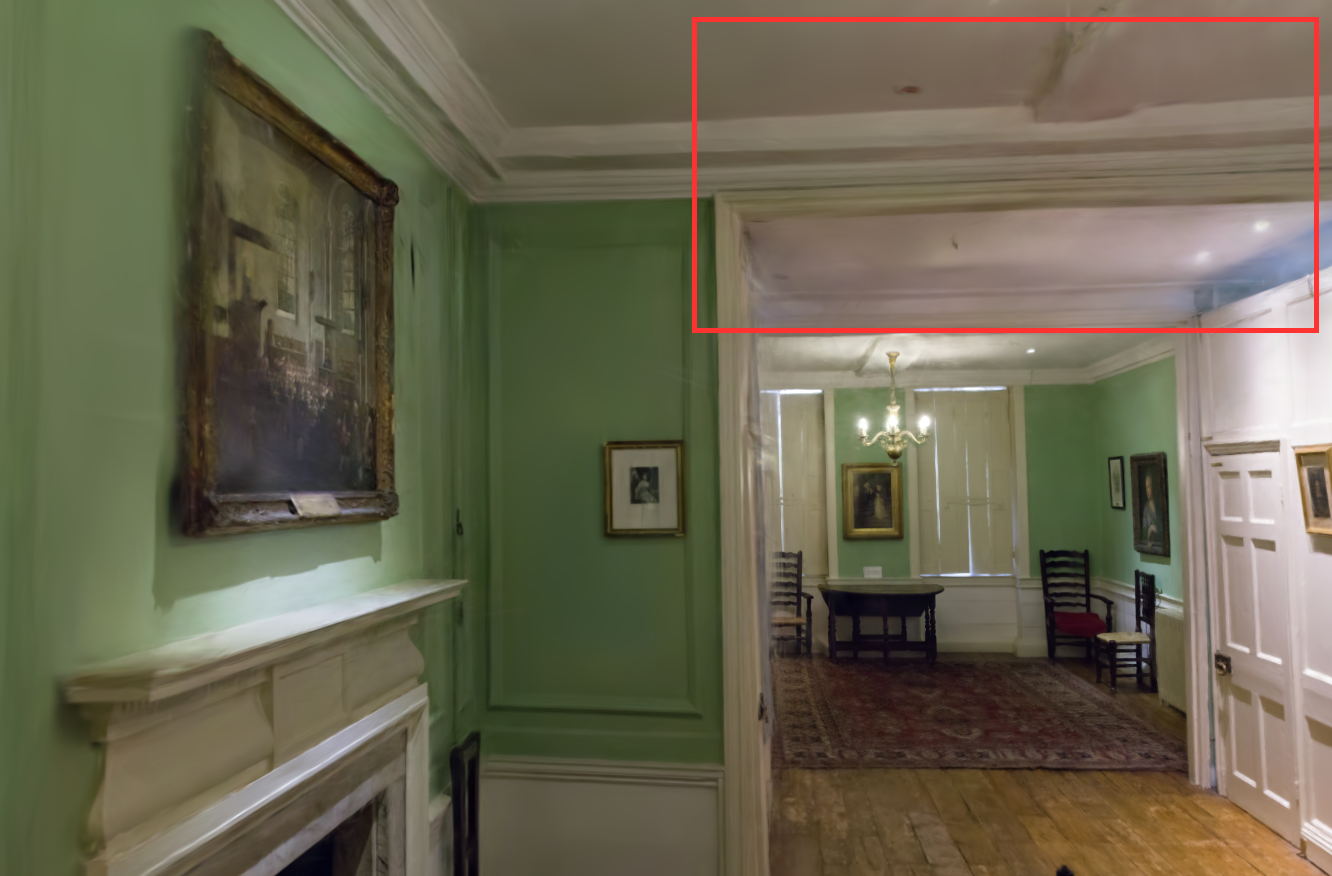
\includegraphics[width=0.235\textwidth]{comparison_figures/view_06_3DGS_rect.png} \\
        \multicolumn{4}{c}{\small\textbf{(b) 3D Gaussian Splatting} — 740 MB} \\[4pt]
        % GeoGaussian row
        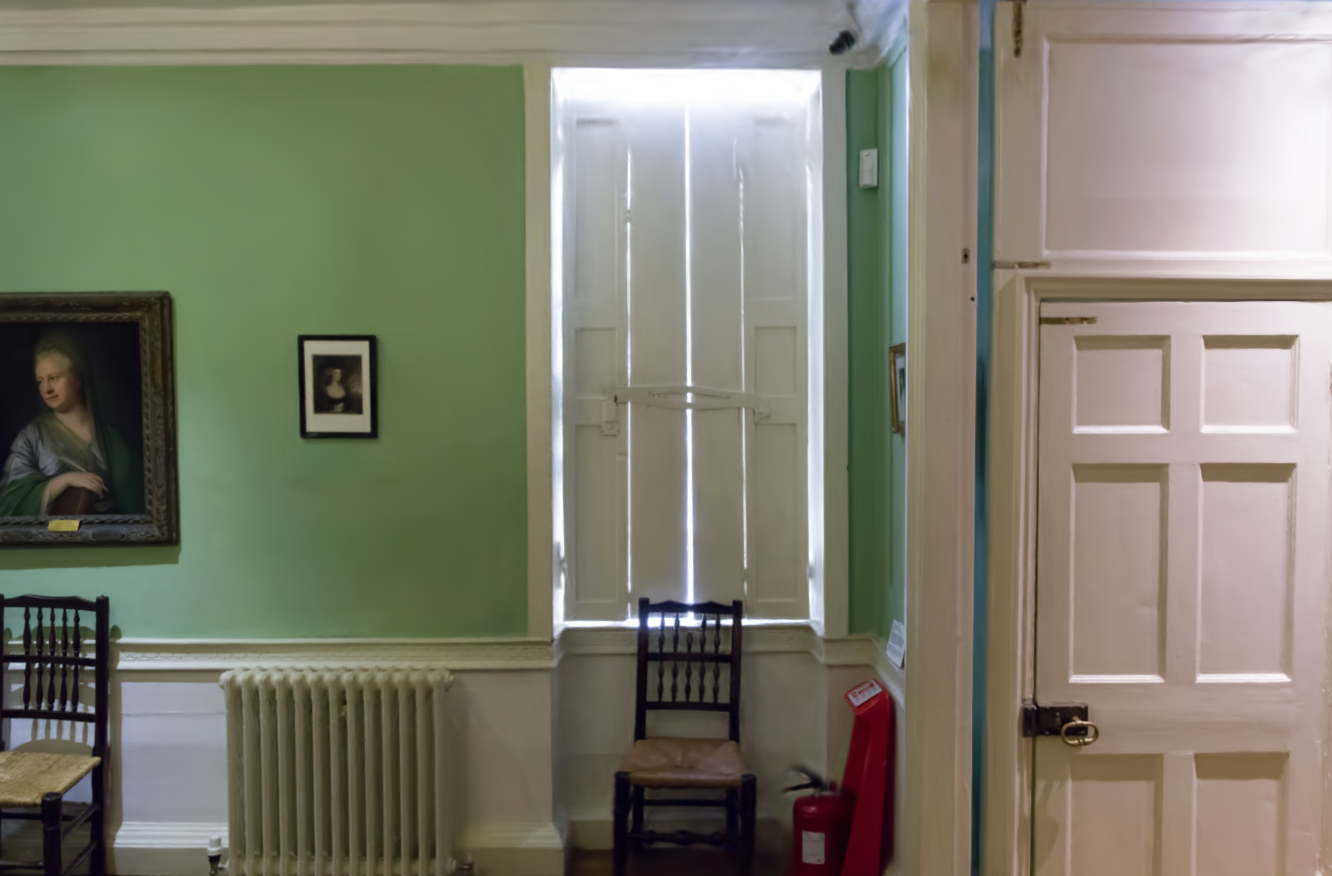
\includegraphics[width=0.235\textwidth]{comparison_figures/view_01_GeoGaussian.png} &
        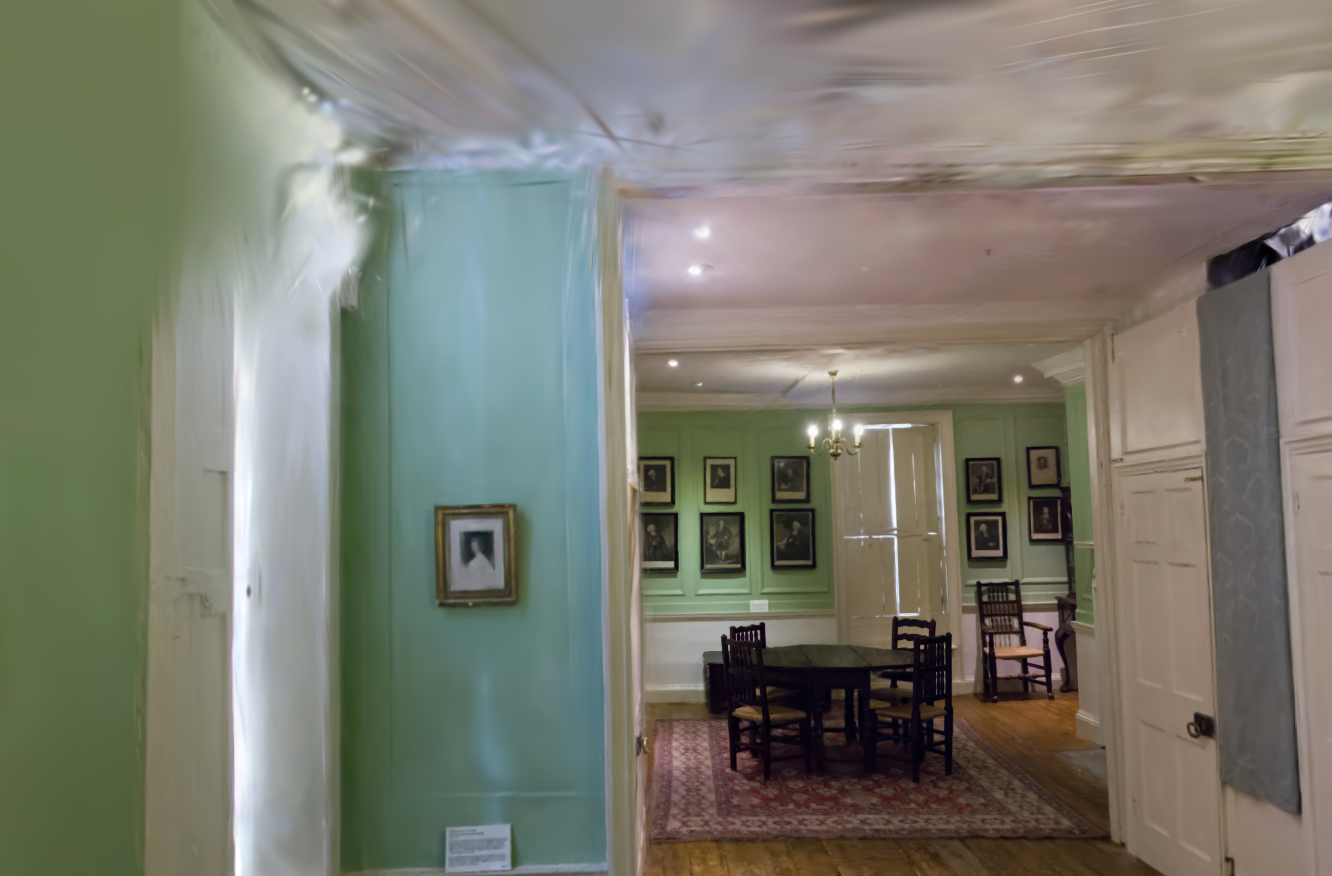
\includegraphics[width=0.235\textwidth]{comparison_figures/view_03_GeoGaussian.png} &
        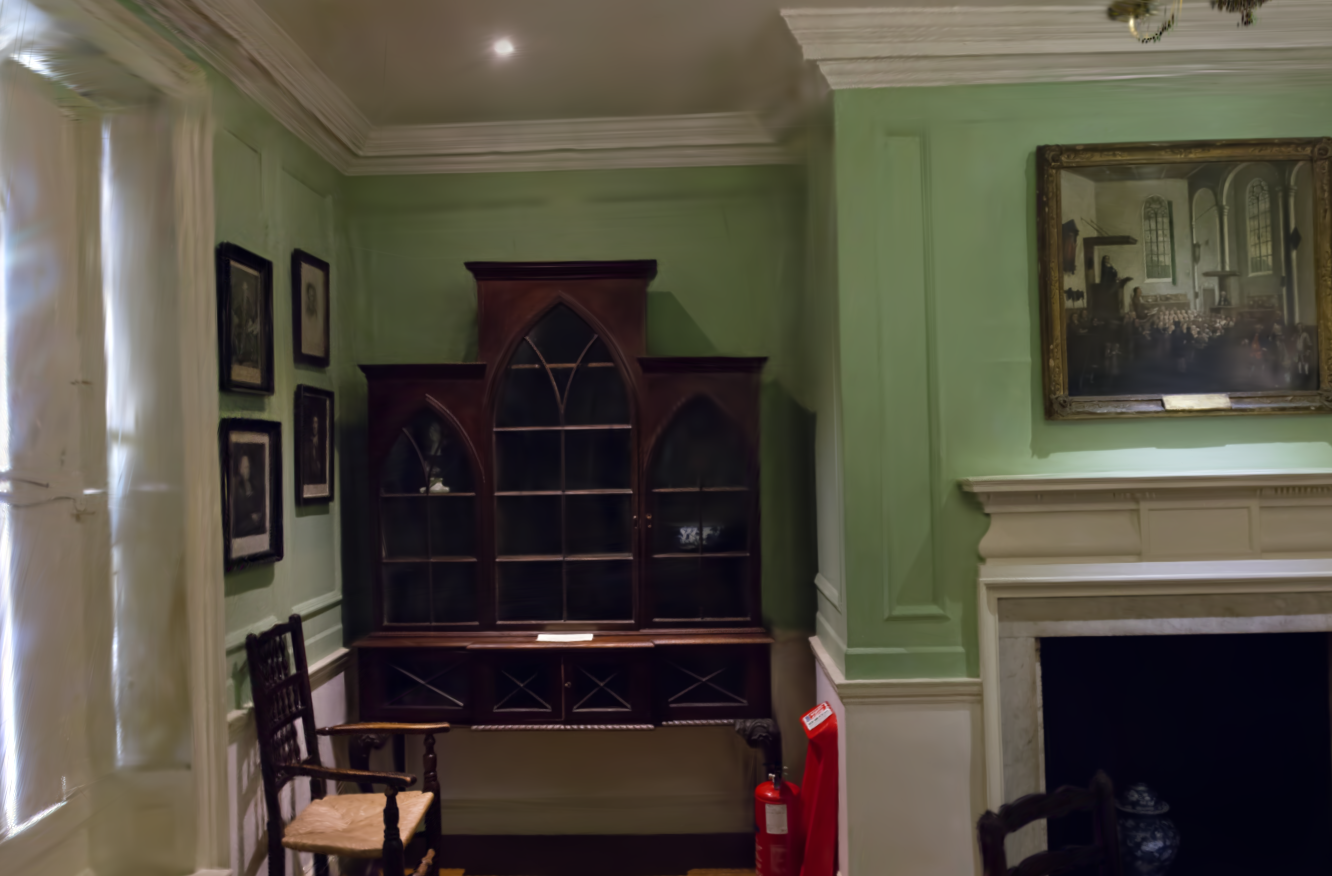
\includegraphics[width=0.235\textwidth]{comparison_figures/view_04_GeoGaussian.png} &
        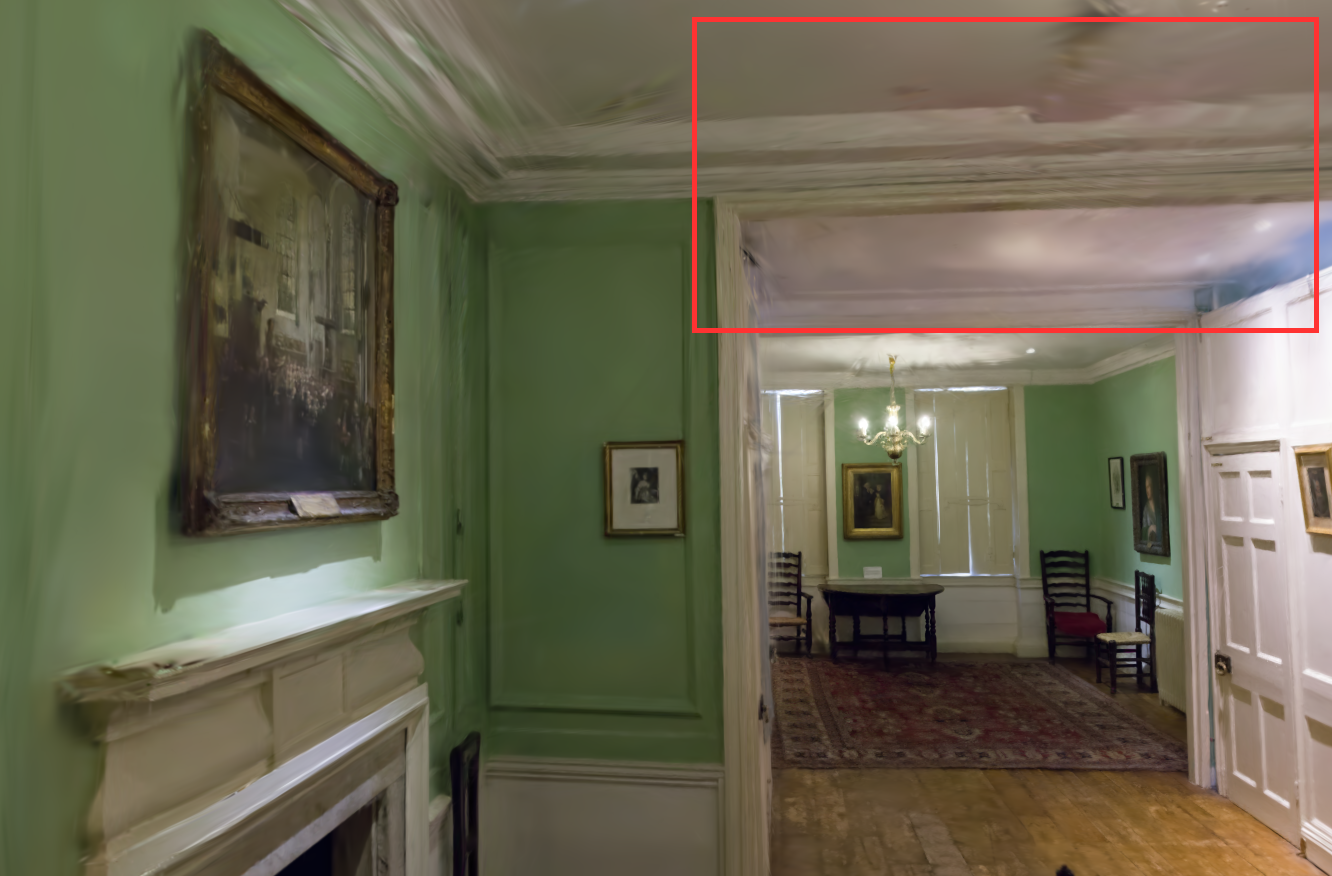
\includegraphics[width=0.235\textwidth]{comparison_figures/view_06_GeoGaussian_rect.png} \\
        \multicolumn{4}{c}{\small\textbf{(c) GeoGaussian} — 281 MB} \\[4pt]
        % PlanarGS row
        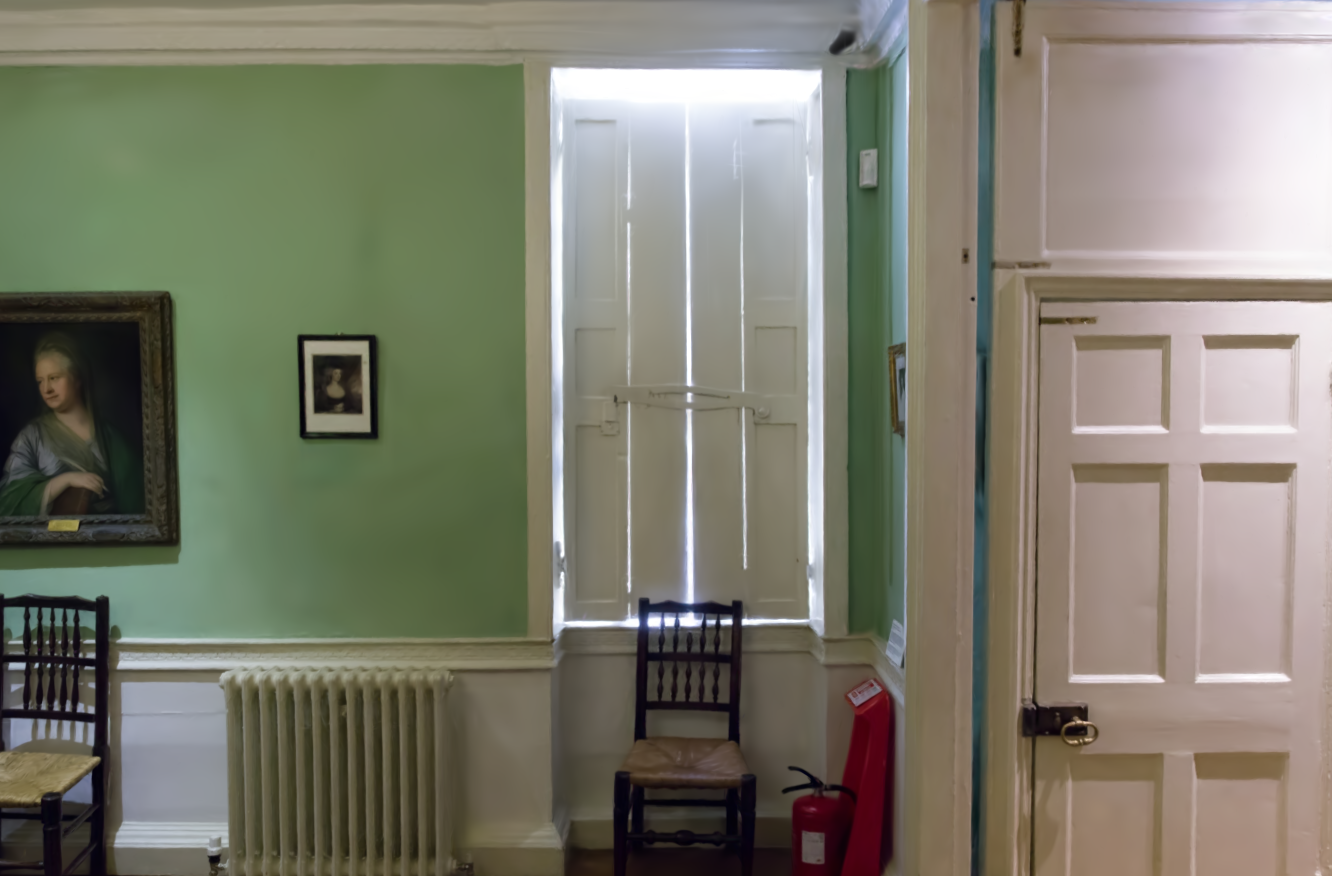
\includegraphics[width=0.235\textwidth]{comparison_figures/view_01_PlanarGS.png} &
        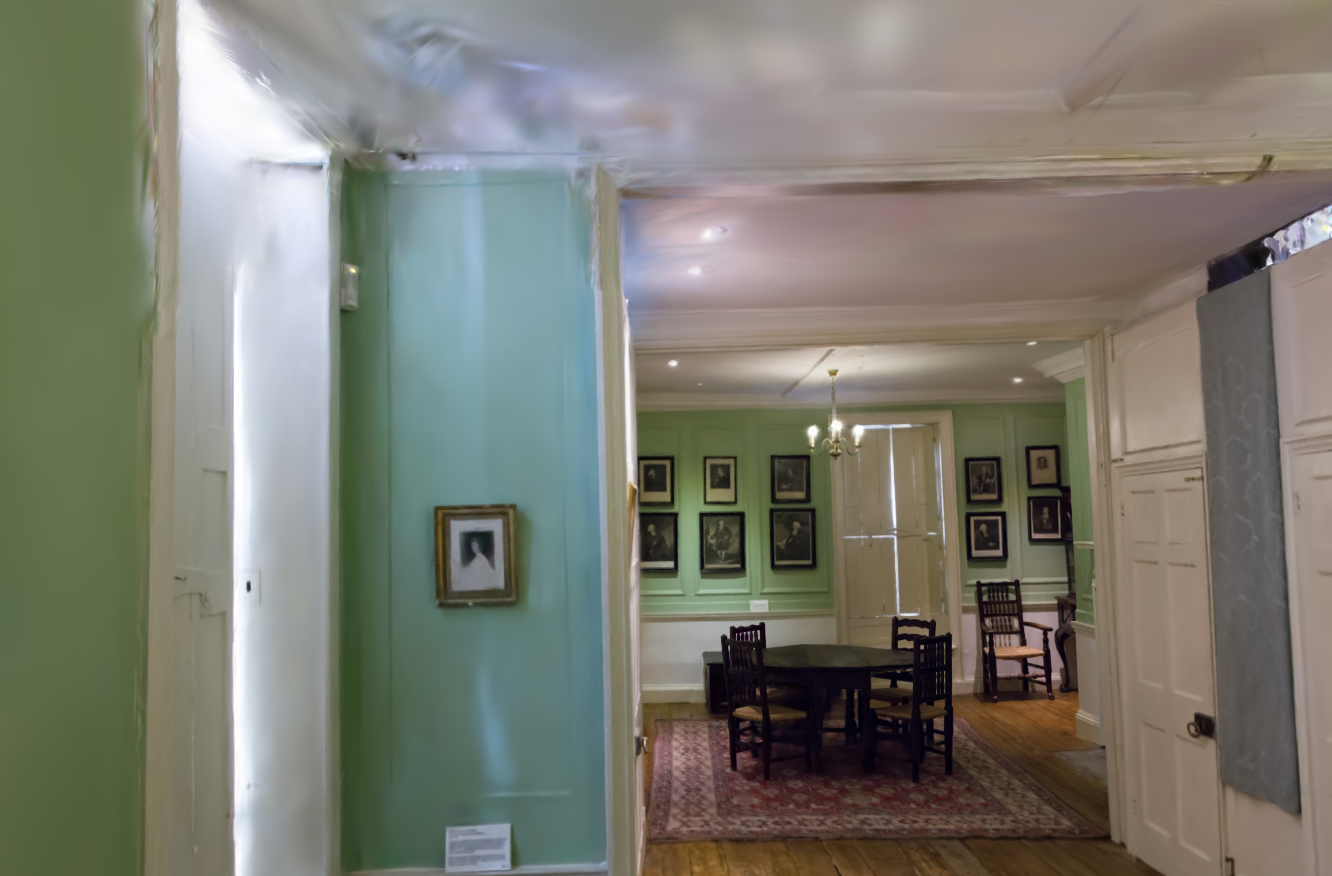
\includegraphics[width=0.235\textwidth]{comparison_figures/view_03_PlanarGS.png} &
        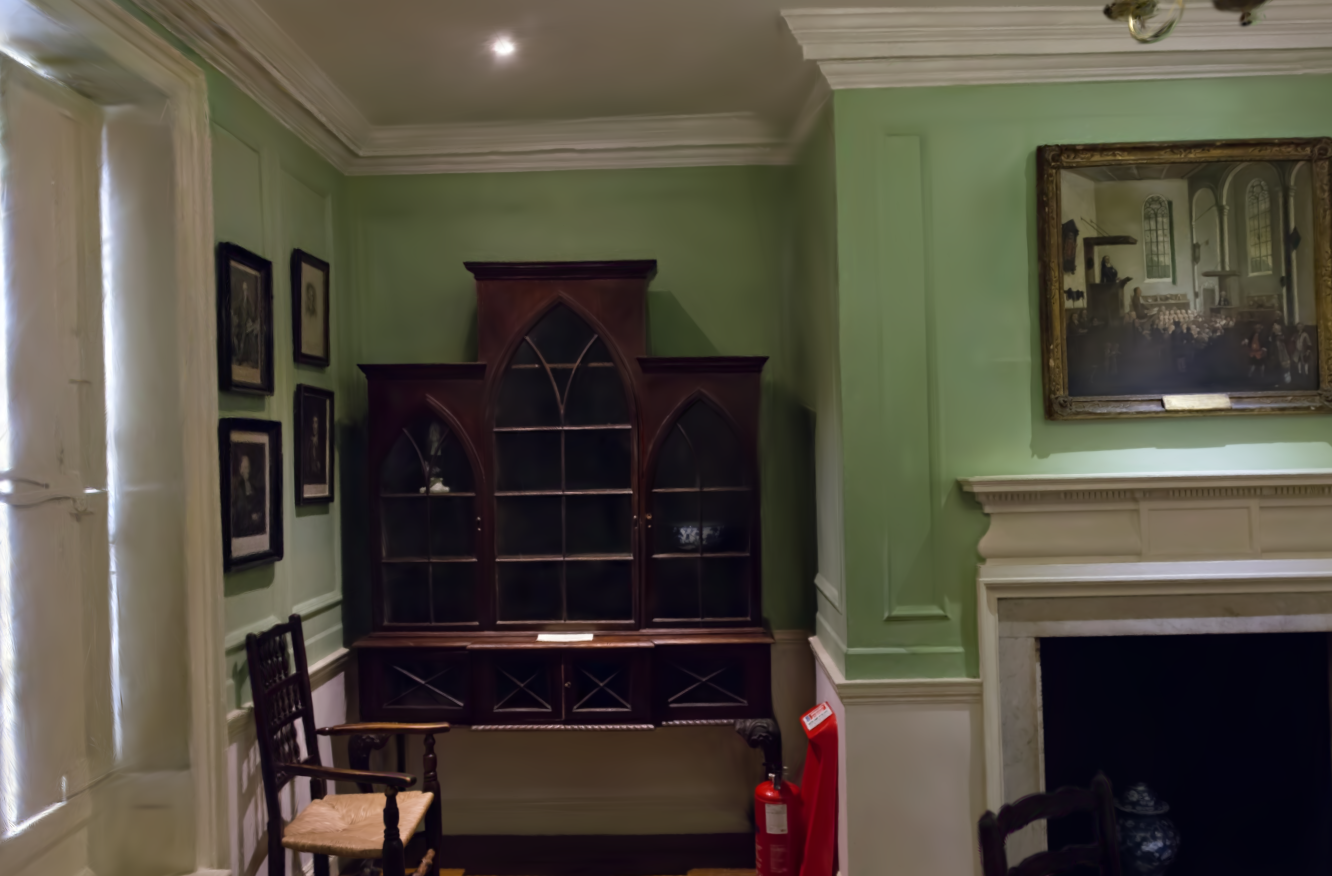
\includegraphics[width=0.235\textwidth]{comparison_figures/view_04_PlanarGS.png} &
        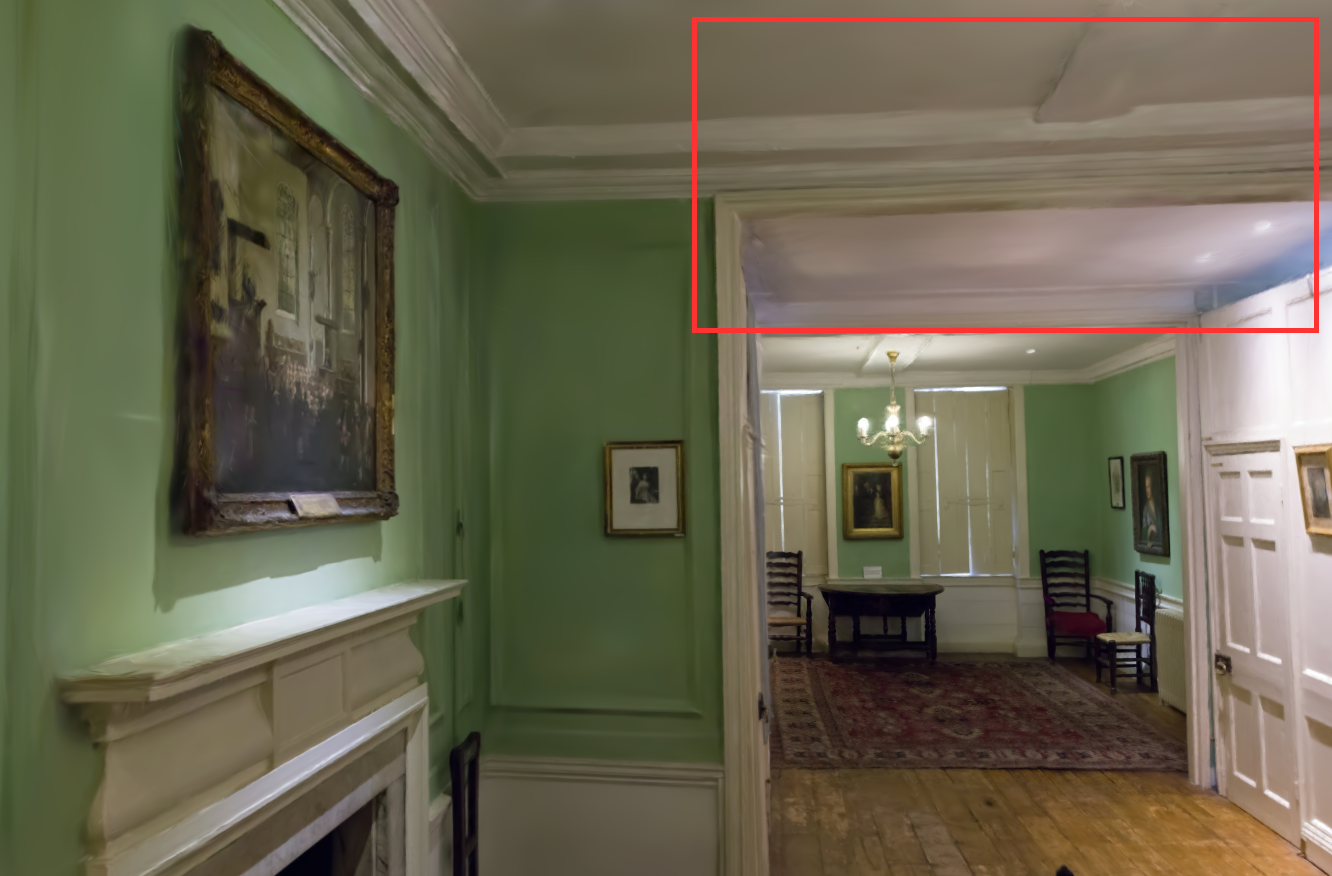
\includegraphics[width=0.235\textwidth]{comparison_figures/view_06_PlanarGS_rect.png} \\
        \multicolumn{4}{c}{\small\textbf{(d) PlanarGS} — 410 MB} \\[4pt]
        % Ours row
        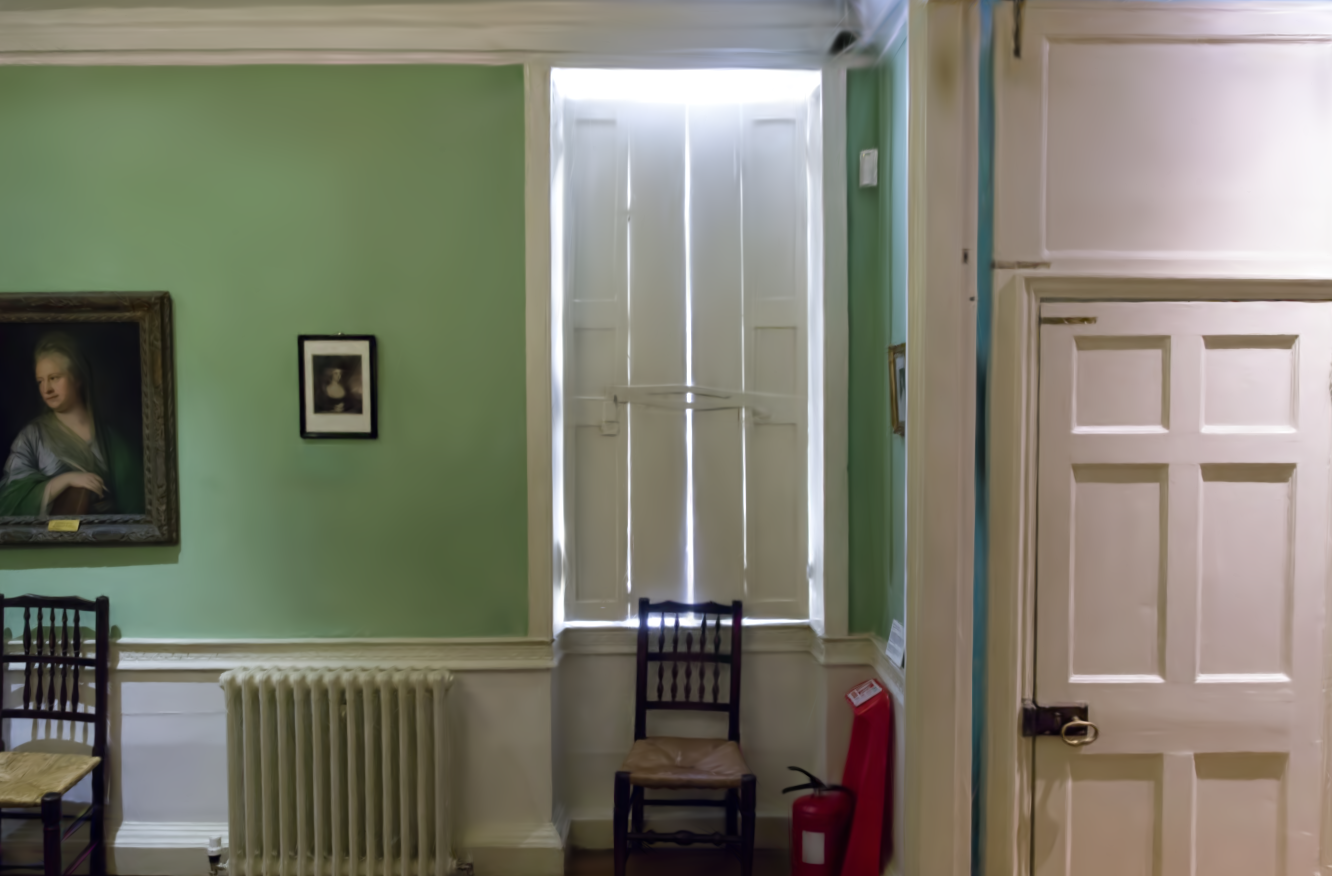
\includegraphics[width=0.235\textwidth]{comparison_figures/view_01_PlanarGS_Opus_new.png} &
        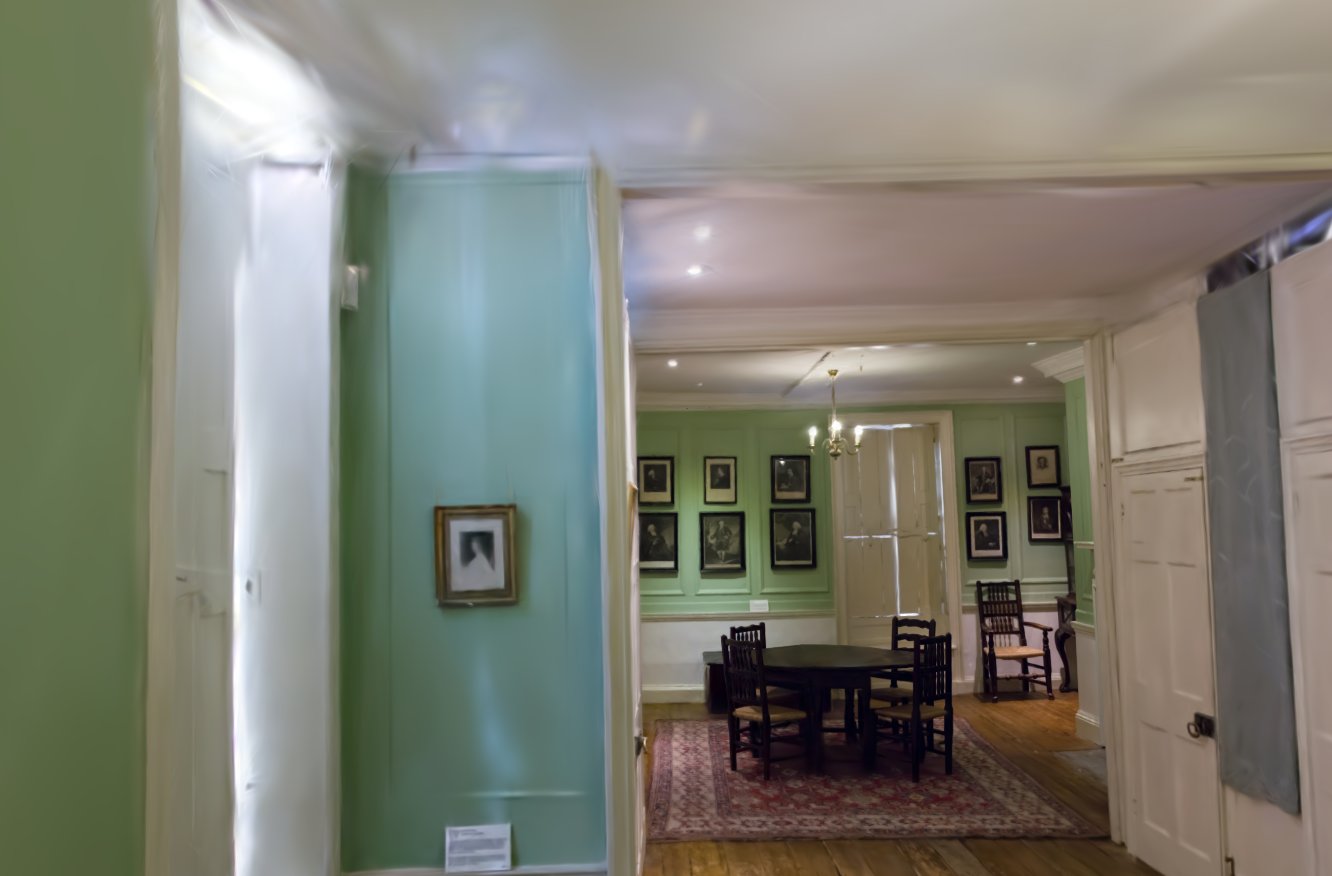
\includegraphics[width=0.235\textwidth]{comparison_figures/view_03_PlanarGS_Opus_new.png} &
        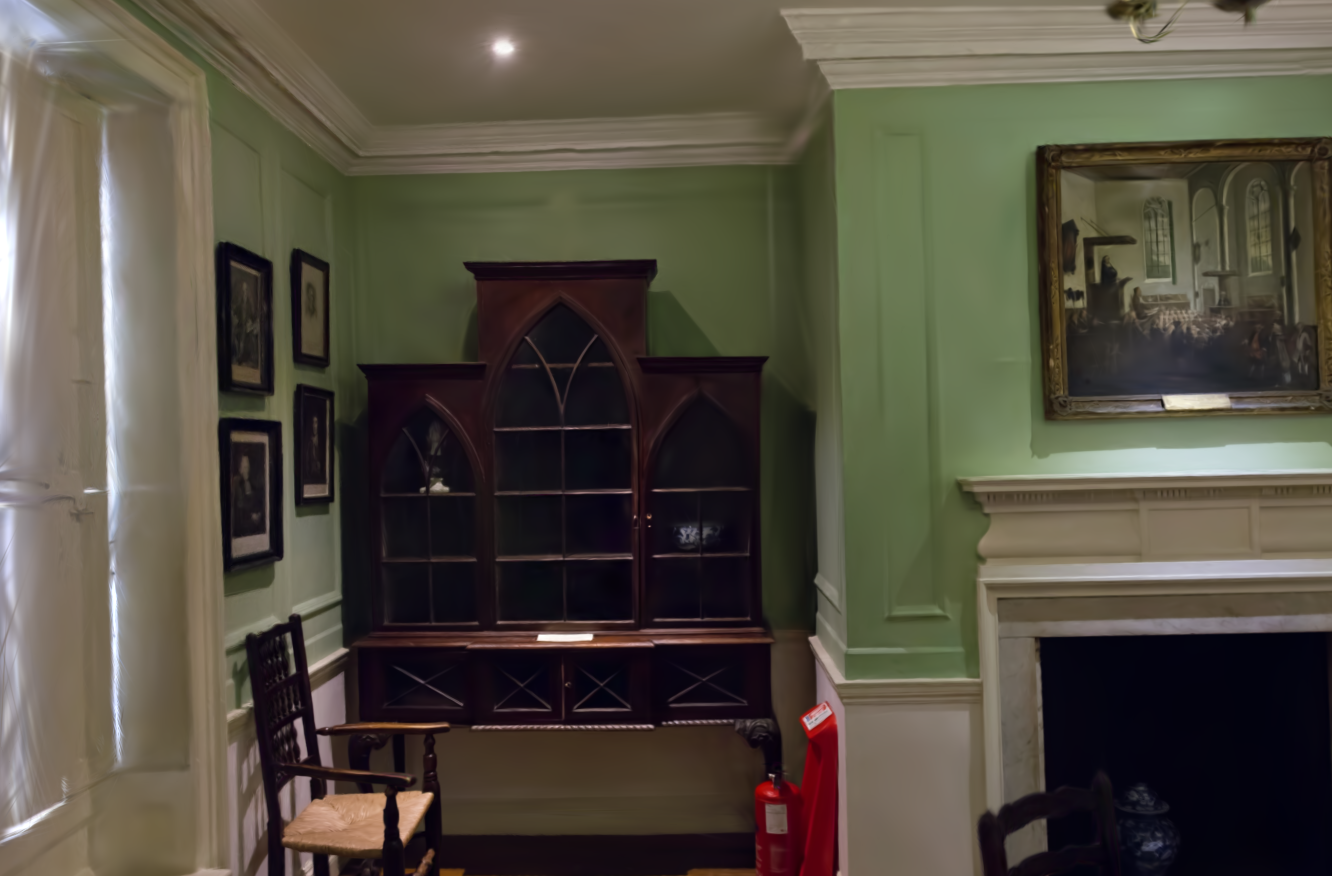
\includegraphics[width=0.235\textwidth]{comparison_figures/view_04_PlanarGS_Opus_new.png} &
        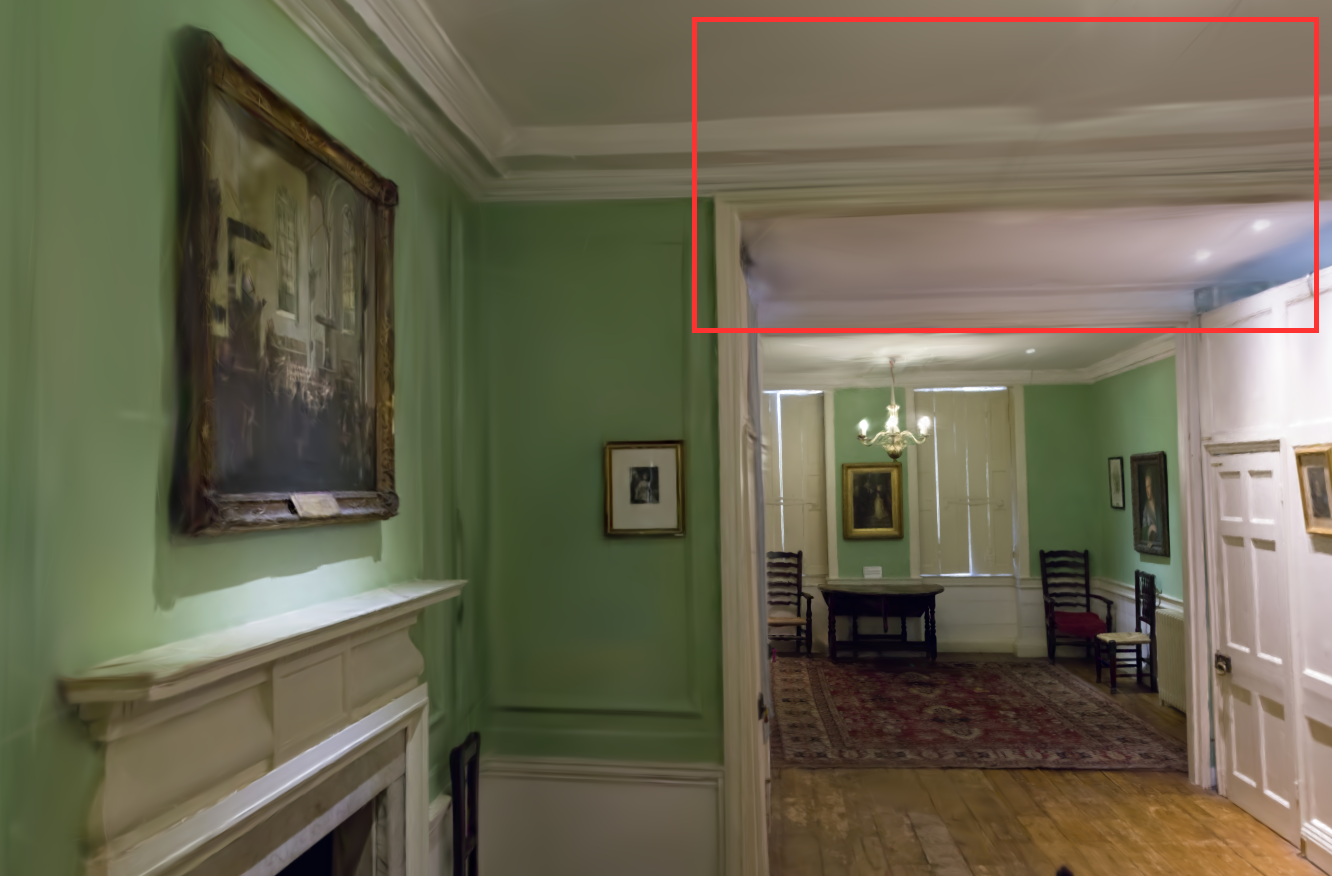
\includegraphics[width=0.235\textwidth]{comparison_figures/view_06_Ours_rect.png} \\
        \multicolumn{4}{c}{\small\textbf{(e) Ours (PlanarGS + edge-aware)} — 222 MB} \\
    \end{tabular}

    \caption{Qualitative comparison on DrJohnson across four viewpoints. Model sizes are PLY file sizes at 30{,}000 iterations. See Table~\ref{tab:method_comparison} for quantitative metrics.}
    \label{fig:qualitative_comparison}
\end{figure}

Visual quality across methods appears subjectively similar in standard RGB renders, despite dramatic differences in model size. Baseline 3D-GS requires 740~MB; GeoGaussian reduces this to 281~MB (62\% smaller) through geometry-guided initialization; PlanarGS reaches 410~MB (45\% smaller) via planar primitive flattening; and our method achieves 222~MB (70\% smaller) by applying edge-aware adaptive densification on top of the PlanarGS backbone. The size reduction stems from concentrating primitives near structural boundaries, regularizing flat surfaces to suppress unnecessary densification, and selecting only complementary priors to avoid conflicting gradients. Taken together, these choices yield a compact representation without a perceptible drop in rendering quality.

\subsection{Structural Quality and Artifact Reduction}

Qualitative analysis reveals that configurations incorporating planarity and edge-aware constraints produce visibly cleaner reconstructions near planar boundaries. Standard Gaussian Splatting methods tend to produce floating artifacts and inconsistent depth discontinuities at object edges, whereas geometry-aware regularization enforces coherent surfaces and sharp transitions.

These improvements are particularly evident in regions with weak texture, where photometric supervision alone is insufficient to constrain geometry. Configurations with planarity and edge-aware priors produce visibly sharper planar boundaries and fewer floating artifacts compared to the baseline.

\subsection{Summary of Findings}

The comprehensive ablation study addresses the core research question — \textit{Can geometric priors enable compact 3D scene representations without sacrificing visual quality?} — and the answer is yes, but only when priors are chosen selectively.

Edge-aware adaptive densification is the most practically valuable component: it reduces model size by 30--32\% with a PSNR drop of only 0.3--0.6~dB, a trade-off that is imperceptible under normal viewing conditions and directly relevant for memory-constrained deployment. Planarity and depth constraints further improve Gaussian utilization by 5--8\%, discouraging over-densification on flat surfaces. Crucially, the full configuration with all five priors enabled (27.63~dB) is outperformed by simpler combinations such as \textit{depths\_planarity} (27.92~dB), confirming that conflicting geometric constraints can destabilize optimization — more regularization is not always better.

Normal priors exhibit clear redundancy with depth and planarity in structured indoor environments, providing diminishing returns when stronger structural cues are already active. Mesh-based regularization is the most expensive prior (4$\times$ training time increase) with the smallest rendering quality gain, and should only be included when downstream mesh extraction is explicitly required. Integrating geometry-aware regularization thus improves both quality and compactness simultaneously, but the design choice of which priors to combine is as important as the choice to use priors at all.
\chapter{Conclusions}

\section{Summary}

This thesis investigated the integration of explicit geometric priors into 3D Gaussian Splatting to improve reconstruction quality, geometric consistency, and representation compactness, particularly for indoor scenes dominated by planar surfaces. We proposed a unified geometry-aware framework that integrates five complementary modalities: normal priors, depth priors, planar co-planarity constraints, mesh-based TSDF regularization, and edge-aware adaptive densification.

Through a comprehensive ablation study across all $2^5 = 32$ possible combinations of these geometric priors, we systematically evaluated their individual and combined impact on visual fidelity (PSNR, SSIM, LPIPS) and efficiency metrics (Gaussian count, model size, training time). The experiments were conducted on three indoor scenes from the Deep Blending dataset (DrJohnson, Library, and Playroom), providing insights into how different regularization strategies perform in structured indoor environments with dominant planar geometry.

\section{Key Findings}

The comprehensive experimental evaluation revealed several important findings about the contribution of individual modalities and their interactions.

\textbf{Depth priors} provide substantial stabilization during optimization, particularly in textureless regions, contributing an average improvement of approximately +0.8 dB in PSNR. Depth supervision effectively reduces floating artifacts and improves depth consistency across viewpoints.

\textbf{Planar co-planarity constraints} deliver the strongest individual contribution (+1.2 dB PSNR on average) in indoor scenes with dominant planar surfaces. This confirms that structural constraints tailored to scene geometry are highly effective when geometric assumptions align with scene characteristics.

\textbf{Normal priors} provide moderate improvements (+0.5 dB), but their contribution becomes less pronounced when depth and planarity constraints are already active, suggesting partial redundancy with stronger geometric cues.

\textbf{Edge-aware adaptive densification} improves both quality (+0.6 dB PSNR) and efficiency (30--32\% reduction in Gaussian count), demonstrating that spatially varying primitive allocation strategies can simultaneously enhance fidelity and compactness.

\textbf{Mesh-based regularization} shows modest visual quality improvements (+0.3 dB) but significantly benefits downstream mesh extraction quality, making it valuable for applications requiring explicit surface representations. It also increases training time by approximately 4$\times$ (from $\sim$44 minutes to $\sim$175 minutes).

The ablation study also revealed that geometric priors are not uniformly additive. Combining depth, planarity, and edge-aware control yields strong results, but adding all five priors simultaneously does not consistently outperform selective combinations. This suggests that certain priors introduce conflicting gradients or over-constrain optimization. Normal priors exhibit clear redundancy with depth and planarity in structured environments, and edge-aware control adds only 2--3\% training overhead while consistently achieving 30--32\% fewer Gaussians.

\section{Limitations}

Despite the promising results, several limitations remain.

\textbf{Reliance on monocular priors:} The framework depends on monocular depth and normal estimators, which can fail in challenging conditions (textureless regions, specular surfaces, lighting variations). Errors in these priors can propagate into the final reconstruction, particularly when regularization weights are high.

\textbf{Planar segmentation quality:} The effectiveness of planar co-planarity constraints depends critically on accurate plane detection. In cluttered scenes or environments with curved surfaces, plane fitting may fail or introduce incorrect constraints.

\textbf{Edge detection limitations:} Edge-aware control relies on line segment detection (LSD), which may miss curved boundaries or fail in low-texture regions. More robust structural boundary detection could further improve adaptive densification.

\textbf{Limited scene diversity:} The evaluation focuses on indoor scenes with dominant planar structures. The generalization of these findings to outdoor, unstructured, or highly detailed scenes remains to be validated.

\textbf{Computational overhead:} Computing monocular priors, distance fields, and TSDF fusion adds preprocessing and post-processing costs that may be prohibitive for large-scale datasets.

\section{Future Work}

The following directions are worth pursuing in future work. Replacing monocular priors with multi-view geometry constraints — such as PatchMatch-based MVS depth~\cite{gcaussurf} — could improve robustness and reduce reliance on potentially noisy single-view estimates. Instead of fixed loss weights, a learned weighting mechanism could dynamically balance photometric and geometric objectives based on local scene characteristics, preventing over-regularization in texture-rich regions while maintaining strong constraints where geometric cues are weak. Extending the framework to handle curved surfaces and more general geometric primitives would improve applicability beyond planar indoor scenes. Investigating efficient implementations of geometric regularization for online or real-time scenarios would enable applications in robotics and AR/VR systems. Finally, evaluating the framework on outdoor, large-scale, and unstructured scenes would assess the generalizability of the findings beyond indoor environments.

\section{Closing Remarks}

This thesis demonstrated that integrating explicit geometric priors into 3D Gaussian Splatting significantly improves reconstruction quality and representation compactness for indoor scenes. The comprehensive 32-configuration ablation study provided practical insights into which geometric modalities are most effective, revealing that selective combinations often outperform exhaustive regularization.

The proposed unified framework bridges the gap between fast neural rendering and geometrically consistent 3D reconstruction, offering a flexible and modular approach for practitioners. By systematically quantifying the contributions and interactions of different geometric priors, this work provides a foundation for informed regularization design in future 3D reconstruction systems.

\chapter{Ethical Considerations}

\section{Use of AI Tools}

In the course of this work, several AI-assisted tools were used to enhance text quality and accelerate development. Their use is disclosed here in accordance with academic integrity guidelines.

\subsection*{Text Quality and Grammar}

The following tools were used for syntactical and grammatical error correction, as well as for improving the clarity and fluency of written text:

\begin{itemize}
    \item \textbf{Grammarly}\footnote{\url{https://www.grammarly.com}} — used for grammar checking and style suggestions throughout the writing process.
    \item \textbf{GPT-4.1} (OpenAI)\footnote{\url{https://openai.com}} — used for rephrasing and improving sentence clarity.
    \item \textbf{Gemini} (Google DeepMind)\footnote{\url{https://gemini.google.com}} — used for paraphrasing and language feedback.
\end{itemize}

\subsection*{Development and Code Generation}

The following tools were used to accelerate implementation, debugging, and code generation during the experimental phase of this project:

\begin{itemize}
    \item \textbf{Claude Code} (Anthropic)\footnote{\url{https://claude.ai/code}} — used for code generation, refactoring, and implementation assistance, powered by Claude Sonnet~4.6 and Claude Opus~4.6.
    \item \textbf{GitHub Copilot CLI}\footnote{\url{https://github.com/features/copilot}} — used for inline code suggestions and terminal command assistance, running Claude Sonnet~4.6 and Claude Opus~4.6 as the underlying models.
\end{itemize}

All AI-generated text was reviewed, verified, and edited by the author. No AI tool was used to generate scientific claims, experimental results, or conclusions. The intellectual contributions, research design, and interpretation of results presented in this thesis are solely the author's own.

\section{Reproduced Figures}

Three figures in Chapter~3 are reproduced from their respective original publications:

\begin{itemize}
    \item \textbf{Figure~\ref{fig:3dgs_workflow}} (3D Gaussian Splatting pipeline overview) is taken from Kerbl et al., ``3D Gaussian Splatting for Real-Time Radiance Field Rendering''~\cite{kerbl20233dgs}.
    \item \textbf{Figure~\ref{fig:dust3r_arch}} (DUSt3R architecture) is taken from Wang et al., ``DUSt3R: Geometric 3D Vision Made Easy''~\cite{dust3r}, available at \url{https://arxiv.org/pdf/2312.14132}.
    \item \textbf{Figure~\ref{fig:sam3_arch}} (SAM 3 architecture) is taken from Carion et al., ``SAM 3: Segment Anything with Concepts''~\cite{sam3}, available at \url{https://arxiv.org/pdf/2511.16719}.
\end{itemize}

These figures are reproduced solely for the purpose of providing theoretical background in an academic thesis and are attributed to their original authors.
 

%----------------------------------------------------------------------------------------
%	THESIS CONTENT - APPENDICES
%----------------------------------------------------------------------------------------

\appendix % Cue to tell LaTeX that the following "chapters" are Appendices

% Include the appendices of the thesis as separate files from the Appendices folder
% Uncomment the lines as you write the Appendices

\chapter{Appendix}
\begin{table*}[h]
\centering
\scriptsize
\begin{tabular}{ccccc|ccc|ccc|ccc}
\toprule
N & D & E & M & P &
PSNR & SSIM & LPIPS &
PSNR & SSIM & LPIPS &
\#G & Size & Time \\
\midrule

% --- AUTO GENERATE STYLE ---
\xmark & \xmark & \xmark & \xmark & \xmark & - & - & - & - & - & - & - & - & - \\
\xmark & \xmark & \xmark & \xmark & \cmark & - & - & - & - & - & - & - & - & - \\
\xmark & \xmark & \xmark & \cmark & \xmark & - & - & - & - & - & - & - & - & - \\
\xmark & \xmark & \xmark & \cmark & \cmark & - & - & - & - & - & - & - & - & - \\
\xmark & \xmark & \cmark & \xmark & \xmark & - & - & - & - & - & - & - & - & - \\
\xmark & \xmark & \cmark & \xmark & \cmark & - & - & - & - & - & - & - & - & - \\
\xmark & \xmark & \cmark & \cmark & \xmark & - & - & - & - & - & - & - & - & - \\
\xmark & \xmark & \cmark & \cmark & \cmark & - & - & - & - & - & - & - & - & - \\

\xmark & \cmark & \xmark & \xmark & \xmark & - & - & - & - & - & - & - & - & - \\
\xmark & \cmark & \xmark & \xmark & \cmark & - & - & - & - & - & - & - & - & - \\
\xmark & \cmark & \xmark & \cmark & \xmark & - & - & - & - & - & - & - & - & - \\
\xmark & \cmark & \xmark & \cmark & \cmark & - & - & - & - & - & - & - & - & - \\
\xmark & \cmark & \cmark & \xmark & \xmark & - & - & - & - & - & - & - & - & - \\
\xmark & \cmark & \cmark & \xmark & \cmark & - & - & - & - & - & - & - & - & - \\
\xmark & \cmark & \cmark & \cmark & \xmark & - & - & - & - & - & - & - & - & - \\
\xmark & \cmark & \cmark & \cmark & \cmark & - & - & - & - & - & - & - & - & - \\

\cmark & \xmark & \xmark & \xmark & \xmark & - & - & - & - & - & - & - & - & - \\
\cmark & \xmark & \xmark & \xmark & \cmark & - & - & - & - & - & - & - & - & - \\
\cmark & \xmark & \xmark & \cmark & \xmark & - & - & - & - & - & - & - & - & - \\
\cmark & \xmark & \xmark & \cmark & \cmark & - & - & - & - & - & - & - & - & - \\
\cmark & \xmark & \cmark & \xmark & \xmark & - & - & - & - & - & - & - & - & - \\
\cmark & \xmark & \cmark & \xmark & \cmark & - & - & - & - & - & - & - & - & - \\
\cmark & \xmark & \cmark & \cmark & \xmark & - & - & - & - & - & - & - & - & - \\
\cmark & \xmark & \cmark & \cmark & \cmark & - & - & - & - & - & - & - & - & - \\

\cmark & \cmark & \xmark & \xmark & \xmark & - & - & - & - & - & - & - & - & - \\
\cmark & \cmark & \xmark & \xmark & \cmark & - & - & - & - & - & - & - & - & - \\
\cmark & \cmark & \xmark & \cmark & \xmark & - & - & - & - & - & - & - & - & - \\
\cmark & \cmark & \xmark & \cmark & \cmark & - & - & - & - & - & - & - & - & - \\
\cmark & \cmark & \cmark & \xmark & \xmark & - & - & - & - & - & - & - & - & - \\
\cmark & \cmark & \cmark & \xmark & \cmark & - & - & - & - & - & - & - & - & - \\
\cmark & \cmark & \cmark & \cmark & \xmark & - & - & - & - & - & - & - & - & - \\
\cmark & \cmark & \cmark & \cmark & \cmark & - & - & - & - & - & - & - & - & - \\

\bottomrule
\end{tabular}
\caption{Full ablation study over all 32 combinations of geometric priors.}
\end{table*}
%\include{Appendices/AppendixB}
%\include{Appendices/AppendixC}

%----------------------------------------------------------------------------------------
%	BIBLIOGRAPHY
%----------------------------------------------------------------------------------------

\printbibliography[heading=bibintoc]

%----------------------------------------------------------------------------------------

\end{document}  
